\documentclass[a4paper,11pt]{book}

\usepackage[UTF8]{ctex}
\usepackage{amsmath,amssymb,amsfonts}
\usepackage{graphicx}
\usepackage[margin=2.5cm,top=3cm,bottom=2.5cm]{geometry}
\usepackage{float}
\usepackage{enumitem}
\usepackage{fancyhdr}
\usepackage{titlesec}
\usepackage{setspace}

% Page style
\pagestyle{fancy}
\fancyhf{}
\fancyhead[LE]{\leftmark}
\fancyhead[RO]{\rightmark}
\fancyfoot[C]{\thepage}
\renewcommand{\headrulewidth}{0.4pt}

% Paragraph spacing
\setlength{\parindent}{0pt}
\setlength{\parskip}{6pt}

\begin{document}

\begin{titlepage}
\centering
\vspace*{3cm}
{\Huge\bfseries 力学（第二版）\par}
\vspace{1cm}
{\LARGE 习题做题本\par}
\vspace{0.5cm}
{\Large 张汉壮 编著\par}
\vfill
{\large \today\par}
\end{titlepage}

\newpage

% Part 1
\textbf{1-1.}一质点沿 $x$ 轴方向做直线运动, $t$ 时刻的坐标为 $x(t) = 5t^{2} - t^{3}$ , 式中 $x$ 以 $\mathrm{m}$ 为单位, $t$ 以 $\mathrm{s}$ 为单位。求: (1) 第 $3 \mathrm{~s}$ 至第 $4 \mathrm{~s}$ 内质点的位移和平均速度; (2) 第 $3 \mathrm{~s}$ 至第 $4 \mathrm{~s}$ 内质点所走过的路程。

\vfill

\textbf{1-2.}沿 $x$ 轴运动的质点, 其速度和时间的关系 $v(t) = t^2 + \pi \cos \frac{\pi}{6} t$ (SI 单位)。在 $t = 0$ 时, 质点的位置 $x_0 = -2 \mathrm{~m}$ 。试求: $t_1 = 3 \mathrm{~s}$ 时, (1) 质点的位置; (2) 质点的加速度。

\vfill
\newpage

\textbf{1-3.}一质点沿 $x$ 轴运动, 其加速度与位置的关系为 $a(x) = 2x + 4x^{2}$ (SI 单位), 已知质点在 $x = 0$ 处的速度为 $2 \mathrm{~m} / \mathrm{s}$ , 试求质点在 $x = 3 \mathrm{~m}$ 处的速度。

\vfill

\textbf{1-4.}一质点沿 $x$ 轴做直线运动, 其速度 $v$ 随时间 $t$ 的变化关系如习题1-4图所示。设 $t = 0$ 时, 质点位于坐标原点。试根据习题1-4图分别尽可能准确地画出,

(1) 表示质点运动的加速度 a 随时间 t 变化关系的 a-t 图;

(2) 表示质点运动的位移 $x$ 随时间 $t$ 变化关系的 $x - t$ 图。

\begin{figure}[H]
  \centering
  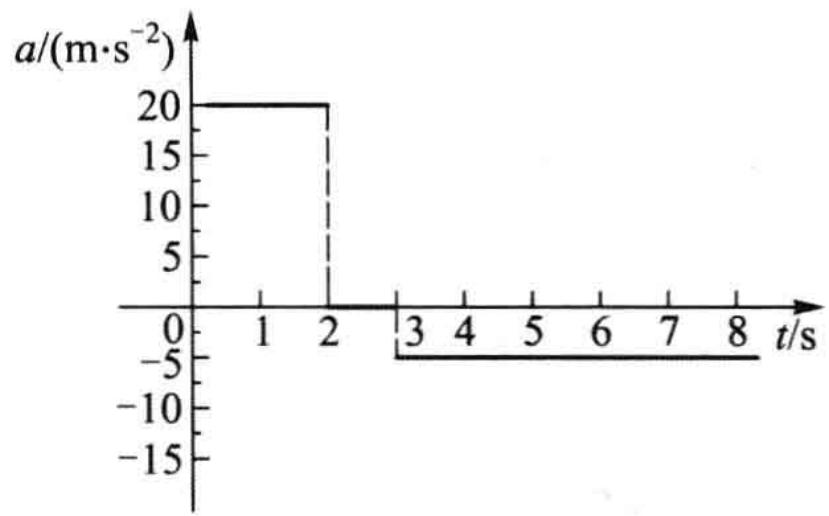
\includegraphics[width=0.4\textwidth]{figures/fig1-4.jpg}
\end{figure}

\vfill
\newpage

\textbf{1-5.}质点的运动学方程为 $r = 3ti + (2t^3 + 1)j$ (SI单位)。求：

(1) 自 $t_{0}=0$ 至 $t_{1}=1$ s 质点的位移；

(2) $t_{0} = 0$ 和 $t_1 = 1 \mathrm{~s}$ 两时刻质点的速度和加速度。

\vfill

\textbf{1-6.}一质点从 $r_0 = -5j$ m 位置开始运动, 其速度与时间的关系为 $v = 2ti + 5j$ , $r$ 以 $\mathrm{m}$ 为单位, $v$ 以 $\mathrm{m/s}$ 为单位。试问:

(1) 经过多少时间质点到达 x 轴?

(2) 此时质点位于 $x$ 轴上哪一点?

\vfill
\newpage

\textbf{1-7.}质点运动学方程为: $r = a \cos \omega t i + a \sin \omega t j + b t k$ , 其中 $a, b, \omega$ 均为正常量, 式中 $r$ 以 $\mathrm{m}$ 为单位, $t$ 以 $\mathrm{s}$ 为单位。

(1) 求质点速度和加速度与时间的关系式;

(2) 问质点做什么运动?

\vfill

\textbf{1-8.}离水面高度为 $h$ 的岸上有人用绳索拉船靠岸。人以恒定速率 $v_{0}$ 拉绳，求当船离岸的距离为 $s$ 时，船的速度和加速度。

\begin{figure}[H]
  \centering
  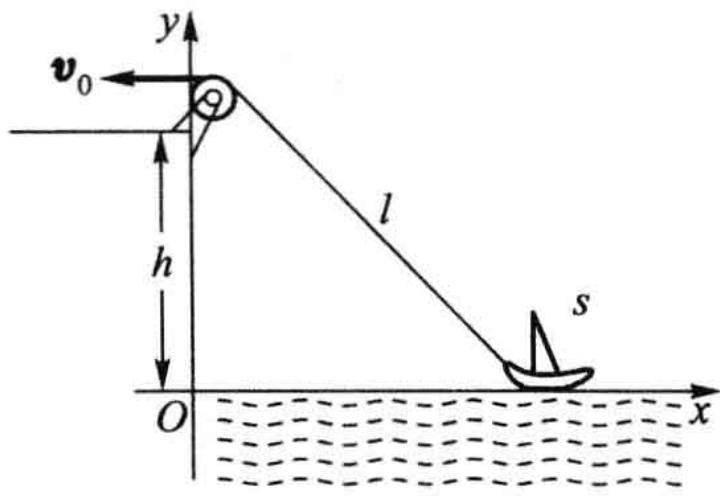
\includegraphics[width=0.3\textwidth]{figures/fig1-8.jpg}
  \end{figure}

\vfill
\newpage

\textbf{1-9.}如习题 1-9 图所示, 在桌面的一边, 一小球做斜抛运动。已知桌面高

$h = 1.0 \mathrm{~m}$ , 宽 $a = 2.0 \mathrm{~m}$ 。若欲使小球能从桌面的另一边切过, 并掉在离该边水平距离 $b = 0.50 \mathrm{~m}$ 处, 求小球的初速度 $v_{0}$ 和抛射角 $\theta$ 。

\begin{figure}[H]
  \centering
  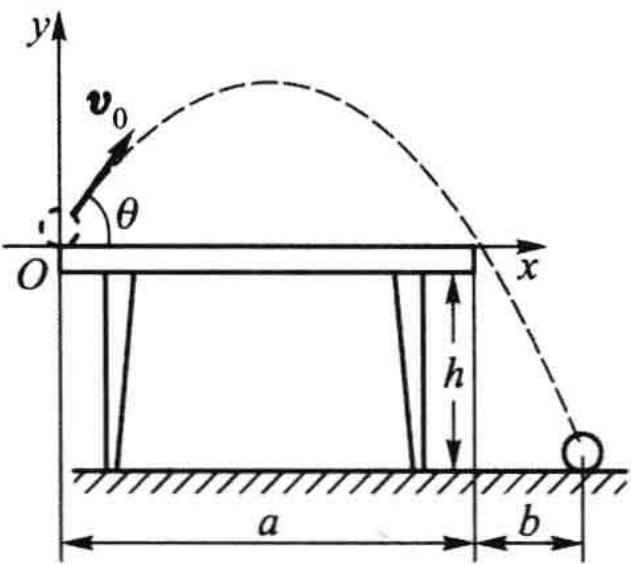
\includegraphics[width=0.3\textwidth]{figures/fig1-9.jpg}
  \end{figure}

\vfill

\textbf{1-10.}杆以匀角速 $\omega_0$ 绕过其固定端 $O$ 且垂直于杆的轴转动。在 $t = 0$ 时, 位于点 $O$ 的小珠从相对于杆静止开始沿杆做加速度为 $a_0$ 的匀加速运动。求小珠在 $t$ 时刻的速度和加速度。

\vfill
\newpage

\textbf{1-11.}有一半径为 $R$ 的定滑轮, 沿轮周绕着一根绳子, 悬在绳子一端的物体

按 $s = \frac{1}{2} bt^2$ 的规律向下运动, 如习题 1-11 图所示。若绳子与轮周间没有相对滑动, 试求轮周上一点 $A$ 在任一时刻 $t$ 的速度、切向加速度、法向加速度和总加速度大小。

\begin{figure}[H]
  \centering
  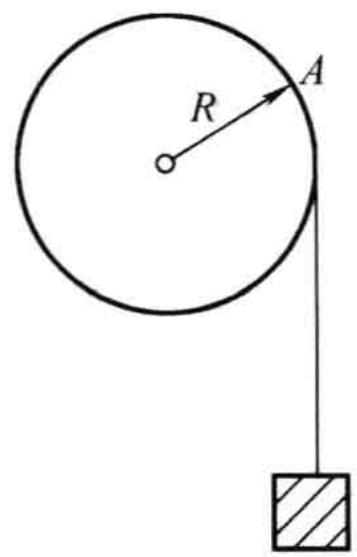
\includegraphics[width=0.2\textwidth]{figures/fig1-11.jpg}
  \end{figure}

\vfill

\textbf{1-12.}当蒸汽船以 $15 \mathrm{~km} / \mathrm{h}$ 的速度向正北方向航行时, 船上的人观察到船上的烟囱里冒出的烟飘向正东方向。过一会儿, 船以 $24 \mathrm{~km} / \mathrm{h}$ 的速度向正东方向航行, 船上的人则观察到烟飘向正西北方向。若在这两次航行期间风速不变, 求风速及方向。

\begin{figure}[H]
  \centering
  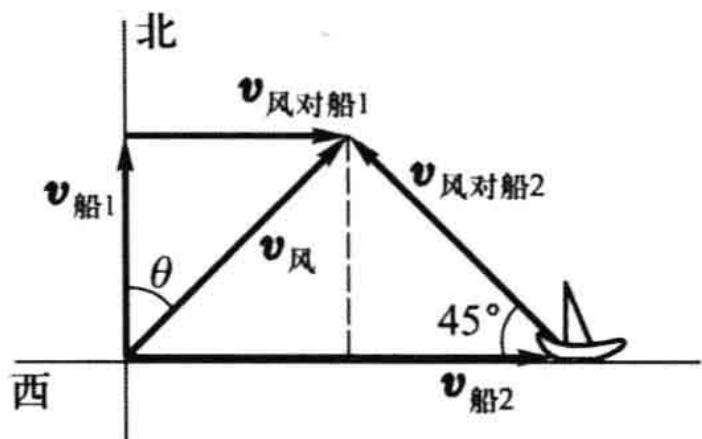
\includegraphics[width=0.3\textwidth]{figures/fig1-12.jpg}
  \end{figure}

\vfill
\newpage


\textbf{1-13.}一个自由落体在它运动的最后 $1 \mathrm{~s}$ 内所通过的路程等于全程的 $\frac{1}{3}$ 。求: (1) 物体下落的高度; (2) 通过全程所需的时间。

\vfill

\textbf{1-14.}一小球做竖直上抛运动,测得小球两次经过 $A$ 点和两次经过 $B$ 点的时间间隔分别为 $\Delta t_{A} 、 \Delta t_{B}$ ,如习题 1-14 图所示。求 $A 、 B$ 两点间的高度差 $h$ 。

\begin{figure}[H]
  \centering
  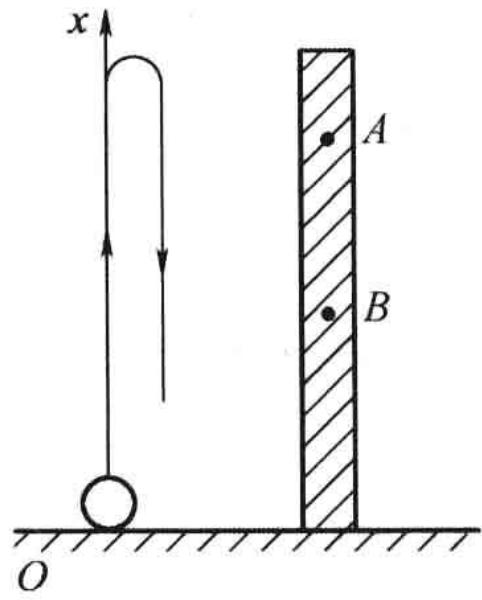
\includegraphics[width=0.25\textwidth]{figures/fig1-14.jpg}
  \end{figure}

\vfill
\newpage

\textbf{1-15.}汽车沿平直公路匀加速行驶,它通过某一段距离 $s$ 所需的时间为 $t_1$ , 而通过下一段相同距离 $s$ 所需的时间为 $t_2$ 。求汽车的加速度。

\vfill

\textbf{1-16.}火车从 A 城由静止开始沿平直轨道驶向 B 城, A、B 两城相距为 $s$ 。火车先以加速度 $a_{1}$ 做匀加速运动, 当速度达到 $v$ 后再匀速行驶一段时间, 然后刹车, 并以加速度大小为 $a_{2}$ 做匀减速行驶, 使之正好停在 B 城。求火车行驶的时间 $t$ 。

\vfill
\newpage

\textbf{1-17.}如习题 1-17 图所示, 物体从具有共同底边, 但倾角不同的若干光滑斜面顶端由静止开始自由滑下。问当倾角为何值时, 才能使物体滑至底端所需的时间最短?

\begin{figure}[H]
  \centering
  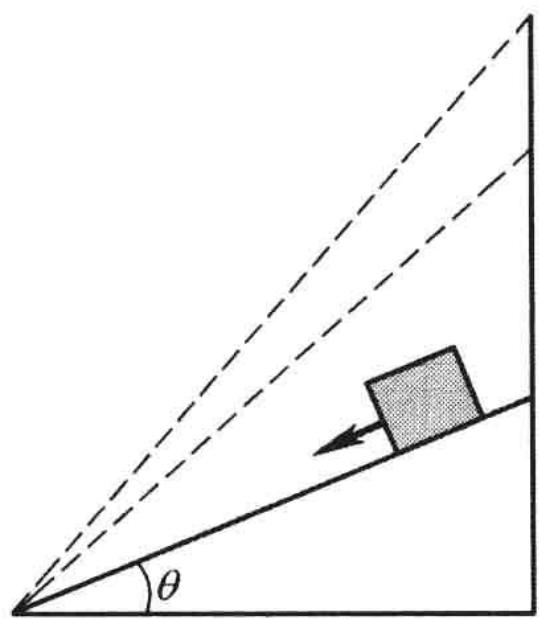
\includegraphics[width=0.25\textwidth]{figures/fig1-17.jpg}
  \end{figure}

\vfill

\textbf{1-18.}石块从楼顶以 $v_{0} = 10 \mathrm{~m} / \mathrm{s}$ 的速度被水平抛出, 落地时速度方向与水平方向之间成 $60^{\circ}$ 角, 求楼房的高度。

\vfill
\newpage

\textbf{1-19.}一物体被水平抛出,经过 $2.5 \mathrm{~s}$ 后,它的速度与加速度之间的夹角为 $45^{\circ}$ ,问又经过多少秒,它的速度与加速度之间的夹角变为 $30^{\circ}$ 。

\vfill

\textbf{1-20.}一小球从离地面高为 $h$ 的 $A$ 点处自由下落。当它下落了 $h_0$ 时, 与一斜面发生碰撞, 并以原速水平弹出, 如习题 1-20 图所示。问 $h_0$ 为多大时, 小球弹得最远?

\begin{figure}[H]
  \centering
  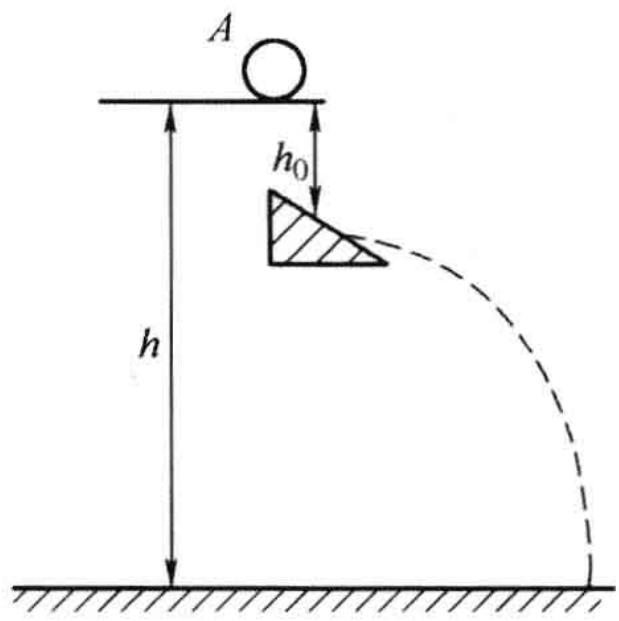
\includegraphics[width=0.3\textwidth]{figures/fig1-20.jpg}
  \end{figure}

\vfill
\newpage

\textbf{1-21.}斜向上抛出一物体,经过一段时间物体仍然向斜上方运动,此时速度方向与水平面成 $45^{\circ}$ 角,又过了相同的时间,物体已向斜下方运动,但速度方向与水平面仍成 $45^{\circ}$ 角。求物体的抛射角。

\vfill

\textbf{1-22.}在与水平面成 $\theta$ 角的山坡上, 一石块以 $v_{0}$ 的初速度做斜抛运动, 如习题 1-22 图所示。

(1) 若抛射角为 $\phi$ (抛出速度与水平面夹角), 求石块沿山坡方向的射程 $s$ ;

(2) 问抛射角 $\phi$ 为多大时, s 最大?

\begin{figure}[H]
  \centering
  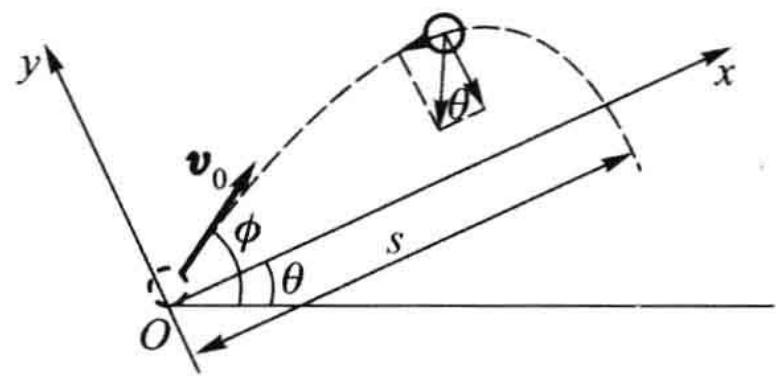
\includegraphics[width=0.4\textwidth]{figures/fig1-22.jpg}
  \end{figure}

\vfill
\newpage

\textbf{1-23.}从原点在竖直平面内以相同的初速度 $v_{0}$ 向各个方向投出许多质点。试证明：

(1) 任何时刻这些质点都处在同一圆周上;

(2) 它们的最高点位于同一椭圆上。

\vfill

\textbf{1-24.}汽车沿一圆周以 $v_{0} = 7.0 \mathrm{~m} / \mathrm{s}$ 的初速度匀减速行驶。经过 $t_{1} = 5 \mathrm{~s}$ 后，汽车的加速度与速度之间的夹角 $\theta_{1} = 135^{\circ}$ 。又经过 $t_{2} = 3 \mathrm{~s}$ 后，其加速度与速度之间的夹角 $\theta_{2} = 150^{\circ}$ 。求：

(1) 圆的半径 R;

(2) 切向加速度 $a_{\tau}$ ;

(3) 这两时刻的法向加速度 $a_{n1}$ 和 $a_{n2}$ 。

\begin{figure}[H]
  \centering
  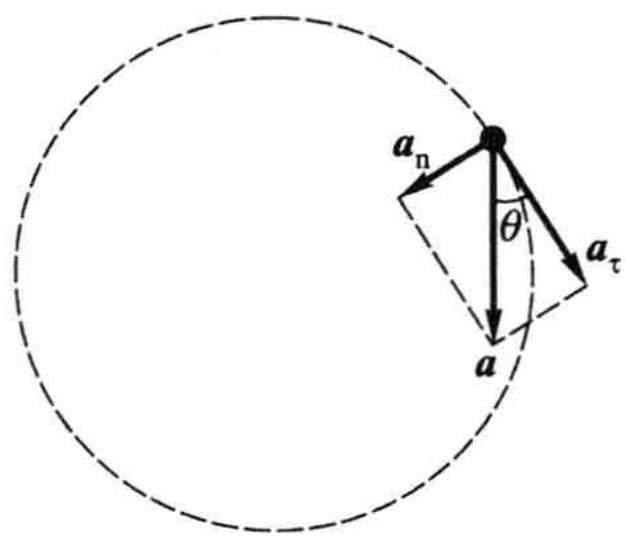
\includegraphics[width=0.3\textwidth]{figures/fig1-24.jpg}
  \end{figure}

\vfill
\newpage

\textbf{1-25.}一摩托车沿着半径 $R = 64 \mathrm{~m}$ 的圆周以 $v_{0} = 1 \mathrm{~m} / \mathrm{s}$ 的初速度行驶, 其切向加速度与时间的数值关系为 $a_{\tau} = \frac{1}{2 \sqrt{t + 1}}$ (SI 单位), 问 $t$ 为多少时, 总加速度最小?

\vfill

\textbf{1-26.}A 船以 $30 \mathrm{~km} / \mathrm{h}$ 的速度向东航行, B 船以 $45 \mathrm{~km} / \mathrm{h}$ 的速度向正北航行。求 A 船上的人观察到的 B 船的航速和航向。

\begin{figure}[H]
  \centering
  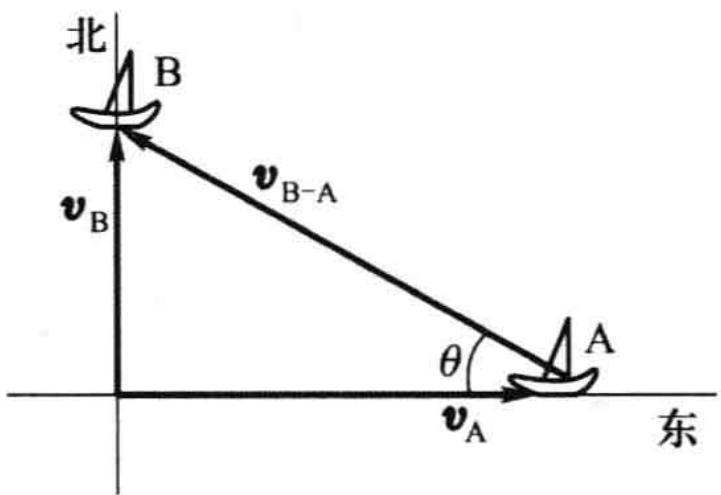
\includegraphics[width=0.4\textwidth]{figures/fig1-26.jpg}
  \end{figure}

\vfill
\newpage

\textbf{1-27.}一溜冰者在冰面上以 $v_{0} = 7 \mathrm{~m} / \mathrm{s}$ 的速度沿半径 $R = 35 \mathrm{~m}$ 的圆周溜冰。某时刻他平抛出一小球, 为使小球能击中冰面的圆心处, 他应以多大的相对于他的速度抛球? 并求出该速度的方向 (用与他溜冰速度之间的夹角 $\theta$ 表示)。已知人抛球时手的高度 $h = 1.5 \mathrm{~m}$ 。

\begin{figure}[H]
  \centering
  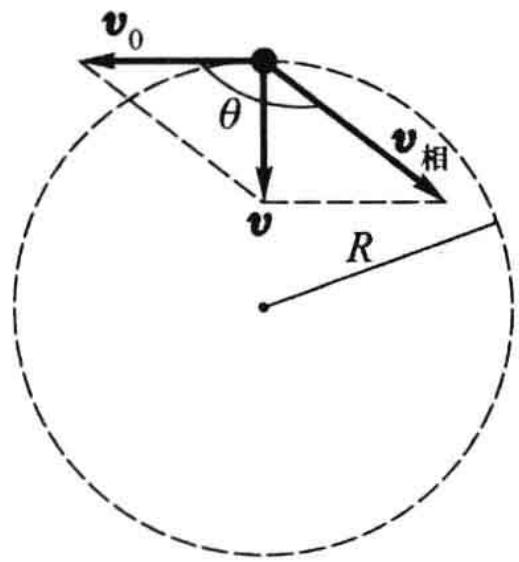
\includegraphics[width=0.25\textwidth]{figures/fig1-27.jpg}
  \end{figure}

\vfill

\textbf{1-28.}在宽为 $l$ 的河的两岸停着两艘小船, 它们的连线与河岸线成 $\alpha$ 角。已知两艘小船在静水中最大的划行速度分别为 $u_{1}$ 和 $u_{2}$ , 河水流速为 $v$ 。若它们同时出发, 则各应向什么方向划行才能在最短的时间内相遇? 并求出此时间。

\begin{figure}[H]
  \centering
  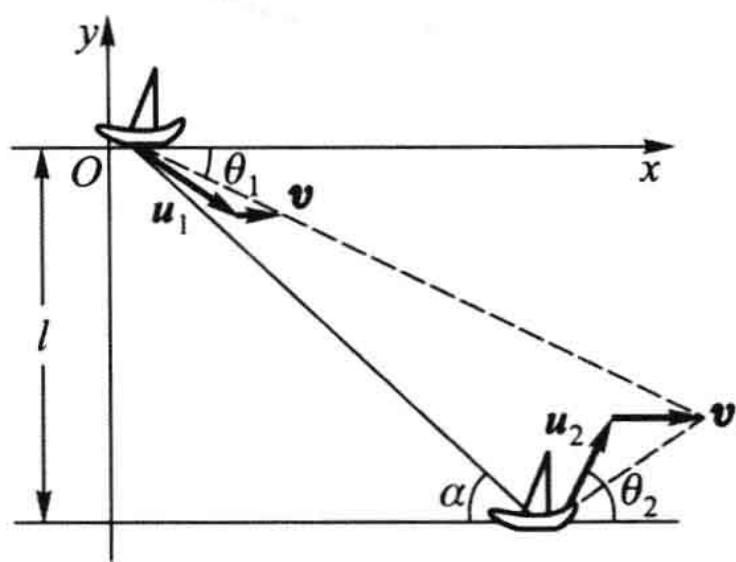
\includegraphics[width=0.3\textwidth]{figures/fig1-28.jpg}
  \end{figure}

\vfill
\newpage

\textbf{1-29.}一架飞机在无风时以匀速 $v$ 相对地面飞行, 能飞出的最远距离为 $R$ (包括飞出和飞回)。现在风速为 $u$ , 方向为北偏东、角度为 $\alpha$ 的风中飞行, 而飞行的实际航向为北偏东、角度为 $\beta$ 。求证: 在这种情况下, 飞机能飞出的最远距

$$
\frac {R \left(v ^ {2} - u ^ {2}\right)}{v \sqrt {v ^ {2} - u ^ {2} \sin^ {2} (\beta - \alpha)}}
$$

\begin{figure}[H]
  \centering
  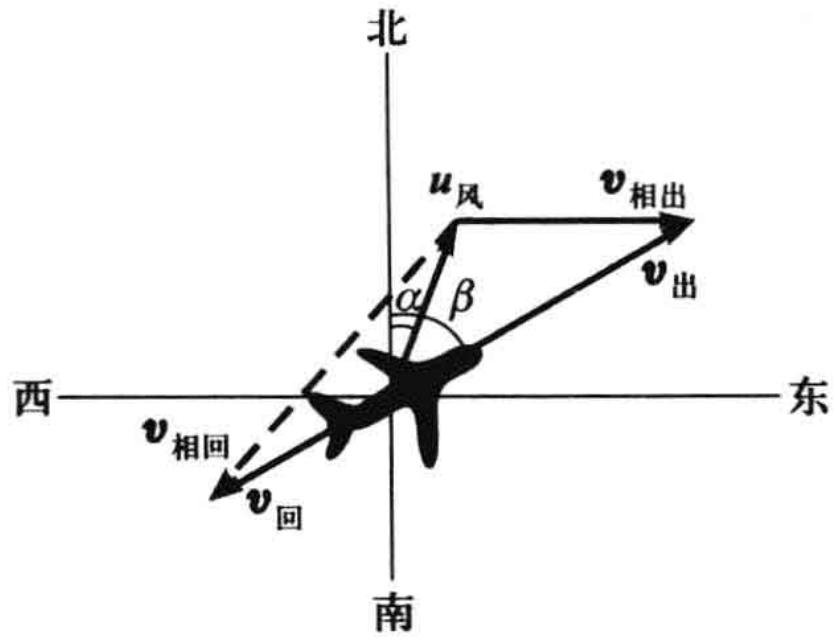
\includegraphics[width=0.4\textwidth]{figures/fig1-29.jpg}
  \end{figure}

\vfill
\newpage

\textbf{2-1.}在习题 2-1 图中, 人的质量 $m_{1} = 60 \mathrm{~kg}$ , 底板的质量 $m_{2} = 40 \mathrm{~kg}$ 。人若

想站在底板上静止不动,则必须以多大的力拉住绳子?

\begin{figure}[H]
  \centering
  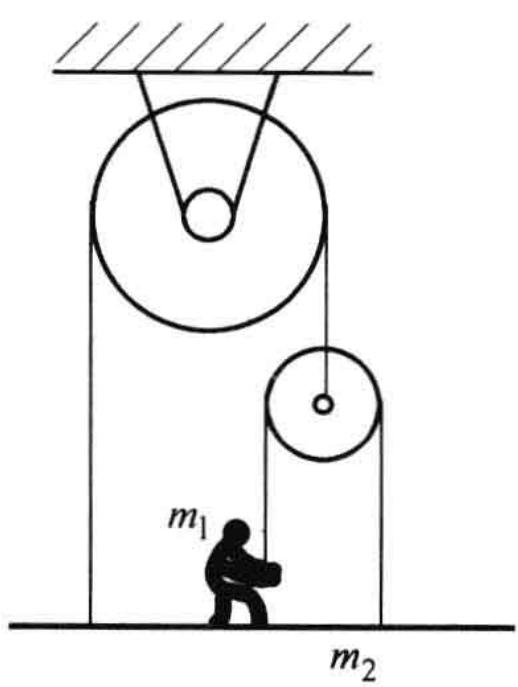
\includegraphics[width=0.2\textwidth]{figures/fig2-1.jpg}
  \end{figure}

\vfill

\textbf{2-2.}一根质量为 $m_{0}$ 的均质绳子, 两端固定在同一高度的两个钉子上, 在其中点挂一质量为 $m$ 的物体。设 $\alpha, \beta$ 分别为在绳子中点和端点处绳子的切线方向与竖直方向的夹角, 如习题 2- 2 图所示。求 $\frac{\tan \alpha}{\tan \beta}$ 与 $m_{0}, m$ 的关系。

\begin{figure}[H]
  \centering
  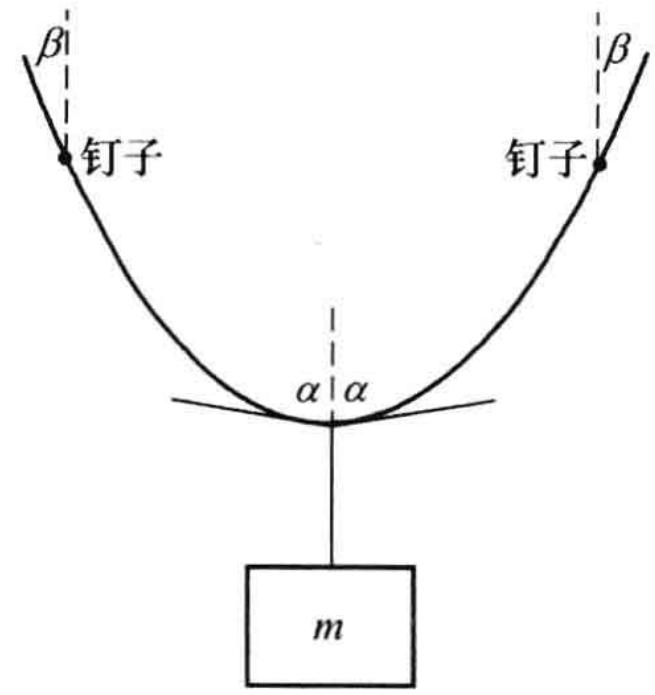
\includegraphics[width=0.25\textwidth]{figures/fig2-2.jpg}
  \end{figure}

\vfill
\newpage

\textbf{2-3.}如习题 2-3 图(a)所示,一长为 $l$ 、质量为 $m$ 的均匀链条套在一表面光滑、顶角为 $\alpha$ 的圆锥上,当链条在圆锥面上静止时,求链中的张力。

\begin{figure}[H]
  \centering
  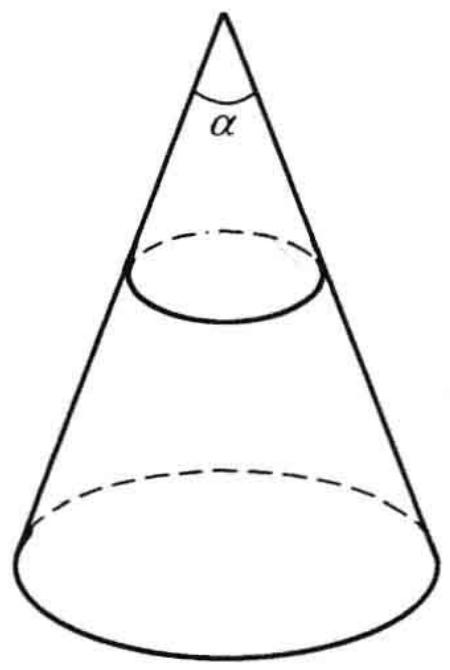
\includegraphics[width=0.2\textwidth]{figures/fig2-3_a.jpg}
  \end{figure}

\vfill

\textbf{2-4.}一条绳索的一端系到停泊在河中的小船上,另一端由站在岸上的人拿着。人正欲收绳把船拉往岸边时,突然刮起了大风,风把船吹向河心。为了不让风把船吹走,人把绳索在岸边的固定圆柱上缠绕若干圈后再拉住绳索。若由于大风使船与圆柱间的绳索中的张力变为 $50000 \mathrm{~N}$ , 而人拉绳的最大力为 $500 \mathrm{~N}$ 。已知绳索与圆柱之间的摩擦因数为 0.32 ,问绳索至少在圆柱上绕几圈,船才不会被吹走?

\begin{figure}[H]
  \centering
  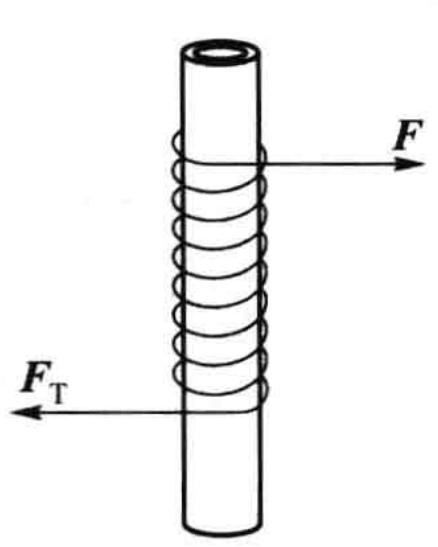
\includegraphics[width=0.2\textwidth]{figures/fig2-4_a.jpg}
  \end{figure}

\vfill
\newpage

\textbf{2-5.}在习题 2-5 图中, 物体 A 和 B 的质量分别为 $m_{\mathrm{A}}$ 和 $m_{\mathrm{B}}$ , 用跨过定滑轮

的细线相连,静止地叠放在倾角为 $\theta$ 的斜面上,各接触面的静摩擦因数为 $\mu$ ,现有一平行于斜面的力 F 作用在物体 A 上,问 F 至少为多大才能使两物体运动?

\begin{figure}[H]
  \centering
  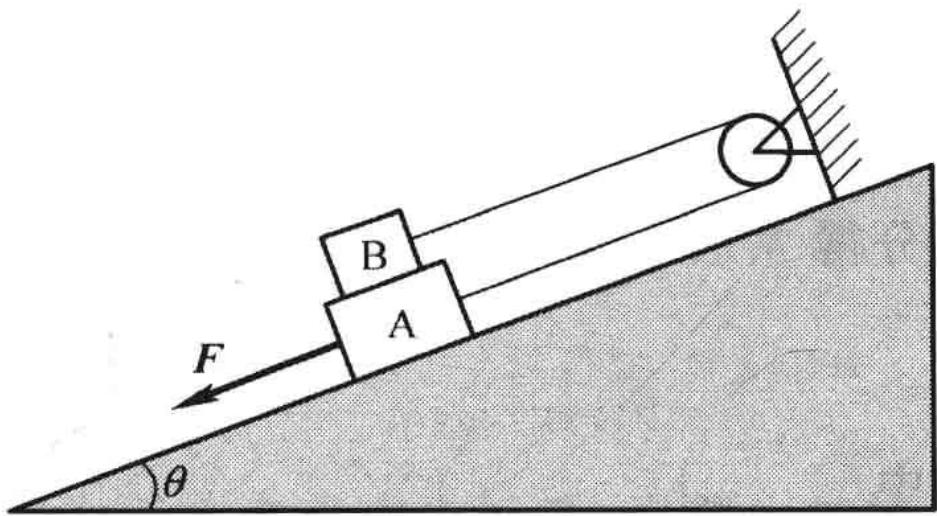
\includegraphics[width=0.3\textwidth]{figures/fig2-5.jpg}
  \end{figure}

\vfill

\textbf{2-6.}质量为 $m_{1}$ 的气球以加速度 $a$ 匀加速上升, 突然一只质量为 $m_{2}$ 的小鸟飞到气球上, 并停留在气球上。若气球仍能向上加速, 求气球的加速度减少了多少?

\vfill
\newpage

\textbf{2-7.}一质量为 $m$ 的汽艇在湖水中以速率 $v_{0}$ 直线运动, 当关闭发动机后, 受水的阻力为 $F_{\mathrm{f}} = -k v$ , 求速度、位移随时间的变化关系。

\vfill

\textbf{2-8.}质量分别为 $m_{1}$ 和 $m_{2}(m_{2} > m_{1})$ 的两个人, 分别拉住跨在定滑轮 (忽略质量) 上的轻绳两边往上爬。开始时两人至定滑轮的距离都是 $h$ 。试证明: 质量为 $m_{1}$ 的人经过时间 $t$ 爬到滑轮处时, 质量为 $m_{2}$ 的人与滑轮的距离为 $\frac{m_{2} - m_{1}}{m_{2}}\left(h + \frac{1}{2}gt^{2}\right)$ 。

\begin{figure}[H]
  \centering
  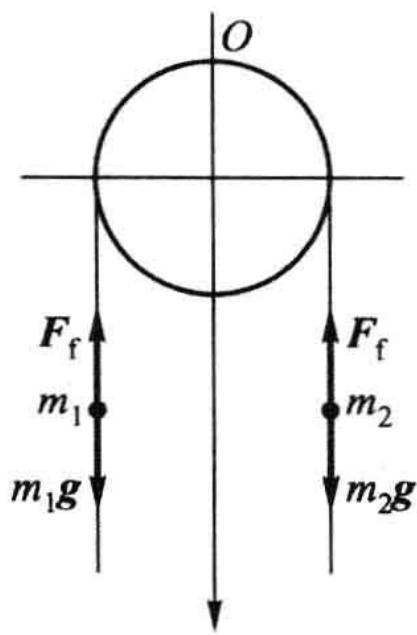
\includegraphics[width=0.2\textwidth]{figures/fig2-8.jpg}
  \end{figure}

\vfill
\newpage

\textbf{2-9.}一物体以 $v_{0}$ 的初速度做竖直上抛运动, 若受到的阻力 $F_{\mathrm{f}}$ 与其速度的二次方 $v^{2}$ 成正比, 大小可表示为 $F_{\mathrm{f}} = m g k^{2} v^{2}$ , 其中 $m$ 为物体的质量, $k$ 为常量。试证明此物体回到上抛点时的速度为 $v_{1} = \sqrt{\frac{v_{0}^{2}}{1 + (k v_{0})^{2}}}$ 。

\vfill

\textbf{2-10.}一半顶角为 $\alpha$ 的倒立圆锥面的内表面光滑, 内表面上一质点绕对称轴做半径为 $r$ 的匀速圆周运动。求质点的速率。

\vfill
\newpage

\textbf{2-11.}如习题 2-11 图所示, 两个物体的质量分别为 $m_{1} = 15 \mathrm{~kg}, m_{2} = 20 \mathrm{~kg}$ , 作用在物体 $m_{1}$ 上的水平力 $F = 280 \mathrm{~N}$ 。设所有接触面都光滑。试求:

(1) $m_{1}$ 的加速度的大小和方向；

(2) $m_{2}$ 的加速度的大小和方向；

(3) 两物体间的相互作用力。

\begin{figure}[H]
  \centering
  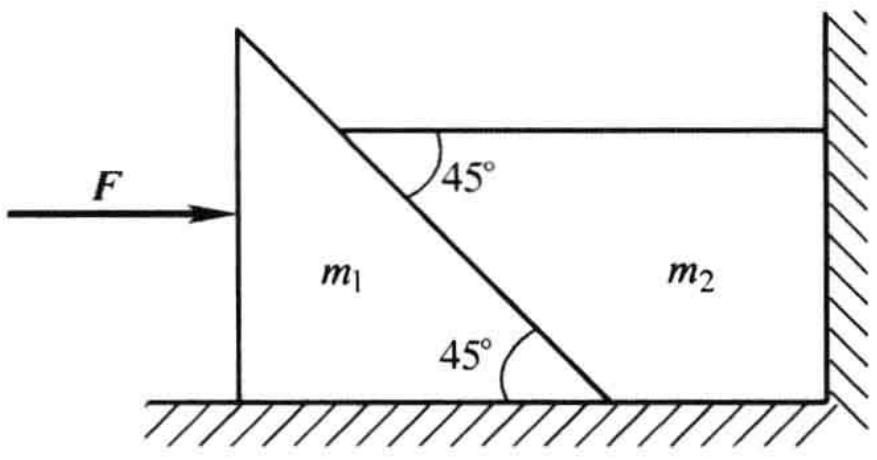
\includegraphics[width=0.3\textwidth]{figures/fig2-11.jpg}
  \end{figure}

\vfill

\textbf{2-12.}从地面以相对地面成 $\theta_0$ 仰角、 $v_0$ 的速度发射一炮弹, 炮弹在运动过程中始终受到与速度成正比的阻力 $F_{\mathrm{f}} = kv (k$ 为常量) 作用, 求炮弹的运动轨迹方程。

\vfill
\newpage



\textbf{2-13.}如习题 2-13 图所示的系统, 系统中人的质量 $m_{1} = 60 \mathrm{~kg}$ , 人所站着的底板质量 $m_{2} = 20 \mathrm{~kg}$ , 绳子和滑轮质量均可忽略不计。人要用多大的力拉住绳子, 才能保持自己和底板静止不动?

\begin{figure}[H]
  \centering
  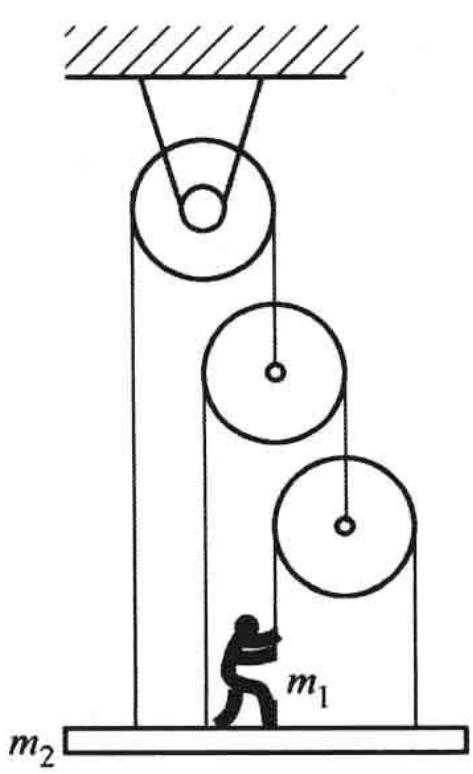
\includegraphics[width=0.2\textwidth]{figures/fig2-13_2.jpg}
  \end{figure}

\vfill

\textbf{2-14.}质量为 $m_{1}$ 和 $m_{2}$ 的两物体, 在水平力 $F$ 的作用下紧靠在墙上, 如习题 2-14 图所示。为使两物块均不掉下, 试问在以下两种情况下, $F$ 至少应为多大?

(1) 各接触面间的静摩擦因数均为 $\mu$ 时；

(2) $m_{1}, m_{2}$ 之间的静摩擦因数为 $\mu_{1}, m_{2}$ 与墙面间的静摩擦因数为 $\mu_{2}$ 时。

\begin{figure}[H]
  \centering
  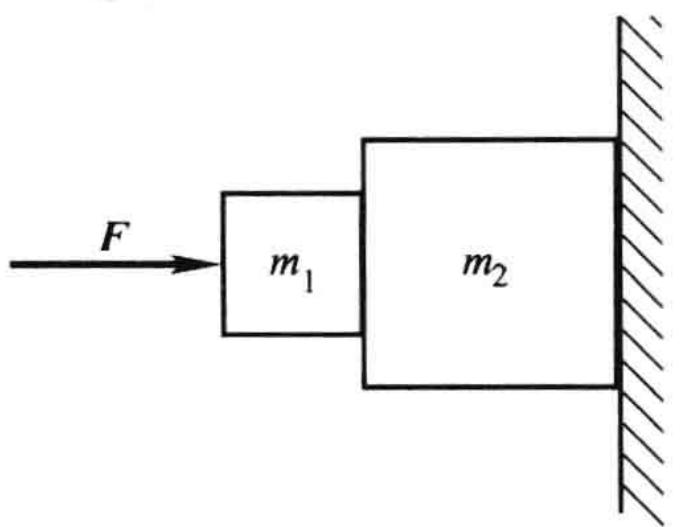
\includegraphics[width=0.3\textwidth]{figures/fig2-14.jpg}
  \end{figure}

\vfill
\newpage

\textbf{2-15.}一个三棱柱固定在桌面上, 形成两个倾角分别为 $\alpha$ 和 $\beta$ 的斜面, 一细绳跨过顶角处的滑轮与质量分别为 $m_{1}$ 和 $m_{2}$ 的两物体相连, 如习题 2-15 图所示。已知物体与斜面间的静摩擦因数均为 $\mu$ , 求两物体在斜面上保持静止的条件。

\begin{figure}[H]
  \centering
  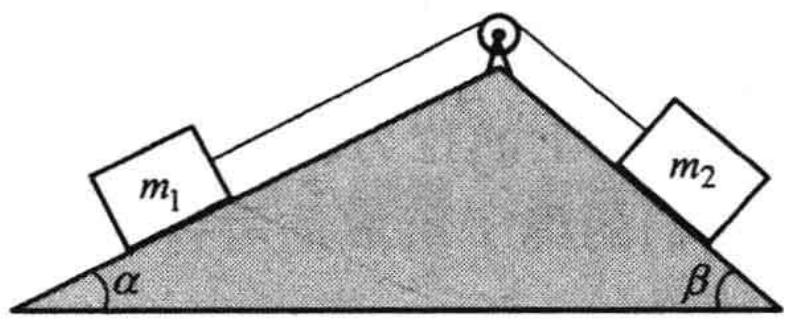
\includegraphics[width=0.3\textwidth]{figures/fig2-15.jpg}
  \end{figure}

\vfill

\textbf{2-16.}三块质量均为 $m$ 的相同物块叠放在水平面上, 如习题 2-16 图所示。已知各接触面的摩擦因数均为$\mu$。

(1) 现有一水平力 F 作用在最底下的物块上, 使之从上面两物块下抽出, 则 F 至少为多大?

(2) 若水平力 $F$ 作用在中间的物块上,使它从上、下两物块中抽出, 则 $F$ 至少为多大?

\begin{figure}[H]
  \centering
  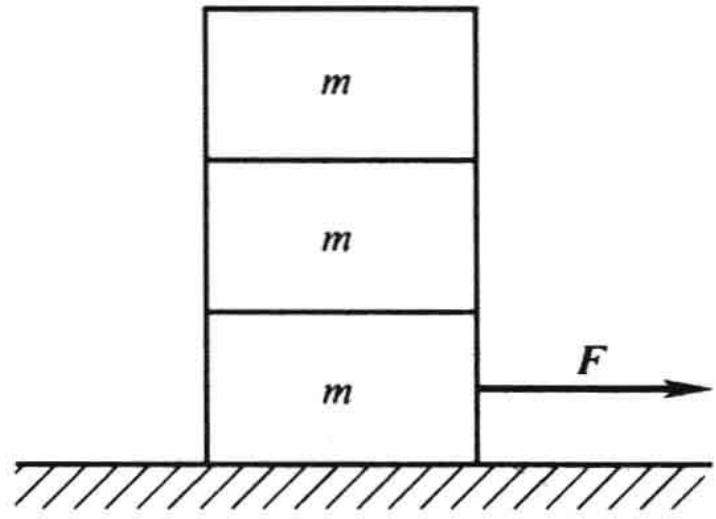
\includegraphics[width=0.3\textwidth]{figures/fig2-16.jpg}
  \end{figure}

\vfill
\newpage

\textbf{2-17.}如习题 2-17 图所示, 质量分别为 $m_{1}$ 和 $m_{2}$ 的两物体用一细绳相连, 细绳跨过装在另一质量为 $m_{0}$ 的大物体上的定滑轮, 使 $m_{1}$ 和 $m_{2}$ 分别与 $m_{0}$ 上的水平面和倾角为 $\theta$ 的斜面接触, 而整个系统放在水平地面上。设 $m_{1}, m_{2}$ 与 $m_{0}$ 间的接触面都光滑。试问, 若要 $m_{0}$ 保持静止, 则 $m_{0}$ 与水平地面之间的摩擦因数至少为多大?

\begin{figure}[H]
  \centering
  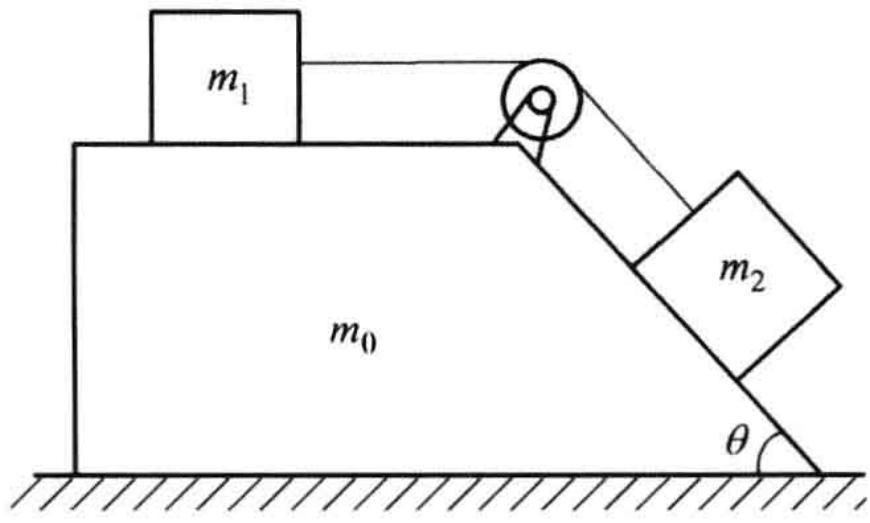
\includegraphics[width=0.3\textwidth]{figures/fig2-17.jpg}
  \end{figure}

\vfill

\textbf{2-18.}一条质量为 $m$ 的均匀绳索悬结于两座高度相等的山顶之间, 绳索在悬结处与竖直方向的夹角均为 $\theta$ , 如习题 2-18 图所示。试求:

(1) 两山顶各自受到的绳索的作用力的大小;

(2) 绳索中点处的张力。

\begin{figure}[H]
  \centering
  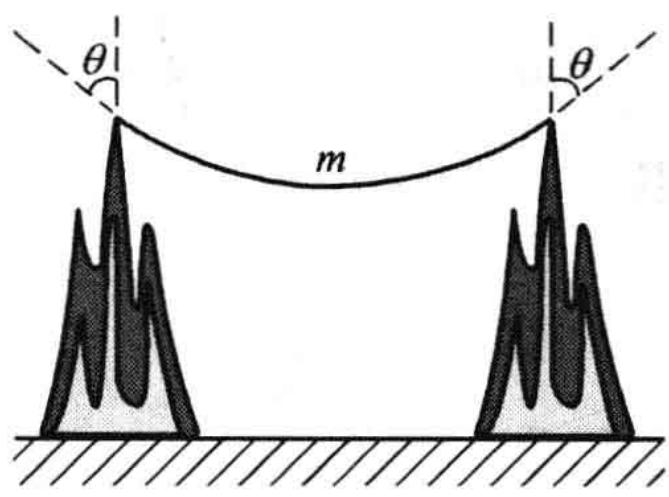
\includegraphics[width=0.3\textwidth]{figures/fig2-18_x.jpg}
  \end{figure}

\vfill
\newpage

\textbf{2-19.}一个质量为 $m$ 的物体通过一根质量可以不计的绳子绕水平棒 $1 \frac{1}{4}$ 周后于另一端加一水平力 $F$ , 如习题 2-19 图 (a) 所示。若绳子和棒之间的摩擦因数为 $\mu$ , 要使物体保持静止状态, 应施加多大的水平拉力?

\begin{figure}[H]
  \centering
  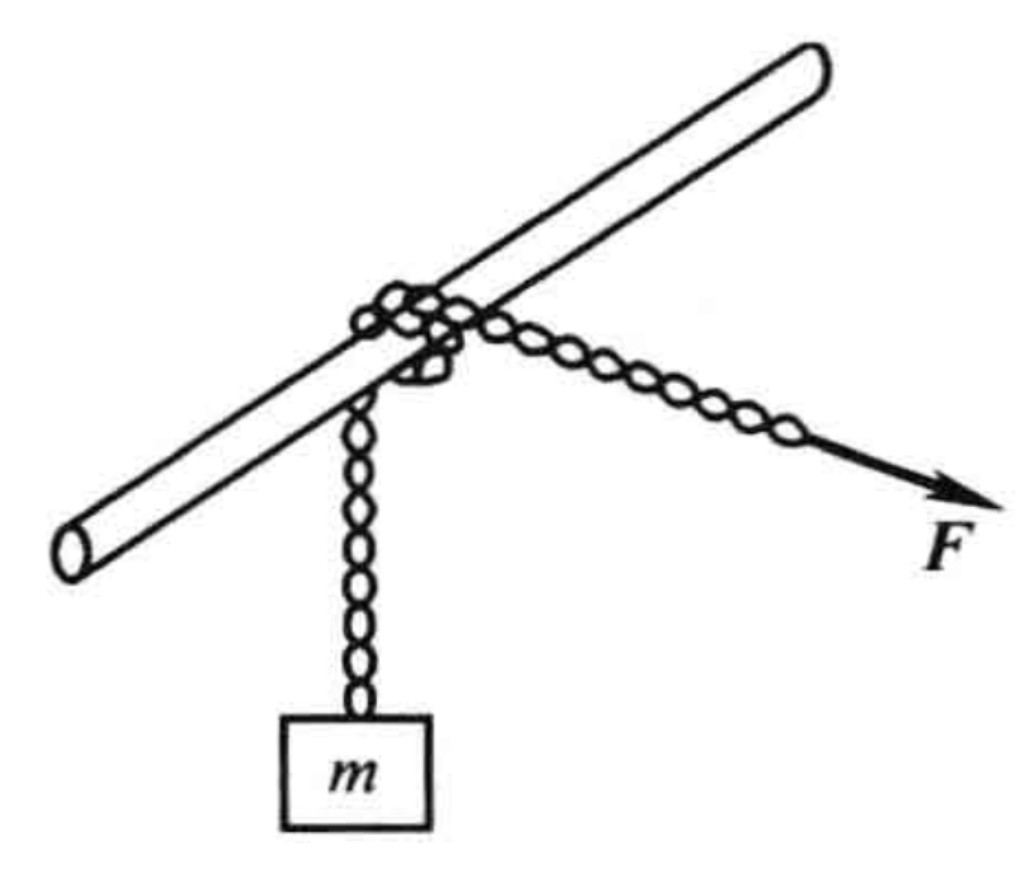
\includegraphics[width=0.3\textwidth]{figures/fig2-19_a.jpg}
  \end{figure}


\vfill

\textbf{2-20.}两物体的质量分别为 $m_0$ 和 $m$ , 用一根质量可以忽略的细绳相连, 细绳跨过装置在桌面上的定滑轮, 使物体 $m_0$ 放在光滑的桌面上, 而物体 $m$ 悬在桌边, 如习题 2-20 图所示。求物体 $m_0$ 运动的加速度。若将物体 $m$ 拿去, 而用大小为 $mg$ 的力向下拉绳, 则物体 $m_0$ 的加速度是否发生变化? 略去滑轮的质量和滑轮轴承处的摩擦力, 且细绳不能伸长。

\begin{figure}[H]
  \centering
  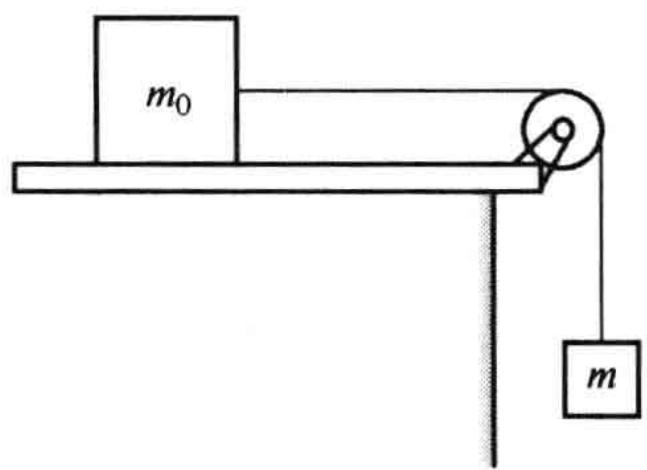
\includegraphics[width=0.3\textwidth]{figures/fig2-20.jpg}
  \end{figure}

\vfill
\newpage

\textbf{2-21.}一质量为 $50 \mathrm{~kg}$ 的人站在电梯里的台秤上, 求:

(1) 当电梯以 $4.9 \mathrm{~m} / \mathrm{s}$ 的速度匀速上升或下降时, 台秤读数各是多少?

(2) 当电梯以 $4.9 \mathrm{~m} / \mathrm{s}^{2}$ 的加速度上升或下降时, 台秤读数又各是多少?

\vfill

\textbf{2-22.}一飞机在竖直平面内以 $540 \mathrm{~km} / \mathrm{h}$ 的速度沿一圆周飞行。为使在飞机飞行过程中,驾驶员与座椅之间的相互作用力不大于驾驶员重力的 8 倍,试求此圆周的最小半径。

\vfill
\newpage

\textbf{2-23.}一质量为 $m$ 的物体静止于倾角为 $\theta$ 的固定斜面上, 如习题 2-23 图所示。已知物体与斜面间的静摩擦因数为 $\mu$ , 试问, 至少要用多大的力作用在物体上, 才能使它运动? 并指出该力的方向。

\begin{figure}[H]
  \centering
  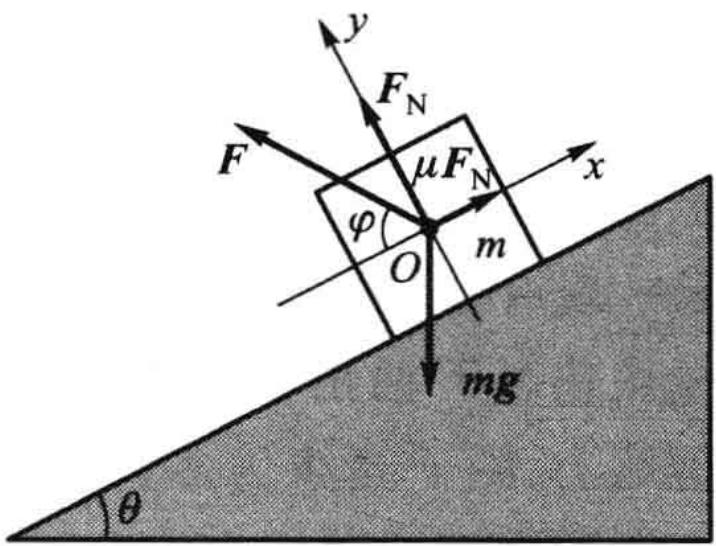
\includegraphics[width=0.25\textwidth]{figures/fig2-23.jpg}
  \end{figure}

\vfill

\textbf{2-24.}两个质量均为 $m$ 的质点 $A$ 和 $B$ 连在一个劲度系数为 $k$ 的弹簧的两端。开始两质点静止在光滑的水平面上,弹簧处于原长,然后沿 AB 方向给 B 以恒力 ka。求两质点的运动学方程。

\vfill
\newpage

\textbf{2-25.}质量为 $m_{0}$ 的木板静置在水平桌面上, 其一端与桌面对齐, 木板上放

一质量为 m 的小花瓶, 花瓶与板左端相距为 l, 桌面长为 L, 如习题 2-25 图所示。现有一水平恒力 F 作用于板上, 将板从花瓶下抽出。为使花瓶不至于掉落地上, 则 F 至少为多大? 设各接触面之间的摩擦因数均为 $\mu$ 。

\begin{figure}[H]
  \centering
  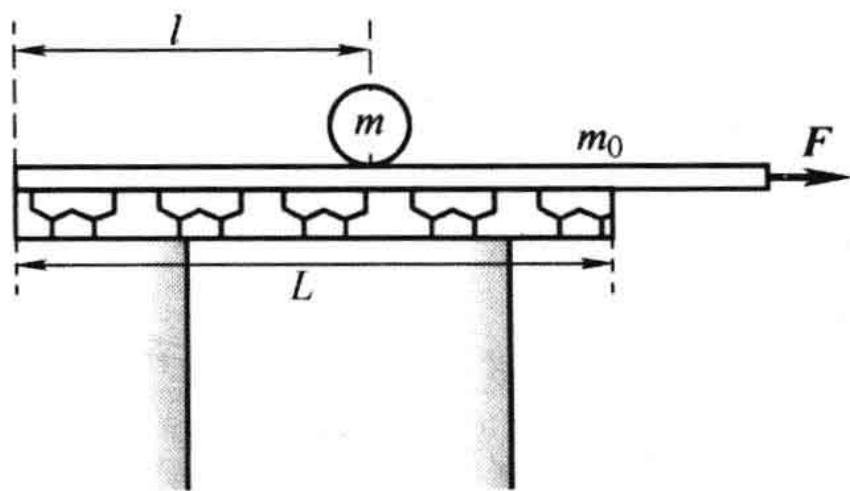
\includegraphics[width=0.3\textwidth]{figures/fig2-25.jpg}
  \end{figure}

\vfill

\textbf{2-26.}如习题 2-26 图所示, 质量分别为 $m_{1}$ 和 $m_{2} (m_{1} > m_{2})$ 的两物体叠放在水平桌面上, 另一质量为 $m_{3}$ 的物体通过细绳和滑轮组与 $m_{1}, m_{2}$ 相连并悬在桌边。

(1) 若 $m_{1}$ 与 $m_{2}$ 之间的摩擦因数为 $\mu$ ，而 $m_{1}$ 与桌面之间无摩擦力，求运动时， $m_{1}$ 与 $m_{2}$ 之间无相对滑动的条件；

(2) 若各接触面之间的摩擦因数均为 $\mu$ , 求 $m_{2}$ 与 $m_{3}$ 运动, 而 $m_{1}$ 保持静止的条件。

\begin{figure}[H]
  \centering
  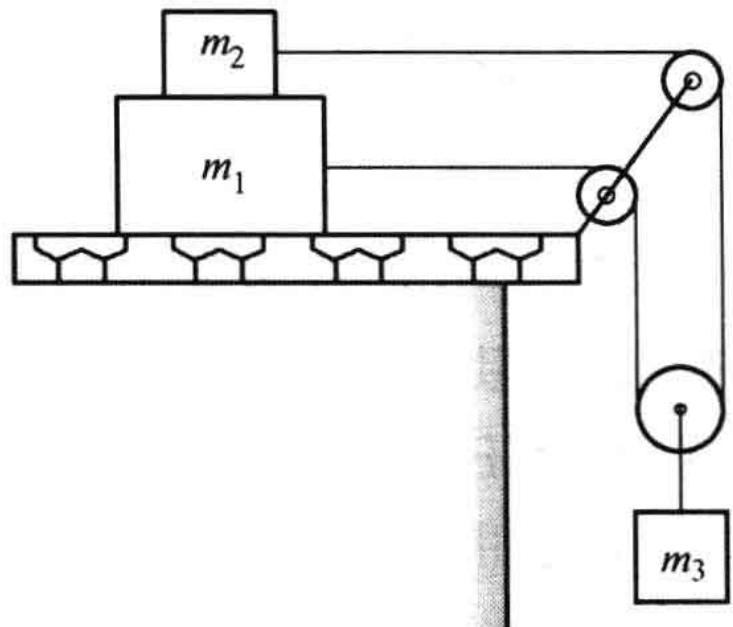
\includegraphics[width=0.25\textwidth]{figures/fig2-26.jpg}
  \end{figure}

\vfill
\newpage

\textbf{2-27.}空中有许多大小不等的雨滴(可看成圆球形)由静止开始下落。若受到的空气阻力 $F_{\mathrm{f}}$ 与其速度 $\nu$ 的一次方成正比, 即 $F_{\mathrm{f}} = -k\nu$ , 其中 $k$ 为常量。

(1) 求任一时刻 t 雨滴的速度 $v(t)$ ;

(2) 证明雨滴的速度最终将趋于一极限值 $v_{f}$ (称为终极速度), 并求出此 $v_{f}$ ;

(3) 若常量 $k$ 正比于各雨滴的大圆面积, 即 $k \propto \pi r^{2}$ ( $r$ 为雨滴的半径), 试问: 大、小雨滴中哪种雨滴获得的终极速度较大?

\vfill

\textbf{2-28.}一子弹以 $v_{0}$ 的初速度和 $\theta$ 仰角自地面射出, 子弹在飞行时受到的空气阻力为其速度的 $km$ 倍 ( $m$ 为子弹的质量, $k$ 为常量)。试求子弹的速度与水平线成 $45^{\circ}$ 角时, 子弹与发射点之间的水平距离 $s$ 。

\begin{figure}[H]
  \centering
  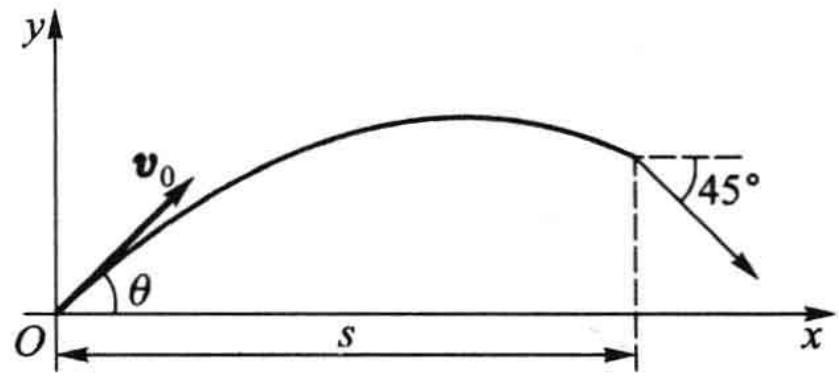
\includegraphics[width=0.3\textwidth]{figures/fig2-28.jpg}
\end{figure}

\vfill
\newpage

\textbf{3-1.}如习题 3-1 图所示,一小车沿倾角为 $\theta$ 的光滑斜面滑下。小车上悬挂一摆锤。当摆锤相对小车静止时,摆线与竖直线的夹角为多大?

\begin{figure}[H]
  \centering
  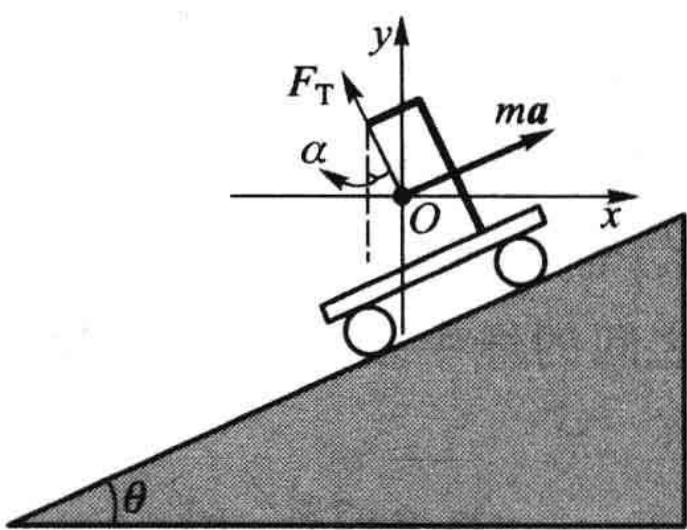
\includegraphics[width=0.25\textwidth]{figures/fig3-1_x.jpg}
  \end{figure}

\vfill

\textbf{3-2.}在卡车的尾部通过一根绳子拖着一根粗细均匀的圆木。绳长为 $d$ ，圆木长为 $l$ ，绳与卡车的连接点距地高 $h$ 。问卡车必须以多大的加速度 $a$ 行驶，才能使圆木与地面脱离？

\begin{figure}[H]
  \centering
  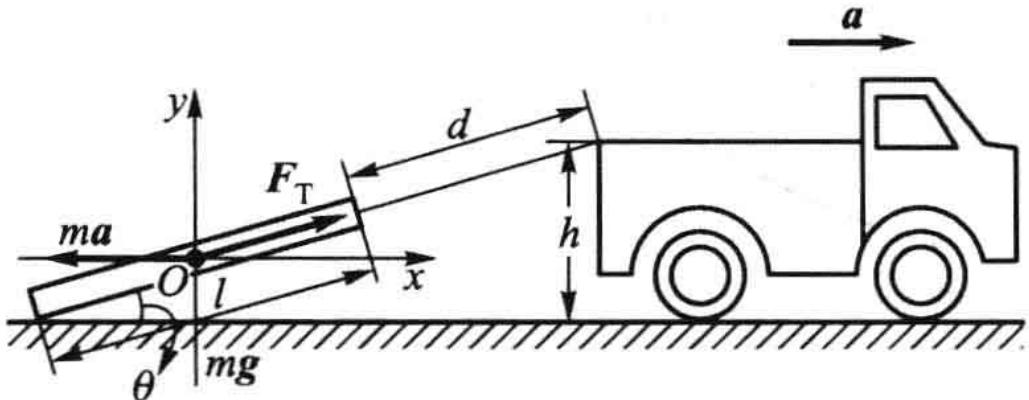
\includegraphics[width=0.4\textwidth]{figures/fig3-2.jpg}
  \end{figure}

\vfill
\newpage

\textbf{3-3.}在一体积为 $V$ , 质量为 $m_{0}$ 的铁盒内置有一阿特伍德机, 已知两物体的质量分别为 $m_{1}$ 和 $m_{2}$ 。现将此铁盒放入密度为 $\rho$ 的液体中, 如习题 3-3 图所示,试求铁盒在下沉过程中的加速度。忽略液体对铁盒的阻力作用。

\begin{figure}[H]
  \centering
  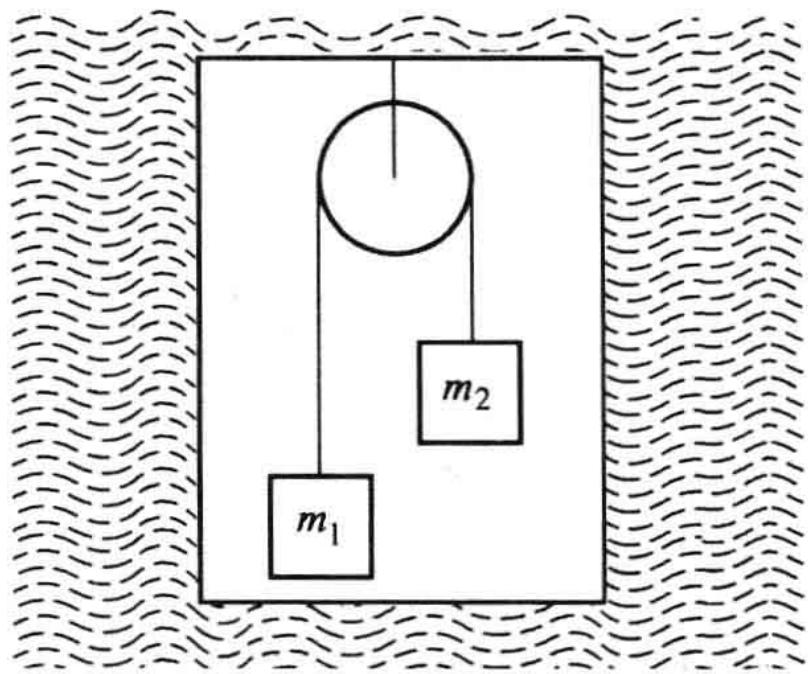
\includegraphics[width=0.25\textwidth]{figures/fig3-3.jpg}
  \end{figure}

\vfill

\textbf{3-4.}如习题 3-4 图所示, 质量为 $m_{2} = 2 \mathrm{~kg}$ 和 $m_{3} = 1 \mathrm{~kg}$ 的两个物体分别系在一根跨过滑轮 B 的细绳的两端, 而滑轮 B 又与质量为 $m_{1} = 3 \mathrm{~kg}$ 的物体系在另一根跨过定滑轮 A 的细绳的两端。试求:

(1) $m_{1}, m_{2}$ 和 $m_{3}$ 的加速度 $a_{1}, a_{2}$ 和 $a_{3}$ ;

(2) 跨过滑轮 A 的绳和跨过滑轮 B 的绳中张力 $F_{TA}$ 、 $F_{TB}$ 。

\vfill
\newpage

\textbf{3-5.}一质量为 $m_{0}$ , 倾角为 $\theta$ 的斜面体放在水平面上, 在斜面体上有一质量为 $m$ 的物体。为使 $m$ 不与斜面发生相对运动, 现用一水平力 $F$ 作用在 $m_{0}$ 上, 如习题 3-5 图所示。

(1) 若所有接触面均光滑, $F$ 应为多大?

(2) 若 $m$ 与 $m_0$ 之间的摩擦因数为 $\mu$ , 而 $m_0$ 与水平面间无摩擦, 求 $F$ 的范围。

\begin{figure}[H]
  \centering
  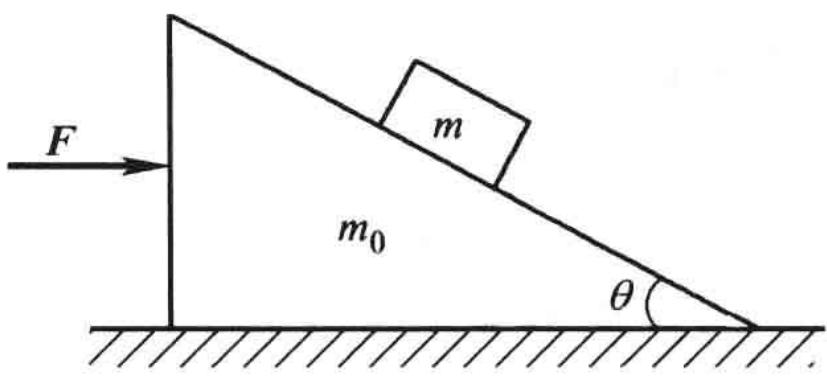
\includegraphics[width=0.4\textwidth]{figures/fig3-5.jpg}
  \end{figure}

\vfill

\textbf{3-6.}一摩托车以 $36 \mathrm{~km} / \mathrm{h}$ 的速率在地面上行驶。其轮胎与地面间的摩擦因数 $\mu$ 为0.3。试求：

(1) 摩托车在转弯时轨道的最小曲率半径;

(2) 摩托车与竖直线之间的最大倾斜角。

\vfill
\newpage

\textbf{3-7.}一根绳子的两端分别固定在顶板和底板上,两固定点位于同一竖直

线,相距为 $h$ 。一质量为 $m$ 的小球系于绳上某点处,当小球两边的绳均被拉直时,两绳与竖直线的夹角分别为 $\theta_{1}$ 和 $\theta_{2}$ ,如习题3-7图所示。当小球以一定的速度在水平面内做匀速圆周运动时,两绳均被拉直。试问:

(1) 若下面的绳子中的张力为零, 则小球的速度为多大?

(2) 若小球的速度是(1)小题中求得的速度的 $\sqrt{2}$ 倍, 则上、下两段绳中的张力各为多大?

\begin{figure}[H]
  \centering
  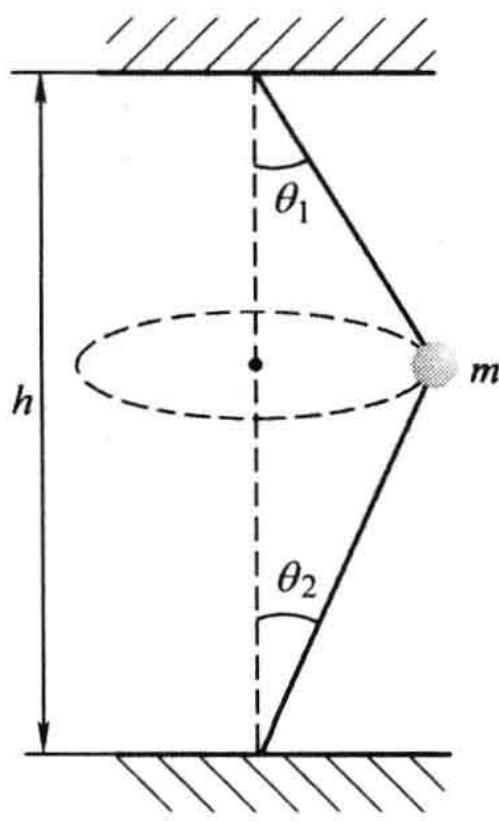
\includegraphics[width=0.2\textwidth]{figures/fig3-7.jpg}
  \end{figure}

\vfill

\textbf{3-8.}一小物体放在一半径为 $R$ 的水平圆盘边缘上, 小物体与圆盘间的静摩擦因数为 $\mu$ 。若圆盘绕其轴的角速度逐渐增大到一个值时, 小物体滑出圆盘并最终落到比盘面低 $h$ 的地面上。问从它离开圆盘的那一点算起, 小物体越过的水平距离多大?

\vfill
\newpage

\textbf{3-9.}一根光滑的钢丝弯成如习题3-9图所示的形状, 其上套有一小环。当钢丝以恒定角速度 $\omega$ 绕其竖直对称轴旋转时, 小环在其上任何位置都能相对静止。求钢丝的形状 (即写出 $y$ 与 $x$ 的关系)。

\begin{figure}[H]
  \centering
  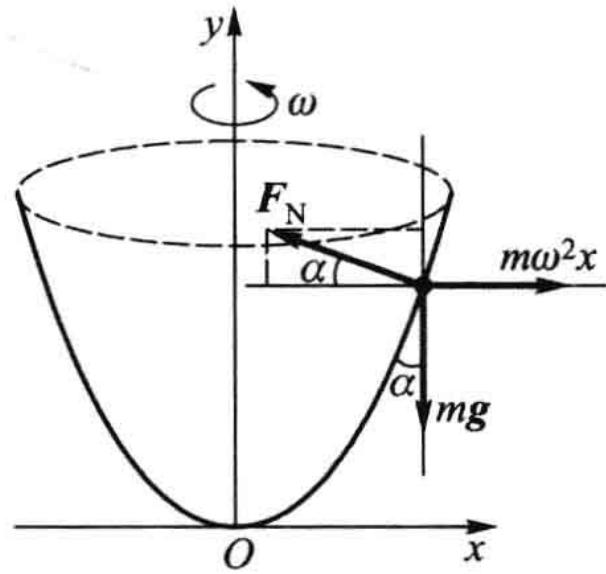
\includegraphics[width=0.3\textwidth]{figures/fig3-9.jpg}
  \end{figure}

\vfill

\textbf{3-10.}一圆盘绕其竖直的对称轴以恒定的角速度 $\omega$ 旋转。在圆盘上沿径向开有一光滑小槽, 槽内一质量为 $m$ 的质点以 $v_{0}$ 的初速从圆心开始沿半径向外运动。试求:

(1) 质点到达习题 3-10 图所示位置 (即 $y = y_0$ ) 时相对圆盘的速度 $v$ ;

(2) 质点到达该处所需要的时间 t;

(3) 质点在该处所受到的槽壁对它的侧向作用力 $F$ 。

\begin{figure}[H]
  \centering
  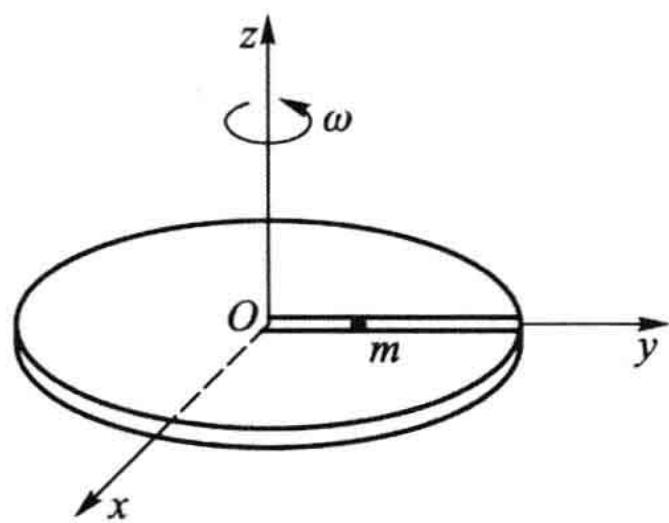
\includegraphics[width=0.3\textwidth]{figures/fig3-10.jpg}
  \end{figure}

\vfill
\newpage


\textbf{3-11.}在如习题 3-11 图所示的装置中, 质量分别为 $m_{2}$ 和 $m_{3}$ 的两物体由一细绳相连。细绳跨过装在一质量为 $m_{1}$ 的大物体上的定滑轮。已知所有的表面都光滑。试问:

(1) $m_{1}$ 的加速度为多大?

(2) 若在 $m_{1}$ 上作用一水平力 F，使 $m_{2}$ 和 $m_{3}$ 相对 $m_{1}$ 静止，则 F 为多大？

\begin{figure}[H]
  \centering
  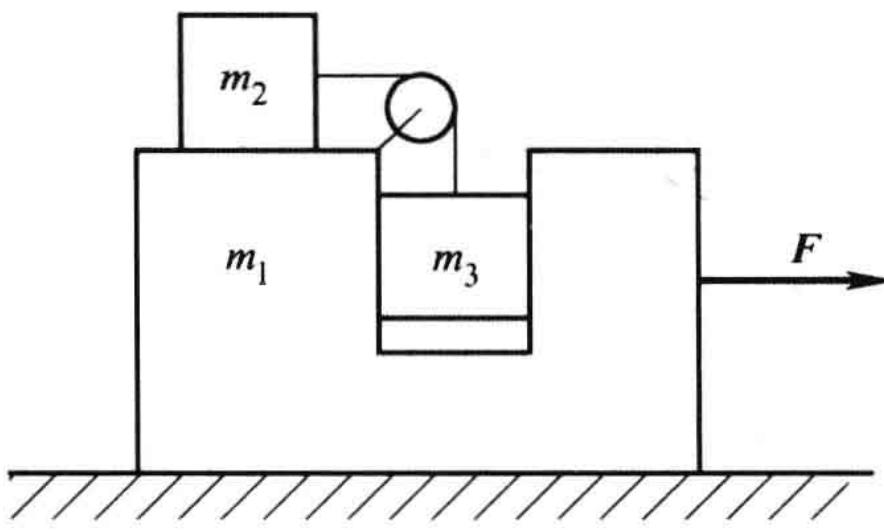
\includegraphics[width=0.3\textwidth]{figures/fig3-11_1.jpg}
  \end{figure}

\vfill

\textbf{3-12.}一个侧面边长比为 $3:4:5$ 的斜面固连在一转盘上, 如习题 3-12 图所示, 一木块静止在斜面上, 斜面和木块之间的摩擦因数 $\mu = \frac{1}{4}$ 。求此木块能保持在离转盘中心的水平距离为 $40 \mathrm{~cm}$ 处相对转盘不动的最小转动角速度 $\omega$ 。

\begin{figure}[H]
  \centering
  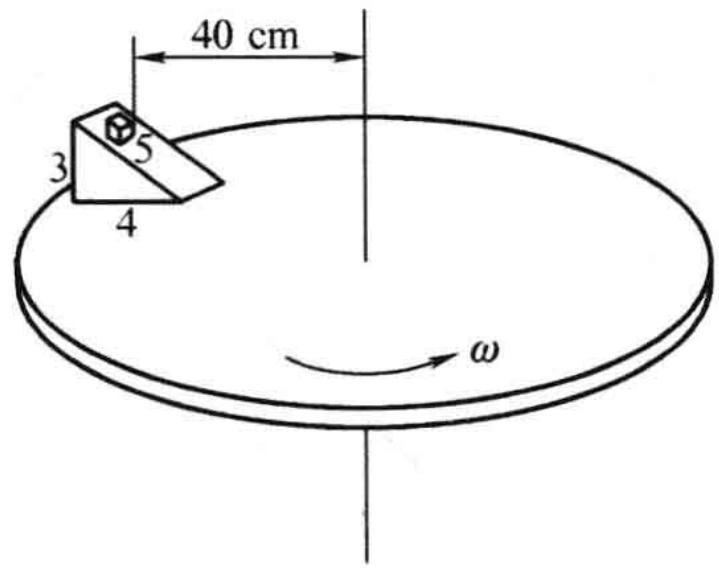
\includegraphics[width=0.25\textwidth]{figures/fig3-12.jpg}
  \end{figure}

\vfill
\newpage

\textbf{3-13.}一辆汽车驶入曲率半径为 $R$ 的弯道, 弯道倾斜一角度 $\theta$ , 车轮与路面之间的摩擦因数为 $\mu$ 。求汽车在路面上不侧向滑动时的最大和最小速度。

\vfill

\textbf{3-14.}一半顶角为 $\alpha$ 的竖直倒立圆锥面, 圆锥面以恒定的角速度 $\omega$ 绕其对称轴旋转。在圆锥内表面距轴为 $r$ 处有一质点。

（1）若圆锥面内表面光滑，要使质点随锥面一起匀速转动，即与锥面相对静止，求 $\omega$ 的值；

(2) 若质点与锥面间的摩擦因数为 $\mu$ , 为使质点相对锥面静止, 求 $\omega$ 的范围。

\vfill
\newpage

\textbf{3-15.}质量分别为 $m$ 及 $m'$ 的两个质点, 用未伸缩时长度为 $a$ 的弹性绳相连, 绳的劲度系数 $k = \frac{2mm' \omega^2}{m + m'}$ 。将此系统放在光滑的水平管内, 管子绕通过管上某点的竖直轴以恒定角速度 $\omega$ 转动。开始时, 两质点相对于管子是静止的, 两质点间距为 $a$ 。试求此后任何时刻两质点间的距离。

\vfill

\textbf{3-16.}质量为 $m$ 的小环套在半径为 $a$ 的光滑圆圈上, 可在其上滑动。如圆圈在水平面内以恒定角速度 $\omega$ 绕圈上某点 $O$ 转动, 转轴垂直于水平面, 如习题 3-16 图所示, 试求小环沿圆圈切线方向的运动微分方程。

\begin{figure}[H]
  \centering
  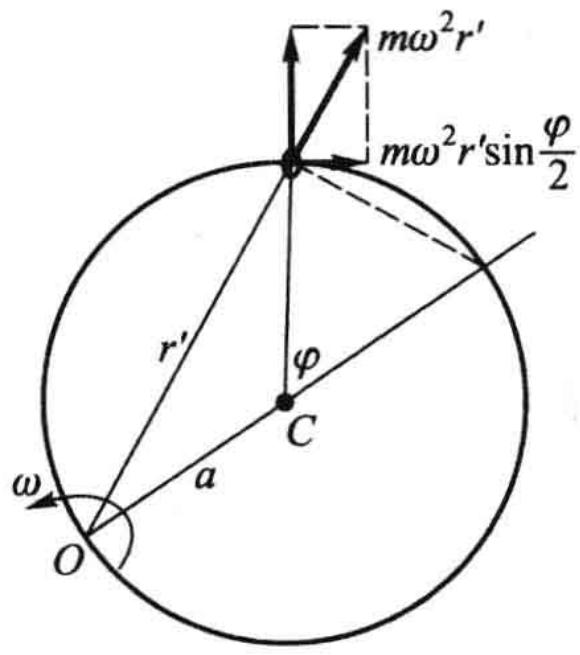
\includegraphics[width=0.25\textwidth]{figures/fig3-16.jpg}
  \end{figure}

\vfill
\newpage

\textbf{3-17.}质量为 $m$ 的小球置于光滑水平台面, 用长为 $l$ 的细绳系于台面上的 $P$ 点, 水平台面绕着过 $O$ 点的竖直轴以恒定角速度 $\omega$ 旋转, $P$ 点与 $O$ 点的距离为 $d$ 。试列出小球的运动方程。设在小球运动过程中, 绳始终保持拉直状态。

\begin{figure}[H]
  \centering
  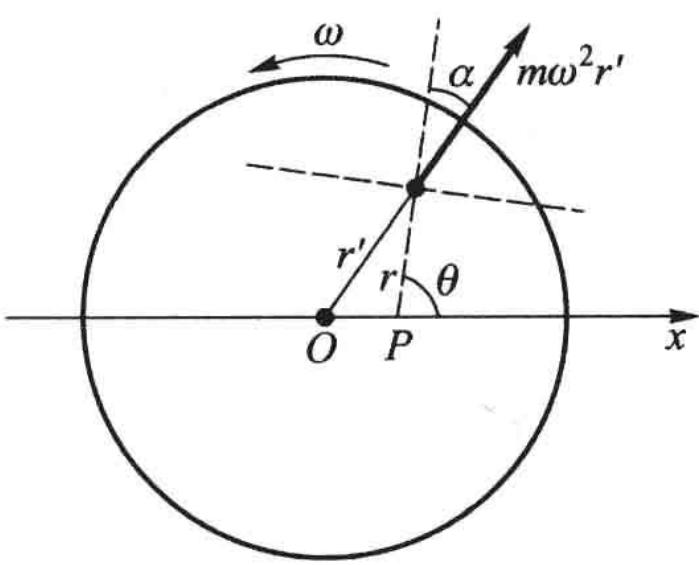
\includegraphics[width=0.3\textwidth]{figures/fig3-17.jpg}
  \end{figure}

\vfill

\textbf{3-18.}一圆柱形刚性杆 $OA$ 上套有一质量为 $m$ 的小环, 杆的一端固定, 整个杆绕着通过固定端 $O$ 的竖直轴以恒定的角速度旋转, 旋转时杆与竖直方向的夹角 $\alpha$ 保持不变。设小环与杆之间的摩擦因数为 $\mu$ , 已知当小环相对杆运动到习题 3-18 图所示的位置 $x$ 时, 其相对于杆的速度为 $\dot{x}$ , 试列出此时小环沿杆的运动方程。(不要求解出此方程)
\vfill
\newpage

\textbf{4-1.}地球的质量是月球的 81 倍。地球和月球的中心相距 $3.84 \times 10^{8} \mathrm{~m}$ , 求地球和月球组成的系统的质心与地球中心的距离。

\begin{figure}[H]
  \centering
  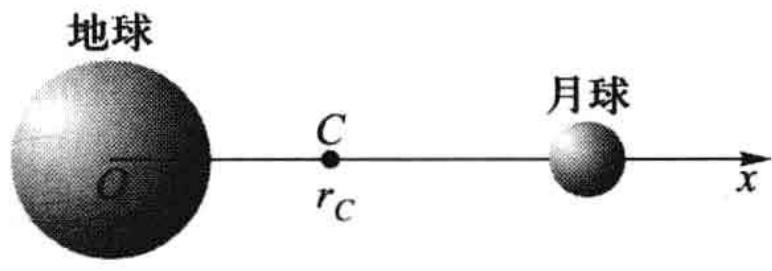
\includegraphics[width=0.4\textwidth]{figures/fig4-1.jpg}
  \end{figure}

\vfill

\textbf{4-2.}$A 、 B 、 C$ 三质点在某一时刻的位置坐标分别为: $(-3, 4, 3)$ 、 $(3, -8, 6)$ 、 $(1, 2, -1)$ , 坐标以 $\mathrm{m}$ 为单位, $B$ 的质量是 $A$ 的两倍, 而 $C$ 的质量是 $A$ 的三倍。求此时由此三质点组成的体系的质心的位置。

\vfill
\newpage

\textbf{4-3.}长为 $l$ 、线密度为 $\rho_{l}$ 的柔软绳索, 原先两端点 $A 、 B$ 并合一起, 悬挂在支点上, 现让 $B$ 端脱离支点自由下落, 求当 $B$ 端下落了 $x$ 时, 支点上所受的力 $F_{\mathrm{T}}$ 。

\begin{figure}[H]
  \centering
  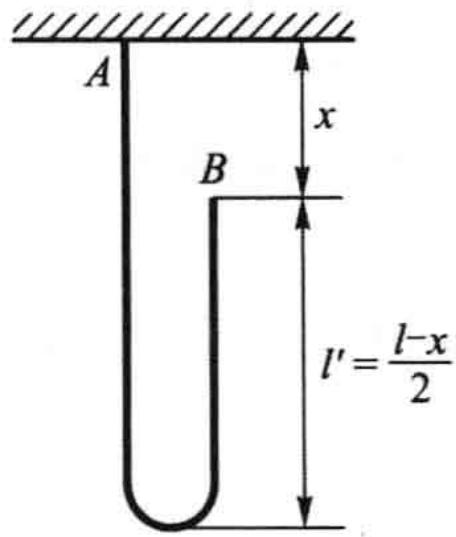
\includegraphics[width=0.2\textwidth]{figures/fig4-3.jpg}
  \end{figure}

\vfill

\textbf{4-4.}如习题 4-4 图所示, 光滑水平面上并排静放着两块质量分别为 $m_{1}$ 和

$m_{2}$ 的木块。一质量为 m 的子弹以初速度 $v_{0}$ 水平射向两木块，射穿两木块后以 $v'$ 的速度沿原方向运动。求两木块的速度 $v_{1}$ 和 $v_{2}$ 。设子弹在两木块中受到的阻力（可视为恒力）相等，而穿过 $m_{1}$ 所用的时间为穿过 $m_{2}$ 所用时间的一半。

\begin{figure}[H]
  \centering
  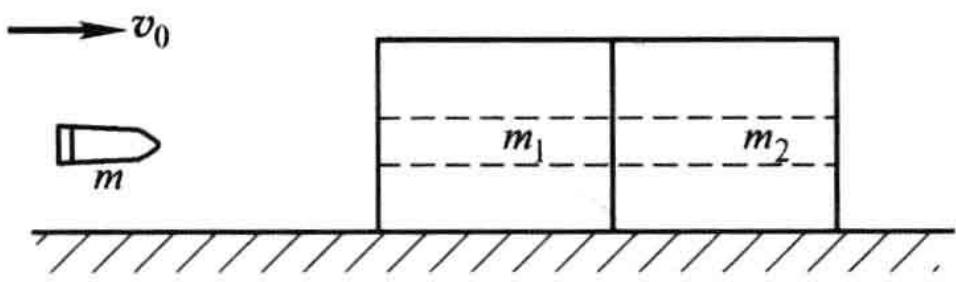
\includegraphics[width=0.4\textwidth]{figures/fig4-4.jpg}
  \end{figure}

\vfill
\newpage

\textbf{4-5.}一块长为 $L$ 的大平板静放在光滑水平冰面上, 一小孩骑着儿童自行车以 $v_{0}$ 的速度从板的一端驶上平板, 在板上他的速度忽快忽慢, 在将近板的另一端时, 他相对板的速度为 $u$ 。此时, 他忽然刹车, 在板的另一端边缘车相对板静止。已知人在板上骑车的时间为 $t$ , 板的质量为 $m_{0}$ , 小孩与车一起的质量为 $m$ 。试求:

(1) 刹车前瞬时板的速度;

(2) 车相对板刚静止时板的位移。

\vfill

\textbf{4-6.}两个质量分别为 $m_{1}$ 和 $m_{2} (m_{1} > m_{2})$ 的人身高相同, 他们同时以相同的速率竖直上跳, 在空中二人用力互推。若胖人的落地点距起跳点为 $s$ , 则瘦人的落地点距起跳点多远?

\vfill
\newpage

\textbf{4-7.}质量为 $m_{0}$ , 长为 $l$ 的小船静浮于河中, 小船两头分别站着质量为 $m_{1}$ 和

$m_{2}(m_{1}>m_{2})$ 的人,他们同时相对船以相同的速率 u 走向原位于船正中,但固定在河中的木桩,如习题 4-7 图所示。若忽略水对船的阻力作用,试问:

(1) 谁先走到木桩处?

(2) 他用了多少时间？

\begin{figure}[H]
  \centering
  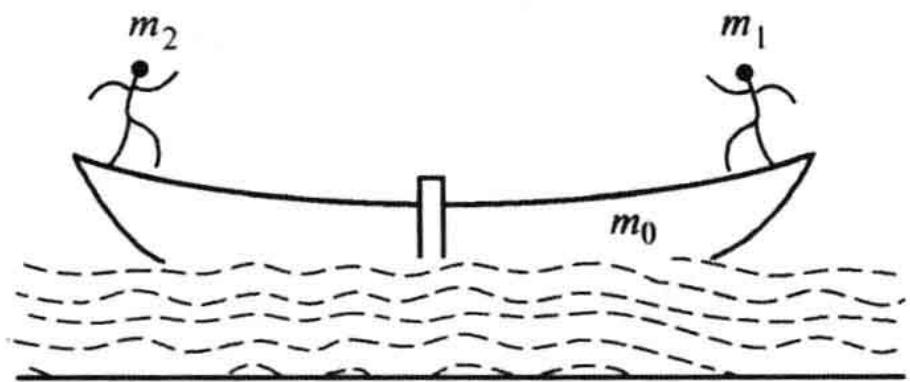
\includegraphics[width=0.3\textwidth]{figures/fig4-7.jpg}
  \end{figure}

\vfill

\textbf{4-8.}一质量为 $m_{1}$ 的杂技演员, 从蹦床上沿竖直方向跳起。当他上升到某一高度时, 迅速抱起边上栖木上的质量为 $m_{2}$ 的猴子, 结果他又上升了相同的高度然后落下。试求此种情况下杂技演员所能上升的高度 $h$ 与他不抱猴子所能达到的最大高度 $h_{0}$ 之比。

\vfill
\newpage

\textbf{4-9.}一火箭竖直向上发射, 当它达到最高点时炸裂成三个等质量的碎片, 观察到其中一块碎片经时间 $t_1$ 竖直地落到地上, 而其他两块碎片在炸裂后的 $t_2$ 时刻落在地上, 求火箭炸裂时离地面的高度。

\vfill

\textbf{4-10.}将一空盒放在秤盘上,并将秤的读数调整到零,然后从高出盒底 $h$ 处将小钢珠以每秒 $B$ 个的速率由静止开始掉入盒内,每一小钢珠的质量为 $m$ 。若钢珠与盒底碰撞后即静止,忽略小球在空中的时间,试求自钢珠落入盒内起,经过时间 $t$ 后秤的读数。

\vfill
\newpage

\textbf{4-11.}由喷泉中喷出的水柱, 把一个质量为 $m$ 的垃圾桶倒顶在空中。水以恒定的速率 $v_{0}$ 从面积为 $S$ 的小孔中喷出, 射向空中, 在冲击垃圾桶桶底以后, 有一半的水吸附在桶底, 并顺内壁流下, 其速度可忽略, 而另一半则以原速竖直溅下。求垃圾桶停留的高度 $h$ 。

\vfill

\textbf{4-12.}一质量为 $m_{0}$ (无水时) 的水桶开始时处于静止状态, 桶中装有质量为 $m$ 的水, 通过一根绳子施以恒力 $F$ 将桶从井中提上来, 桶中的水以恒定的质量速率从桶中漏出来, 经过时间 $t$ 桶变成空的。求变成空桶的瞬间桶的速度。

\vfill
\newpage

\textbf{4-13.}求均质的内外半径分别为 $a$ 和 $b$ 的半球壳的质心。

\vfill

\textbf{4-14.}在光滑的水平面上有两个质量分别为 $m_{1}$ 和 $m_{2}$ 的物体。它们中间用

一根原长为 l，劲度系数为 k 的弹簧相连，如习题 4-14 图所示。开始时，将 $m_{1}$ 紧靠墙，并将弹簧压缩至原长的 $\frac{1}{2}$ ，然后将 $m_{2}$ 释放。若以 $m_{1}$ 、 $m_{2}$ 和弹簧为系统，试求：

(1) 系统质心的加速度随时间的变化关系;

(2) 系统质心的速度最大值。

\begin{figure}[H]
  \centering
  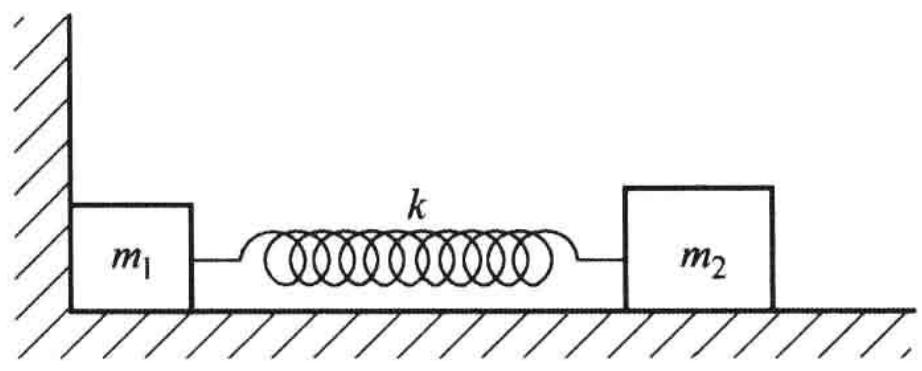
\includegraphics[width=0.4\textwidth]{figures/fig4-14_1.jpg}
  \end{figure}

\vfill
\newpage

\textbf{4-15.}一圆锥摆的摆线长为 $l$ , 摆锤的质量为 $m$ , 圆锥的半顶角为 $\alpha$ 。试求当摆锤从习题 4-15 图中位置 $A$ 沿圆周匀速运动到位置 $B$ 的过程中张力的冲量。

\begin{figure}[H]
  \centering
  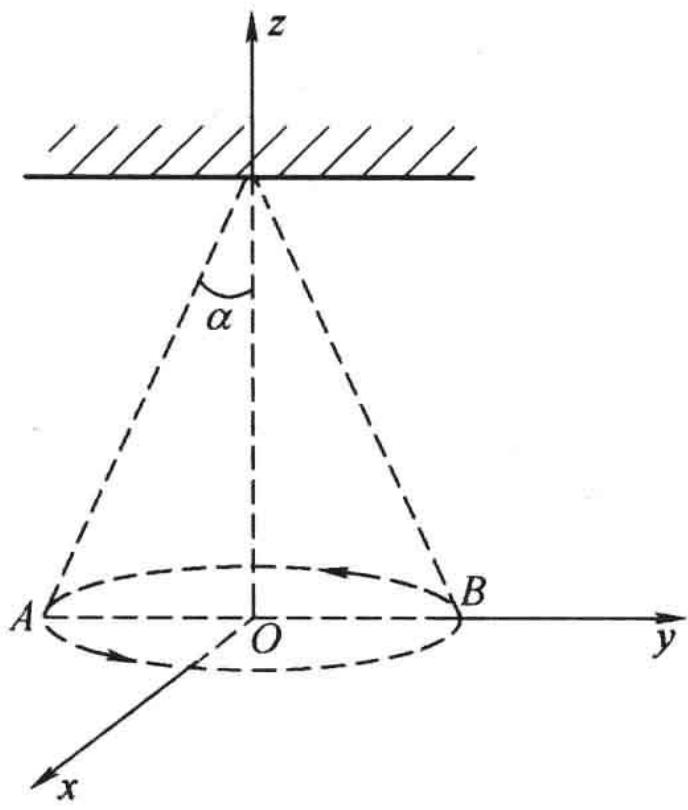
\includegraphics[width=0.3\textwidth]{figures/fig4-15.jpg}
  \end{figure}

\vfill

\textbf{4-16.}两质量皆为 $m_0$ 的冰车头尾相接地静止在光滑的水平冰面上。一质量为 $m$ 的人从一车跳到另一车, 然后再跳回。试证明: 两冰车的末速度之比为 $\frac{m_0 + m}{m_0}$ 。

\vfill
\newpage

\textbf{4-17.}如习题 4-17 图所示, 质量为 $m$ 的物体从静止下落 $y$ 后开始拉起质量为 $m_{0}(m_{0}>m)$ 的物体。两物体通过一根很轻且不可伸长的细绳相连并挂在一固定的光滑滑轮上。(1) 求物体 $m_{0}$ 返回原来位置所用的时间; (2) 求物体 $m_{0}$ 被拉起运动时系统减少的动能与原动能的比值。

\begin{figure}[H]
  \centering
  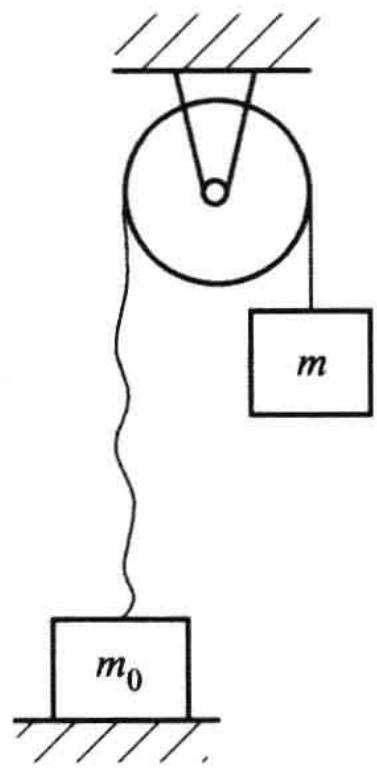
\includegraphics[width=0.18\textwidth]{figures/fig4-17.jpg}
  \end{figure}

\vfill

\textbf{4-18.}质量为 $m_{0}$ 的人手里拿着一个质量为 $m$ 的物体, 以 $v_{0}$ 的初速度向与地平线成 $\alpha$ 角的方向跳去, 当他达到最高点时, 将物体以相对速度 $u$ 水平向后抛出。问由于物体的抛出, 人向前跳出的距离增加了多少?

\vfill
\newpage

\textbf{4-19.}一质量为 $m$ 的男孩站在质量为 $m_0$ 的雪橇上以恒定的速度 $v_i$ 在冰面上滑行。若男孩沿与 $v_i$ 相反的方向在雪橇上跑动, 在离开雪橇末端时相对于雪橇的速率为 v。求雪橇相对于冰面的末速度。

\vfill

\textbf{4-20.}有 $N$ 个人站在铁路上静止的质量为 $m_0$ 的平板车上, 每人的质量均为 $m$ 。他们以相对于平板车的速度 $u$ 跳离平板车。设平板车与轨道间无摩擦力。

(1) 若所有的人同时跳,则平板车的最终速度是多少?

(2) 若他们一个一个地跳, 则平板车的最终速度是多少?

(3) 以上两种情况中哪一种的最终速度大些?

\vfill
\newpage

\textbf{4-21.}一质量 $m_{1} = 50 \mathrm{~kg}$ 的人 A 手里拿着一质量 $m = 5.0 \mathrm{~kg}$ 的小球以 $v_{1} = 1.2 \mathrm{~m} / \mathrm{s}$ 的速率在光滑冰面上沿直线滑冰, 而另一质量 $m_{2} = 45 \mathrm{~kg}$ 的人 B 以 $v_{2} = 0.8 \mathrm{~m} / \mathrm{s}$ 的速率向 A 对面滑来, 为避免碰撞, A 把球以相对于他的速率 $u$ 向 B 水平抛去, 让 B 接住。试问 $u$ 至少应多大?

\vfill

\textbf{4-22.}质量为 $m_{\mathrm{A}}$ 与 $m_{\mathrm{B}}$ 的两个小球 $\mathrm{A}$ 和 $\mathrm{B}$ , 用不可伸长的轻绳相连, 静止在水平面上。绳子拉紧时, 给 $\mathrm{B}$ 球一个冲量 $\mathbf{I}$ ,

I 的方向与 AB 连线成 $\alpha$ 角, $\alpha < \frac{\pi}{2}$ , 如习题 4-22 图所示。已知冲击后的速度 $v_{B}$ 的大小, 求 $v_{B}$ 的方向和冲量 I 的大小。

\begin{figure}[H]
  \centering
  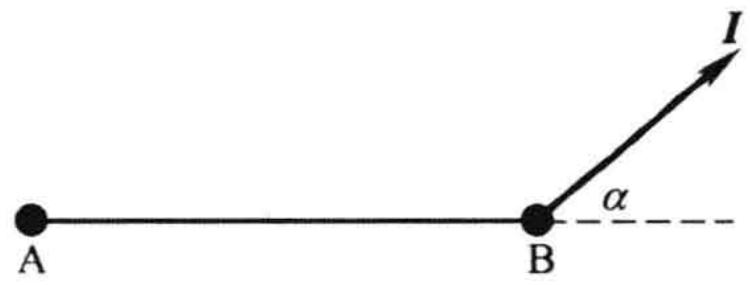
\includegraphics[width=0.4\textwidth]{figures/fig4-22.jpg}
  \end{figure}

\vfill
\newpage

\textbf{4-23.}如习题 4-23 图所示, 漏斗中的煤粉不断地落到速度 $v = 1.5 \mathrm{~m} / \mathrm{s}$ 的自动传送带上, 每秒钟落下的煤粉量为 $20 \mathrm{~kg}$ 。求煤粉作用在传送带上的水平方向的力。

\begin{figure}[H]
  \centering
  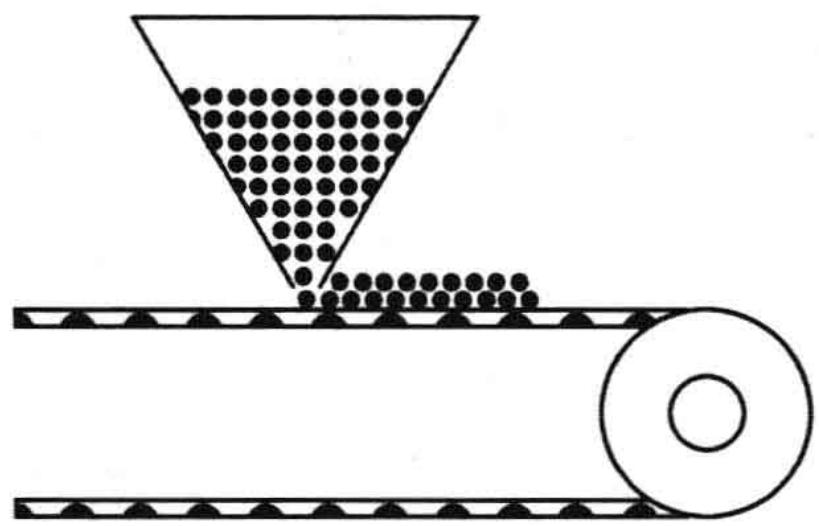
\includegraphics[width=0.25\textwidth]{figures/fig4-23.jpg}
  \end{figure}

\vfill

\textbf{4-24.}一股横截面积为 $S$ 、密度为 $\rho$ 、以绝对速度 $v_{0}$ 在水平方向运动的水流,无弹性地射中一静止在水平面上、质量为 $m$ 的木块,水离开木块时相对于木块的水平速度分量为零。若木块与它在其上滑动的水平面间的摩擦因数为 $\mu$ ,求木块的最终速度。

\vfill
\newpage

\textbf{4-25.}某人用木桶从深井中打水。木桶的质量为 $m_0$ ，刚开始提桶 $(t = 0)$ 时，桶内装有质量为 $m$ 的水，由于桶的底部有一面积为 $S$ 的小洞，桶内的水以相对于桶的恒定速率 $u$ 从洞口流出。

(1) 若人以恒定的速率向上提桶, 求提桶力随时间的变化关系;

(2) 若人以恒力 $F$ 向上提桶, 求水桶在时刻 $t$ 的速率。设 $t = 0$ 时桶静止。

\vfill

\textbf{4-26.}质量为 $m$ 的卡车关闭发动机后在雨中行驶。雨水以速率 $B(\mathrm{kg/s})$ 竖直滴进敞开的车厢内。设 $t = 0$ 时, 车厢是空的, 车速为 $v_{0}$ , 车厢内总共可容纳质量为 $m_{0}(\mathrm{kg})$ 的水。忽略地面对卡车的阻力作用, 试求卡车的速率随时间的变化关系 ( $t$ 从 0 到 $\infty$ )。

\vfill
\newpage

\textbf{4-27.}两质量分别为 $m_{1}$ 和 $m_{2}$ 的小车 A、B 尾尾相接地停在水平路面上, 如习题 4-27 图所示。两车之间用粗绳连接, A 车上装有质量为 $m$ 的水。在 $t = 0$ 时, B 车开始受到一水平恒力 $F$ 的作用, 而 A 车开始以相对于自身的速率 $u$ 把水水平地喷向 B 车, 并全部进入 B 车。设水柱的横截面积为 $S$ , 并忽略地面对两车的阻力作用。试求绳中张力随时间的变化关系。忽略在空中飞行的水柱。

\begin{figure}[H]
  \centering
  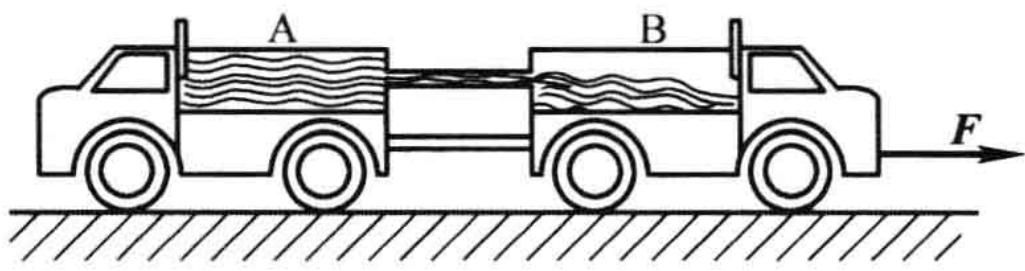
\includegraphics[width=0.4\textwidth]{figures/fig4-27.jpg}
  \end{figure}

\vfill

\textbf{4-28.}若上题中两车之间没有粗绳连接: (1) 在 A 车喷水以后, B 车在外力作用下始终与 A 车保持一定的距离。试求此外力随时间的变化关系; (2) 若两车均无外力作用, 试求在水不能喷入 B 车以前, A、B 两车的速度随时间的变化关系。

以上两小题均忽略地面对车的阻力作用,并可忽略在空中飞行的水柱。

\vfill
\newpage

\textbf{4-29.}如习题 4-29 图所示,一质量为 $m$ 的物体与单位长度的质量为 $\rho_{l}$ 的软绳相连。开始时,物体静置于倾角为 $\theta$ 的光滑斜面的顶端,而软绳则盘放在斜面顶端边的平台上。释放物体,让其沿斜面滑下。求当它下滑距离 x 时的速度。

\begin{figure}[H]
  \centering
  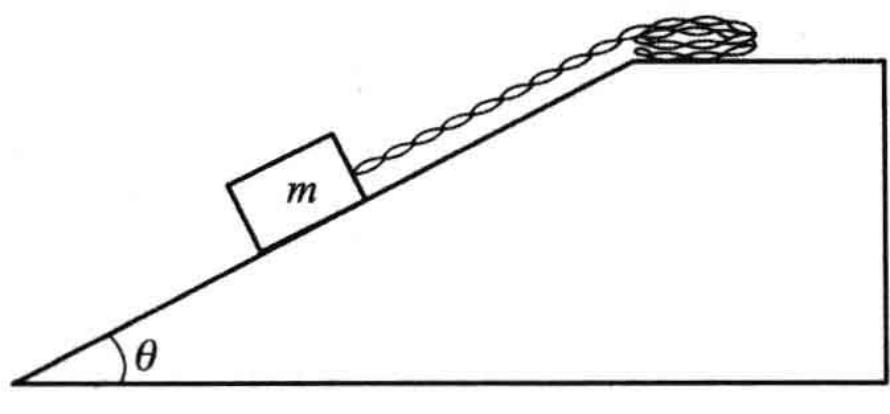
\includegraphics[width=0.3\textwidth]{figures/fig4-29.jpg}
  \end{figure}

\vfill

\textbf{4-30.}线密度为 $\rho_{l}$ 的柔软长链条盘成一团置于地面, 链条的一端系着一质量为 $m$ 的球, 若将球以初速 $v_{0}$ 竖直上抛, 球能上升至多高?

\vfill
\newpage

\textbf{4-31.}从地面发射质量为 $m$ 的火箭（包括燃料），其喷射的燃料气体相对火箭的速度为 $v_{\mathrm{r}}$ ，经过时间 $t_0$ 后，燃料全部喷射完，此时火箭正好获得逃逸速度。设在燃料喷射过程中重力加速度 $g$ 为常量。求空火箭的质量 $m_0$ 。

\vfill

\textbf{4-32.}从地面发射一初始质量为 $m_0$ 的火箭, 喷射的燃料相对火箭的速度为 $v_r$ 。(1) 若其燃料的每秒消耗量 $\frac{\mathrm{dm}}{\mathrm{dt}}$ 可调节, 为使火箭在地面以上某个高度保持静止, 求 $\frac{\mathrm{dm}}{\mathrm{dt}}$ 与时间 $t$ 的函数关系。(2) 若其燃料的每秒消耗量 $\frac{\mathrm{dm}}{\mathrm{dt}}$ 正比于火箭的瞬时质量 $m$ , 即 $\frac{\mathrm{dm}}{\mathrm{dt}} = -\alpha m$ , 其中 $\alpha$ 为正常量。证明当 $\alpha v_r > g$ 时, 火箭将以恒定加速度向上加速, 并求出此加速度。(3) 若其燃料的每秒消耗量 $\frac{\mathrm{dm}}{\mathrm{dt}}$ 正比于 $m_0$ , 即$\frac{\mathrm{d}m}{\mathrm{d}t} = -km_0$ ，其中 $k$ 为正常量。试求火箭在任一时刻 $t$ 的速度。（4）在（3）的情况下，若火箭本身的质量为 $m$ ，试求火箭所能到达的最大高度（不计火箭燃料燃尽后的自由上抛过程）。设火箭到达最大高度时仍未脱离地球引力范围，并设此过程中重力加速度 $g$ 为常量。

\vfill
\newpage

\textbf{4-33.}一火箭总质量为 $m$ , 其中机壳重为 $\beta m$ , 每秒喷出燃料 $\alpha m$ ( $\alpha$ 为常量)。为使火箭在开始喷射燃料的瞬时即能竖直起飞, 燃料的喷射速度 (相对火箭) $v_{r}$ 至少为多大? 维持用这样的速度喷射燃料, 当燃料恰好喷射完时, 火箭上升的最大高度 $h$ 为多少? 设重力加速度 $g$ 为常量。

\vfill
\newpage

\textbf{5-1.}光滑水平面上并排静放着两块质量分别为 $m_{1}$ 和 $m_{2}$ 的木块。一质量为 $m$ 的子弹以 $v_{0}$ 的初速度水平地射向两木块，若 $m_{1} = 2m_{0}, m_{2} = m_{0}$ ，质量为 $m$ 的子弹水平射穿 $m_{1}$ 后，射入 $m_{2}$ 内。当子弹相对 $m_{2}$ 静止时， $m_{2}$ 的速度是 $m_{1}$ 的两倍。求此过程中摩擦阻力所做的功。

\vfill

\textbf{5-2.}汽车沿着一坡度不大的斜坡以 $v_{1} = 12 \mathrm{~m} / \mathrm{s}$ 的速率向上匀速行驶, 当此车用同样的功率沿斜坡向下匀速行驶时, 车速为 $v_{2} = 20 \mathrm{~m} / \mathrm{s}$ 。若此车保持功率不变而沿同样的水平路面以匀速 $v$ 行驶, 设汽车在水平路面上受到的阻力与在斜坡上受到的阻力相同, 求 $v$ 的大小。

\vfill
\newpage

\textbf{5-3.}一质点在保守力场中沿 $x$ 轴（在 $x > 0$ 范围内）运动，其势能为 $E_{\mathrm{p}} = \frac{kx}{x^{2} + a^{2}}$ 。式中 $k, a$ 均为大于零的常量。试求：

(1) 质点所受到的力的表示式;

(2) 质点的平衡位置；

(3) 若质点静止在平衡位置,试讨论平衡的稳定性。

\vfill

\textbf{5-4.}一块长为 $l$ , 质量为 $m_{0}$ 的木板静置于光滑的水平桌面上, 在板的左端有一质量为 $m$ 的小物体 (大小可忽略) 以 $v_{0}$ 的初速度相对板向右滑动, 当它滑至板的右端时相对板静止。试求:

(1) 物体与板之间的摩擦因数;

(2) 在此过程中板的位移。

\vfill
\newpage

\textbf{5-5.}在倾角为 $\theta$ 的斜面上, 一质量为 $m$ 的物体通过一劲度系数为 $k$ 的弹簧与固定在斜面上的挡板相连, 如习题 5- 5 图所示。物体与斜面间的摩擦因数为

$\mu$ 。开始时，m 静止，弹簧处于原长。现有一沿斜面向上的恒力 F 作用在 m 上，使 m 沿斜面向上滑动。试求：从 m 开始运动到它运动到最高位置过程中力 F 所做的功。

\begin{figure}[H]
  \centering
  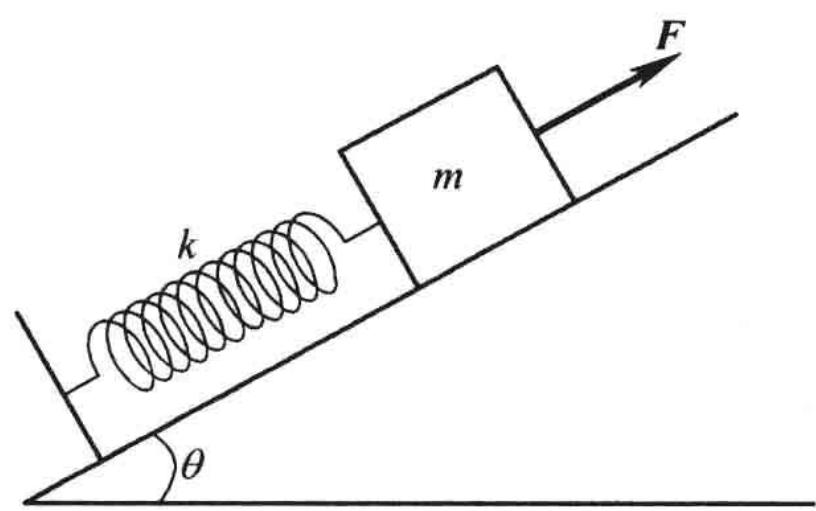
\includegraphics[width=0.3\textwidth]{figures/fig5-5.jpg}
  \end{figure}

\vfill

\textbf{5-6.}一小球做竖直上抛运动, 当它回到抛出点时, 速度为抛出时的 $3 / 4$ 。设小球运动中受到的空气阻力为恒力。试求:

(1) 小球受到的空气阻力与重力之比;

(2) 小球上升的最大高度与真空情况下最大高度之比 $(g = 10 \mathrm{~m} / \mathrm{s}^{2})$ 。

\vfill
\newpage

\textbf{5-7.}如习题 5-7 图所示, 质量为 $m$ 的物体以 $v_{0}$ 的速度在光滑水平面上沿 $x$ 轴正方向运动, 当它到达原点 $O$ 时, 撞击一劲度系数为 $k$ 的轻弹簧, 并开始受到摩擦力的作用,摩擦因数是位置的函数,可表示为 $\mu = ax$ (a 为一较小的常量)。求物体第一次返回 O 点时的速度。

\begin{figure}[H]
  \centering
  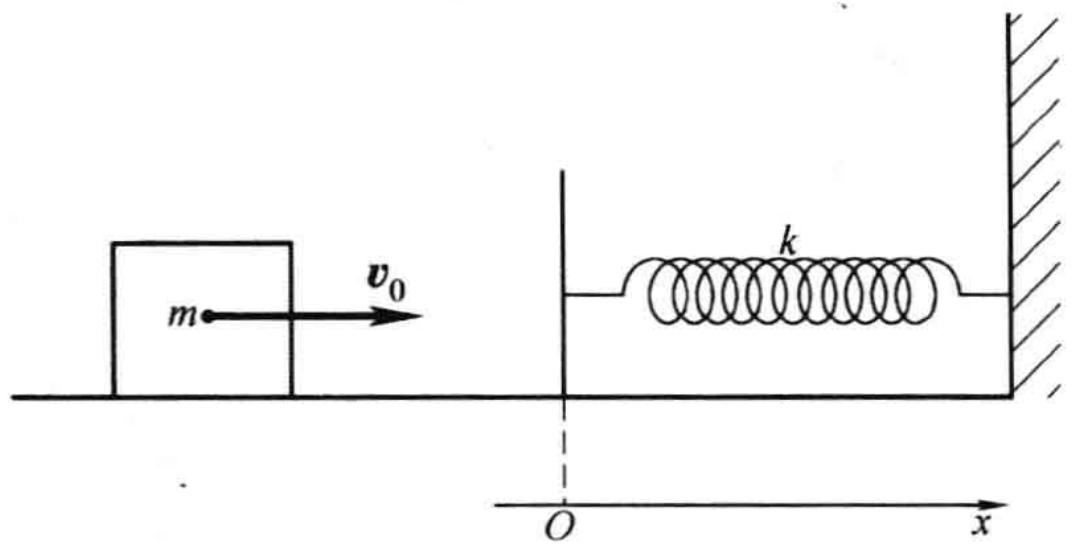
\includegraphics[width=0.35\textwidth]{figures/fig5-7.jpg}
  \end{figure}

\vfill

\textbf{5-8.}质量为 $m$ 的小球通过一根长为 $2l$ 的细绳悬挂于 $O$ 点。在 $O$ 点的正

下方 l 远处有一个固定的钉子 P。开始时，把绳拉至水平位置，然后释放小球。试求：当细绳碰到钉子后小球所能上升的最大高度。

\begin{figure}[H]
  \centering
  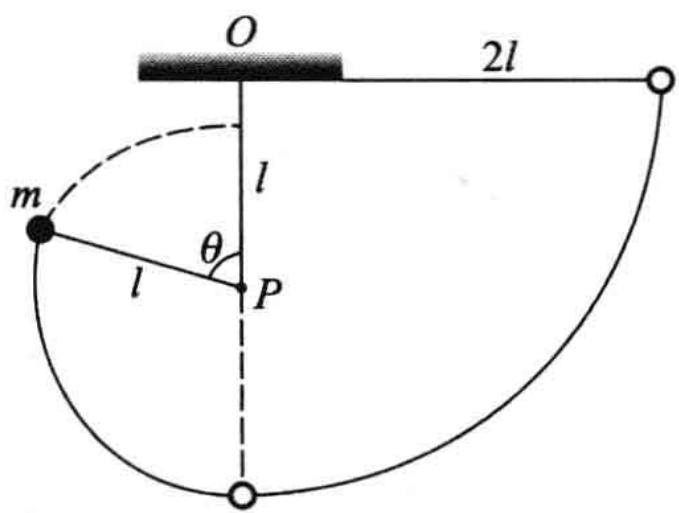
\includegraphics[width=0.25\textwidth]{figures/fig5-8.jpg}
  \end{figure}

\vfill
\newpage

\textbf{5-9.}如习题 5-9 图所示, 质量为 $m_{0}$ 的两质点分别固定在 $x$ 轴上的 $A(-a, 0)$ 、 $B(a,0)$ 两点, 若有一质点 $m$ 在万有引力作用下从 $y=3a$ 处由静止开始向原点运动。试求质点经过原点时的速度。

\begin{figure}[H]
  \centering
  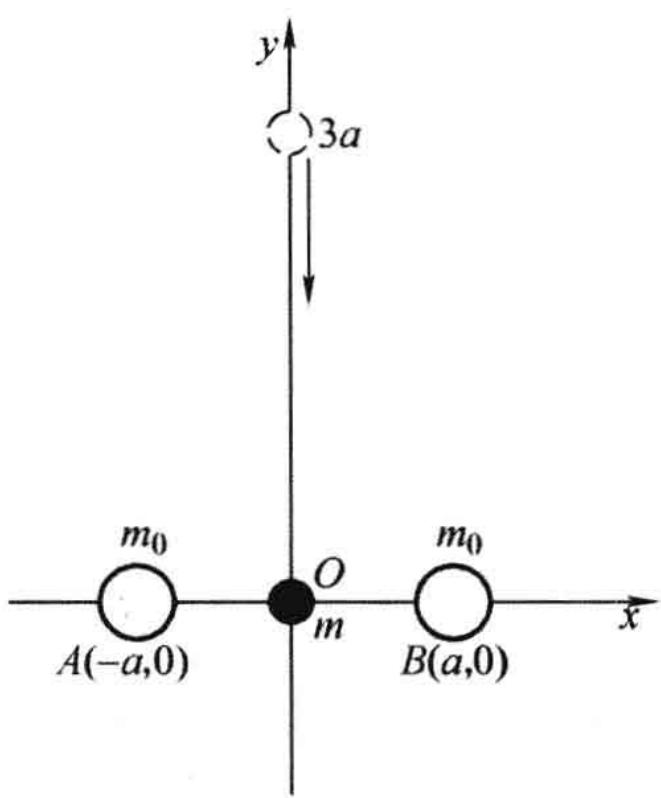
\includegraphics[width=0.25\textwidth]{figures/fig5-9_5.jpg}
  \end{figure}

\vfill

\textbf{5-10.}某人在地面上双脚起跳可使他的重心升高 $h$ 。现在他和另一个体重同为 $m_{1}$ 的人分别站在轻滑轮两边的秤盘中，如习题5-10图所示。盘重均为

$m_{2}$ 。试求:当此人在秤盘中用和在地面上起跳同样的能量双脚起跳时,他的重心可升高多少?

\begin{figure}[H]
  \centering
  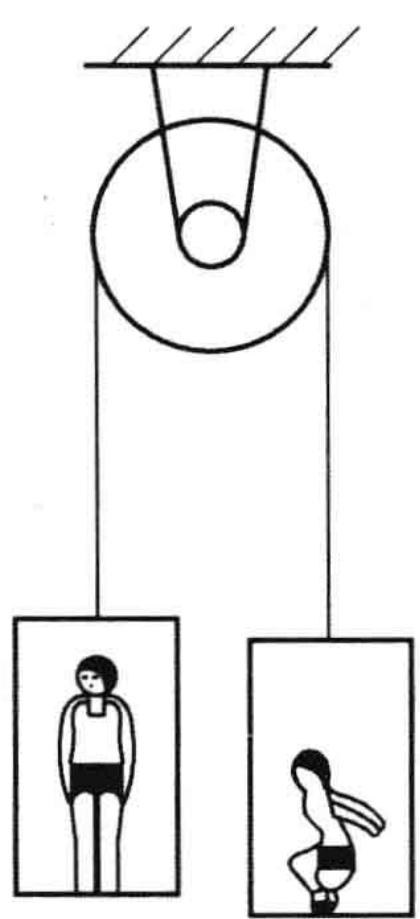
\includegraphics[width=0.13\textwidth]{figures/fig5-10.jpg}
  \end{figure}

\vfill
\newpage

\textbf{5-11.}在光滑半球形碗底静放着一质量 $m = 50 \mathrm{~g}$ 的光滑小球 B, 另一与 B 完全相同的小球 A 从高为 $h = 5.0 \mathrm{~cm}$ 的碗内壁处由静止滑下。若 A、B 球的碰撞为非弹性碰撞, 恢复系数为 $e = 0.6$ 。求 B 球被碰后能升多高?

\vfill

\textbf{5-12.}在光滑的水平桌面上有三个弹性小环 A、B、C, 它们的质量分别为 $m$ 、 $m 、 \alpha m (\alpha > 1)$ , 并依次排列在一条直线上。开始时, B、C 静止, 并挨在一起, 而 A 以 $v_{0}$ 的速度向 B 运动。试证明, 当它们之间的碰撞结束时, B 环静止, 而 A、C 的运动状态和没有 B 环时 A、C 碰撞后的运动状态一样。

\vfill
\newpage


\textbf{5-13.}一小球与两个相同的弹簧相连, 如习题 5-13 图所示。当小球平衡时, 两弹簧均受到拉伸。若忽略重力, 试讨论小球平衡的稳定性。

\begin{figure}[H]
  \centering
  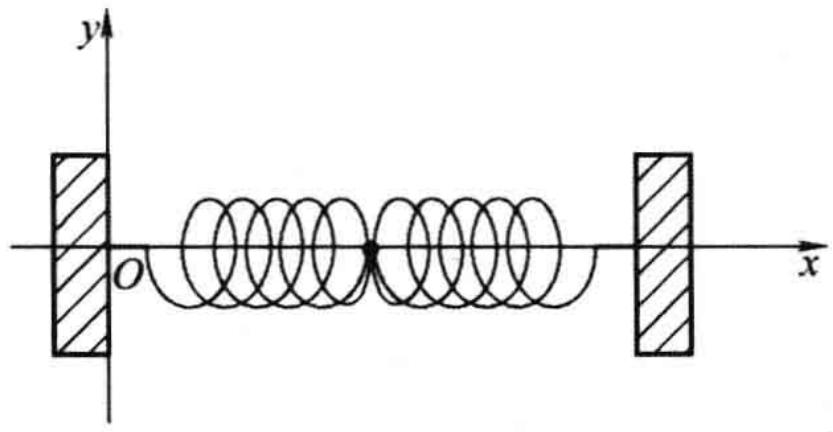
\includegraphics[width=0.35\textwidth]{figures/fig5-13.jpg}
  \end{figure}

\vfill

\textbf{5-14.}一质量为 $m$ 的质点在保守力的作用下沿 $x$ 轴（在 $x > 0$ 范围内）运动，其势能的数值为： $E_{\mathrm{p}} = \frac{A}{x^3} - \frac{B}{x}$ ，其中 $A, B$ 均为大于零的常量。

(1) 画出势能曲线图；

(2) 确定势阱的深度(最低点势能值);

（3）找出质点运动中受到沿 x 轴负方向最大力的位置；

(4) 若质点的总能量 E=0，试确定质点的运动范围。（本题中 x 以 m 为单位， $E_{p}$ 以 J 为单位。）

\begin{figure}[H]
  \centering
  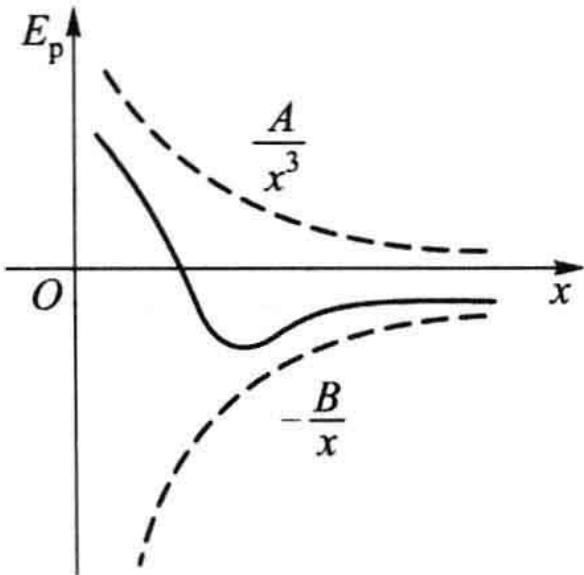
\includegraphics[width=0.25\textwidth]{figures/fig5-14_2.jpg}
  \end{figure}

\vfill
\newpage

\textbf{5-15.}一质量为 $m$ 的质点在保守力的作用下沿 $x$ 轴方向运动, 其势能的数值为: $E_{\mathrm{p}} = ax^{2}(b - x)(x$ 的单位是 $\mathrm{m}, E_{\mathrm{p}}$ 的单位是 $\mathrm{J}$ ), 其中 $a, b$ 均为大于零的常量。

(1) 试求质点所受力的表达式;

(2) 画出势能曲线图；

(3) 确定平衡位置,并讨论平衡位置的稳定性;

(4) 若质点从原点 $x = 0$ 处以 $v_{0}$ 开始运动, 试问, $v_{0}$ 在什么范围内质点不可能到达无穷远?

\begin{figure}[H]
  \centering
  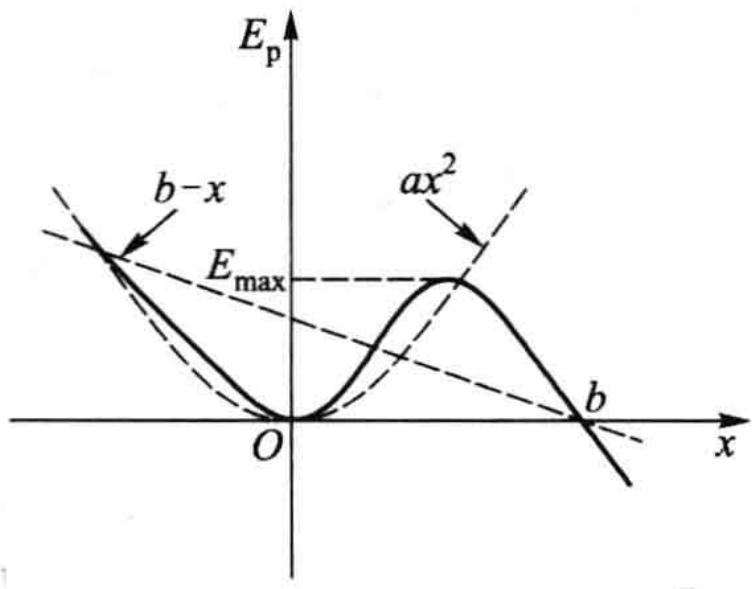
\includegraphics[width=0.3\textwidth]{figures/fig5-15.jpg}
  \end{figure}

\vfill

\textbf{5-16.}一颗质量为 $m$ 的人造地球卫星以圆形轨道环绕地球飞行。由于受到空气阻力的作用, 其轨道半径从 $r_1$ 变小到 $r_2$ 。求在此过程中空气阻力所做的功。

\vfill
\newpage

\textbf{5-17.}如习题 5-17 图所示, 物体从高为 $h$ 的斜面顶端自静止开始滑下, 最后停在与起点的水平距离为 $s$ 的水平地面上。若物体与斜面和与地面间的摩擦因数均为 $\mu$ , 证明 $\mu = h / s$ 。

\begin{figure}[H]
  \centering
  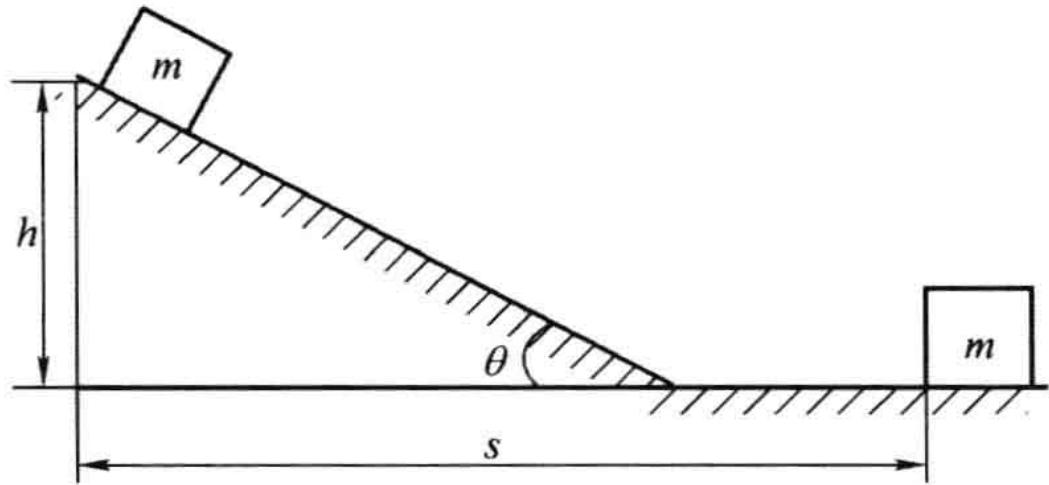
\includegraphics[width=0.35\textwidth]{figures/fig5-17.jpg}
  \end{figure}

\vfill

\textbf{5-18.}若上题中物体与斜面间摩擦因数和物体与地面之间的摩擦因数并不相同。当物体自斜面顶端静止滑下时, 停在地面上的 $A$ 点, 而当物体以 $v_{0}$ 的初速度 (方向沿斜面向下) 自同一点滑下时, 则停在地面上的 $B$ 点。已知 $A 、 B$ 点与斜面底端 $C$ 点的距离之间满足 $B C = 2 A C$ 。试求物体在斜面上运动的过程中摩擦力所做的功。

\vfill
\newpage

\textbf{5-19.}一光滑圆环, 半径为 $R$ , 用细线悬挂在支点上。环上穿有质量都是 $m$ 的两颗珠子, 让两珠子从环顶同时静止释放并向两边下滑。若圆环的质量为 $m_0$ , 试证明: 只有当 $m > \frac{3}{2} m_0$ 时, 圆环才会升起, 并求出珠子所在半径与细线所在竖直线的夹角 $\theta$ 。

\begin{figure}[H]
  \centering
  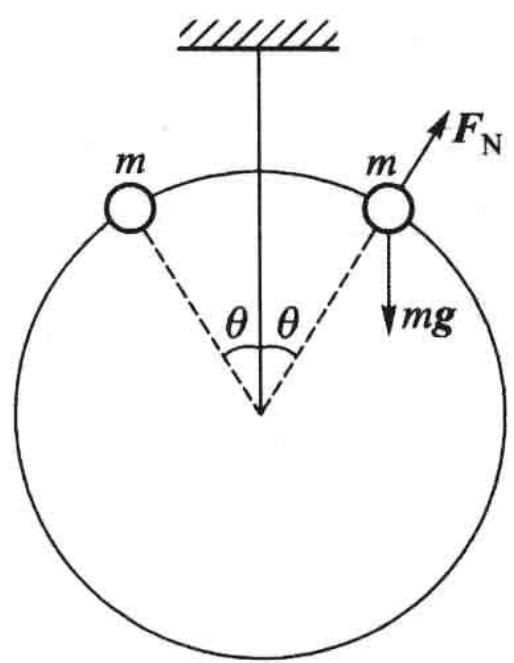
\includegraphics[width=0.23\textwidth]{figures/fig5-19.jpg}
  \end{figure}

\vfill

\textbf{5-20.}物体沿习题 5-20 图所示的光滑轨道自点 $A$ 由静止开始滑下。轨道的圆环部分有一对称的缺口 $BC$ , 缺口的张角 $\angle BOC = 2\alpha$ , 圆环的半径为 $R$ 。试问: A 点的高度 h 应等于多少才能使物体恰好越过缺口而走完整个圆环?

\begin{figure}[H]
  \centering
  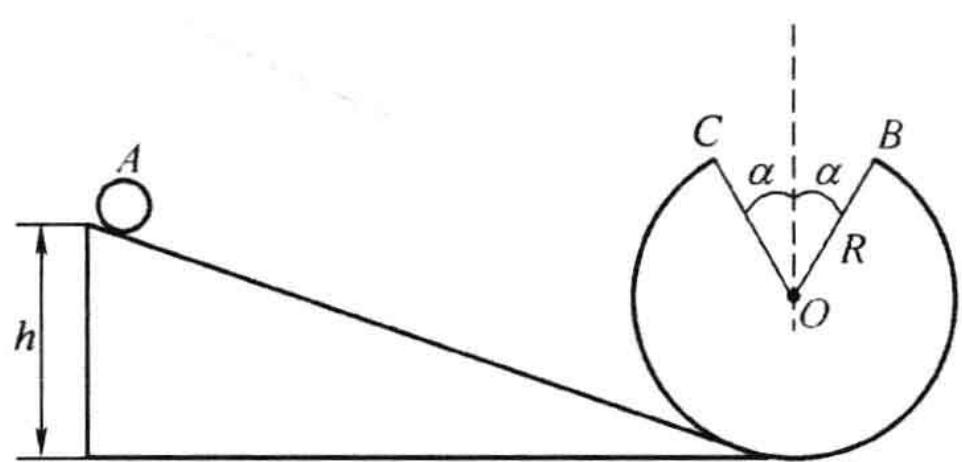
\includegraphics[width=0.35\textwidth]{figures/fig5-20.jpg}
  \end{figure}

\vfill
\newpage

\textbf{5-21.}如习题 5-21 图所示, 质量为 $m$ 的物体从光滑轨道的顶端 $A$ 点, 由静止开始沿斜道滑下, 在半径为 $R$ 的圆环部分的最低点 $B$ 与另一质量为 $m_0$ 的静止物体发生弹性碰撞, 碰后 $m_0$ 沿圆环上升, 并在高度为 $h_0$ 处脱离圆环, 而 $m$ 则沿斜道上升后又滑下, 并在 $m_0$ 脱离点脱离圆环。试求:

(1) m 与 $m_{0}$ 之比；

(2) A 点的高度 h。

\begin{figure}[H]
  \centering
  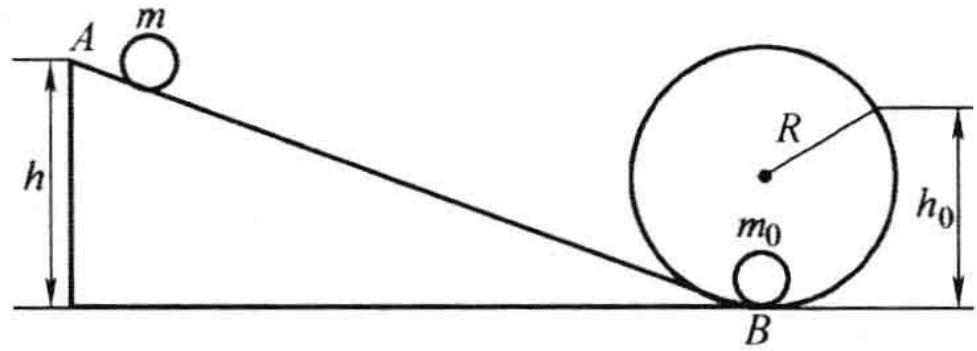
\includegraphics[width=0.32\textwidth]{figures/fig5-21.jpg}
  \end{figure}

\vfill

\textbf{5-22.}质量分别为 $m_{1}$ 和 $m_{2}$ 的两个物块由一劲度系数为 $k$ 的轻弹簧相连, 竖直地放在水平桌面上, 如习题 5-22 图所示。另有一质量为 $m$ 的物体从高出 $m_{1}$ 为 $h$ 的地方由静止开始自由落下, 当与 $m_{1}$ 发生碰撞后, 即与 $m_{1}$ 黏合在一起向下运动。试问 $h$ 至少应多大, 才能使得弹簧反弹后 $m_{2}$ 与桌面互相脱离?

\begin{figure}[H]
  \centering
  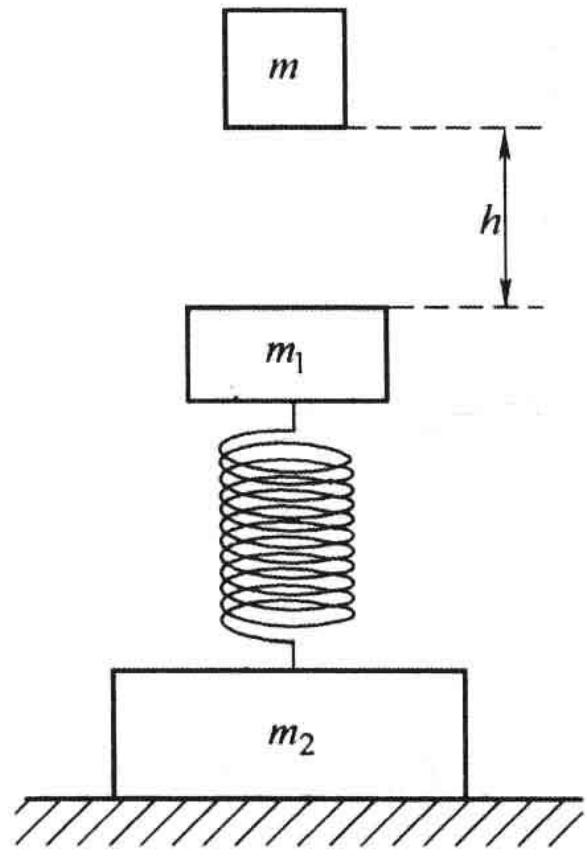
\includegraphics[width=0.2\textwidth]{figures/fig5-22.jpg}
  \end{figure}

\vfill
\newpage

\textbf{5-23.}在水平桌面上, 质量分别为 $m_{1}$ 和 $m_{2}$ 的两物块由一劲度系数为 $k$ 的弹簧相连。物块与桌面间的摩擦因数均为 $\mu$ 。开始时, 弹簧处于原长, $m_{2}$ 静止, 而 $m_{1}$ 以 $v_{0} = \sqrt{\frac{6m_{1}m_{2}g^{2}\mu^{2}}{k(m_{1} + m_{2})}}$ 的速度拉伸弹簧。试求: 当弹簧达最大拉伸时的伸长量 (设 $m_{1} > m_{2}$ ) 。

\vfill

\textbf{5-24.}质量分别为 $m_{1}$ 和 $m_{2}$ 的两物体发生非弹性正碰, 恢复系数为 $e$ 。试证明: 在质心坐标系中碰撞时损失的动能为其初始动能的 $(1 - e^{2})$ 倍。

\vfill
\newpage

\textbf{5-25.}长为 $2a$ 的轻绳两端各系有一质量为 $m$ 的小球, 中点处系有一质量为 $m_0$ 的小球, 三球排成一直线静置于光滑水平台面, 绳恰被拉直。对小球 $m_0$ 施以冲力, 使其获得与绳垂直的初速度 $v_0$ , 求:

(1) 当两小球 m 相碰的瞬时各球的速率;

(2) 当两小球 m 相碰的瞬时绳中的张力;

(3) 若从 $m_0$ 启动到两球 $m$ 相碰历时 $t$ , 而在此期间 $m_0$ 行进的距离为 $x$ , 试证明: $(m_0 + 2m)x = m_0v_0t + 2ma$ 。

\vfill

\textbf{5-26.}边长为 $a$ 的正方体木块静浮于横截面积为 $4a^{2}$ 的杯内水面上, 水的深

度 $h = 2a$ 。已知水的密度为 $\rho_0$ ，木块的密度为 $\frac{1}{2}\rho_0$ ，现将木块非常缓慢地压至水底。忽略水的阻力作用，求在此过程中外力所做的功。

\begin{figure}[H]
  \centering
  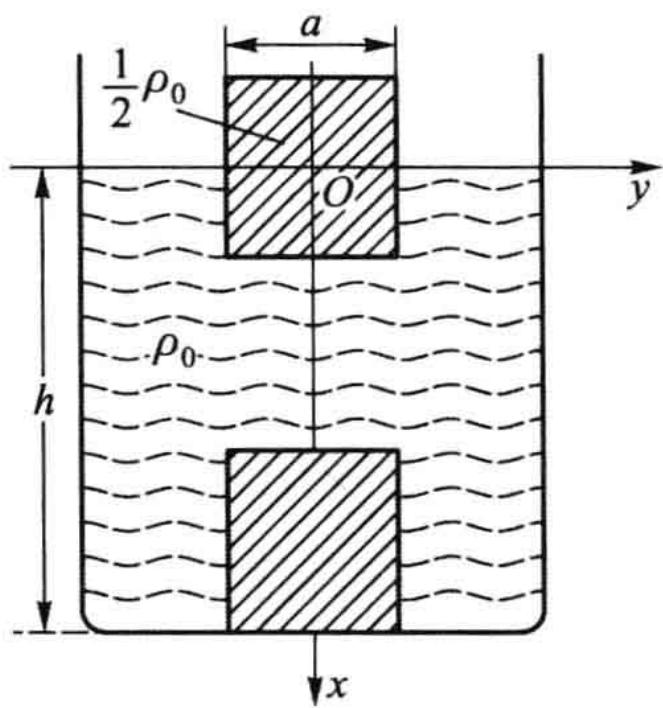
\includegraphics[width=0.25\textwidth]{figures/fig5-26.jpg}
  \end{figure}

\vfill
\newpage

\textbf{5-27.}一条长为 $2 l$ 、质量为 $m$ 的柔软绳索, 挂在一光滑的水平轴钉 (粗细可忽略) 上, 当两边的绳长均为 $l$ 时, 绳索处于平衡状态。若给其一端加一个竖直方向的微小扰动, 则绳索就从轴钉上滑落。试求:

(1) 当绳索刚脱离轴钉时, 绳索的速度;

(2) 当较长的一边绳索的长度为 x 时, 轴钉上所受的力。

\vfill

\textbf{5-28.}在竖直平面内有一光滑的半圆形管道, 圆的半径为 $R$ 。管内有一条

长度正好为半圆周长 $\pi R$ 的链条, 其线密度为 $\rho_{l}$ , 如习题 5-28 图所示。若由于微小的扰动, 链条从管口向外滑出。试求:

（1）当链条刚从管口全部滑出时的速度；

(2) 当链条从管口滑出的长度为 $\frac{\pi}{3} R$ 时的速度和加速度。

\begin{figure}[H]
  \centering
  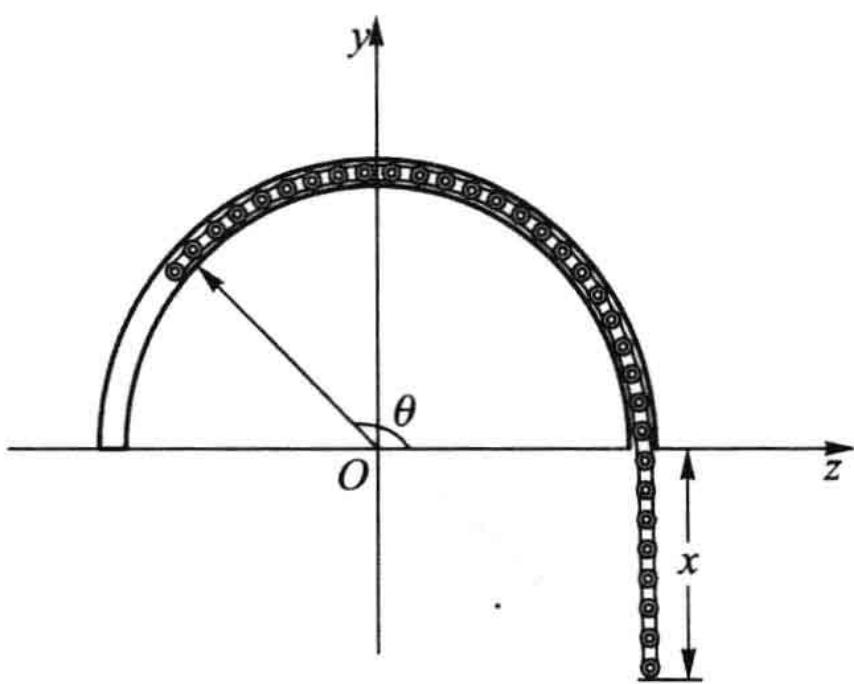
\includegraphics[width=0.33\textwidth]{figures/fig5-28.jpg}
  \end{figure}

\vfill
\newpage

\textbf{5-29.}在倾角 $\theta = \arctan \frac{3}{4}$ 的光滑斜面上叠放着质量 $m_{1} = 40 \mathrm{~kg}$ 的重物和质量 $m_{2} = 20 \mathrm{~kg}$ 、长 $l = 0.2 \mathrm{~m}$ 的板, 重物与板之间的摩擦因数 $\mu = 0.5$ 。 $m_{1}$ 与另一质量 $m = 30 \mathrm{~kg}$ 的重物由一跨过装在斜面顶端的定滑轮的细绳相连, 如习题 5-29 图所示。开始时, $m_{1}$ 和 $m_{2}$ 均静靠在斜面上一挡板处, $m$ 由手托住, 使绳松弛, 然后放手, 当 $m$ 自由下落的高度为 $h$ 时, 绳被拉紧。若 $m_{1}$ 体积很小, 以致可忽略其线度, 并设斜面和 $m$ 的运动长度足够长。忽略绳与滑轮的质量和滑轮轴承处的摩擦力。

（1）试分析由此三物体组成的系统以后运动的情况；

(2) 一种分析是, 若 $h$ 不太大时, 则 $m_{1}$ 和 $m_{2}$ 在以后的运动过程中不会互相脱离。这种分析是否正确? 如是正确的话, 求出 $h$ 的最大值。

\begin{figure}[H]
  \centering
  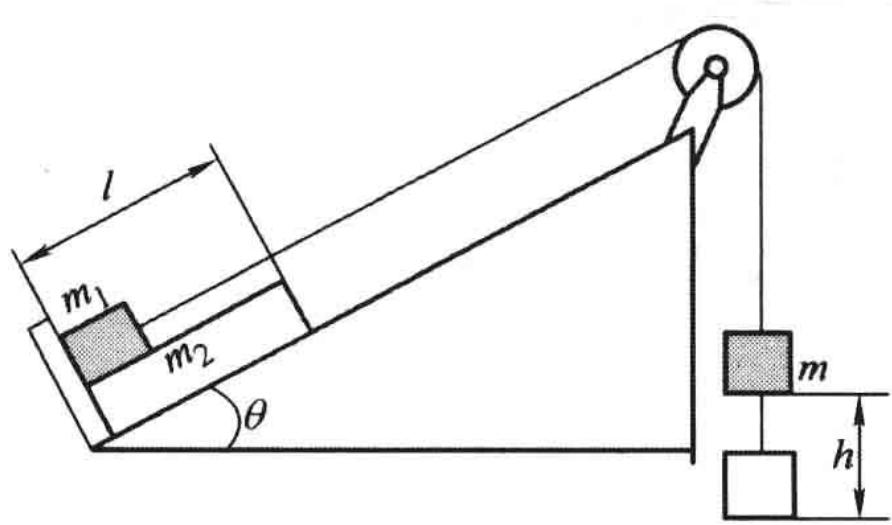
\includegraphics[width=0.3\textwidth]{figures/fig5-29.jpg}
  \end{figure}

\vfill

\textbf{5-30.}如习题 5-30 图所示,一个人手持质量为 $m$ 的小球乘坐在热气球下的吊篮里。气球、吊篮和人的总质量为 $m_0$ 。整个系统静止在空中。突然,人将小球向上急速抛出,经过时间 $t$ 后小球又返回人手中。若人手在抛接球时相对吊篮的位置不变,试求人在抛球过程中对系统做的功。

\begin{figure}[H]
  \centering
  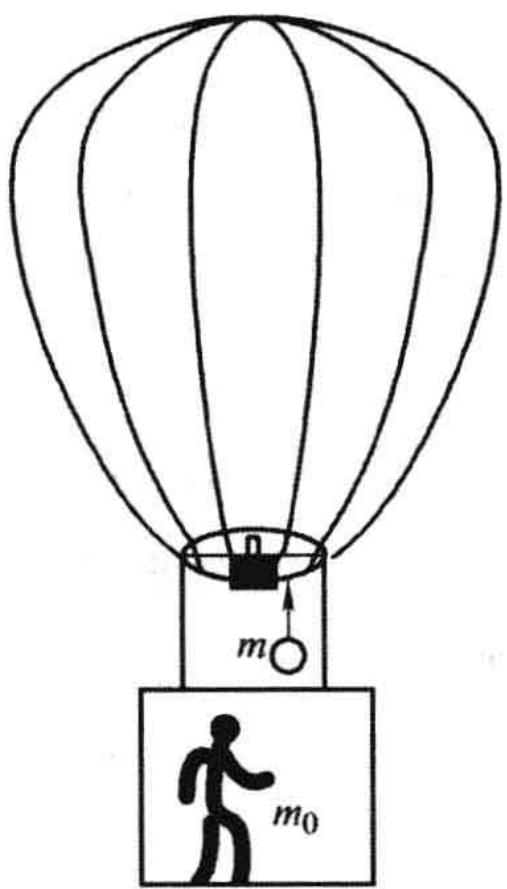
\includegraphics[width=0.2\textwidth]{figures/fig5-30.jpg}
  \end{figure}

\vfill
\newpage

\textbf{5-31.}在光滑的水平面上有两个质量分别为 $m_{1}$ 和 $m_{2} (m_{1} < m_{2})$ 的物块, $m_{2}$ 上连有一轻弹簧, 如习题 5-31 图所示。第一次, 具有动能 $E_{0}$ 的 $m_{1}$ 与静止的 $m_{2}$ 相碰; 第二次, 具有动能 $E_{0}$ 的 $m_{2}$ 与静止的 $m_{1}$ 相碰, 两次碰撞均压缩轻弹簧。试问:

(1) 两次碰撞中哪一次弹簧的最大压缩量较大?

(2) 若碰前两物块的总动能为 $E_{0}$ , 则 $E_{0}$ 如何分配, 才能使在两物块碰撞过程中弹簧的最大压缩量最大?

\begin{figure}[H]
  \centering
  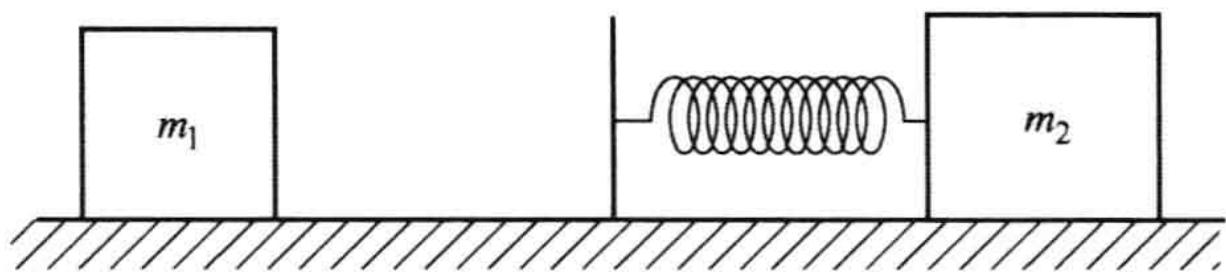
\includegraphics[width=0.35\textwidth]{figures/fig5-31_1.jpg}
  \end{figure}

\vfill

\textbf{5-32.}在光滑的水平面上, 一质量为 $m_{0}$ 的架子内连有一劲度系数为 $k$ 的弹簧,如习题5-32图所示。一质量为 $m$ 的小球以 $\pmb{u}$ 的速度射入静止的架子内,并开始压缩弹簧。设小球与架子内壁间无摩擦力。试求:

(1) 弹簧的最大压缩量；

(2) 从弹簧被压缩到弹簧达最大压缩量所需的时间；

(3) 在此过程中架子的位移。

\begin{figure}[H]
  \centering
  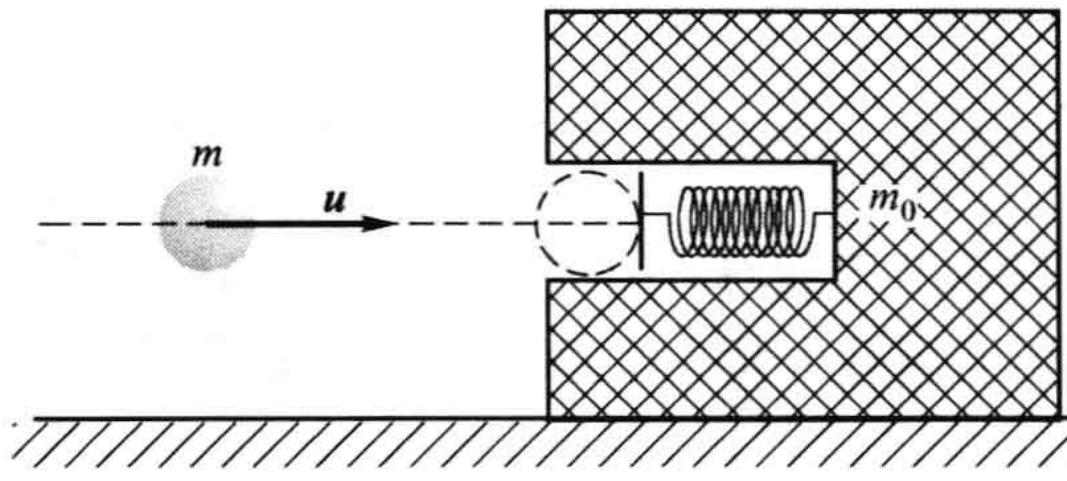
\includegraphics[width=0.33\textwidth]{figures/fig5-32.jpg}
  \end{figure}

\vfill
\newpage

\textbf{5-33.}在光滑的水平桌面上有三个完全相同光滑弹性小球, 两个静止小球 B、C 互相紧靠着, 另一小球 A 则以 $v_{0}$ 的速度沿 B、C 球心连线的中垂线向着两球运动。求碰后三球的速度。

\vfill

\textbf{5-34.}一运动粒子与另一质量与其相等的静止粒子发生弹性斜碰,试证

明:碰撞后两粒子的运动方向彼此垂直。

\begin{figure}[H]
  \centering
  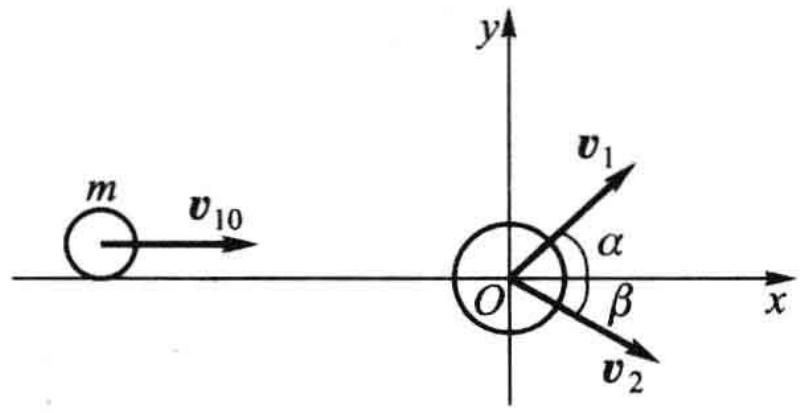
\includegraphics[width=0.4\textwidth]{figures/fig5-34.jpg}
  \end{figure}

\vfill
\newpage

\textbf{5-35.}一质量为 $2 \mathrm{~kg}$ 的小球 A 以 $v_{\mathrm{A} 0} = 32 \mathrm{~m} / \mathrm{s}$ 的速度与另一质量为 $6 \mathrm{~kg}$ 的静止小球 B 相碰。设碰撞是弹性的, 则在质心坐标系中, 两小球的反射角均为 $90^{\circ}$ 。试问:

(1) 在实验室坐标系中, A 球的反射角为多大?

(2) 在实验室坐标系中, 碰后 B 球的运动方向与 A 球原运动方向之间的夹角为多大?

\begin{figure}[H]
  \centering
  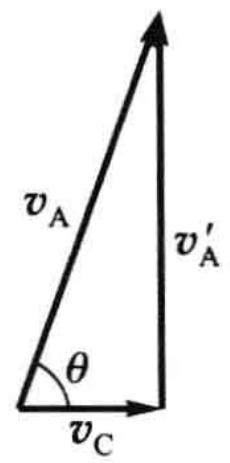
\includegraphics[width=0.1\textwidth]{figures/fig5-35_b.jpg}
  \end{figure}

\vfill

\textbf{5-36.}一质量为 $m$ 的质子以 $v_{0}$ 的速度去撞击静止质量为 $4 m$ 的氦核。在实验室坐标系里, 质子以 $\frac{1}{2} v_{0}$ 的速度和 $30^{\circ}$ 角散射。试求:

(1) 在实验室坐标系里, 撞击后氦核的速度及运动方向;

(2) 在质心坐标系里质子的散射速度, 以及两粒子的散射角度;

(3) 系统在散射中总能量的变化。

\vfill
\newpage


\textbf{6-1.}在给定的坐标系下, 设力 $F = 3i + 4k$ 的作用点位置矢量为: $\mathbf{r} = 2\mathbf{j} - 6\mathbf{k}$ , 其中 $\mathbf{F}$ 以 $\mathbf{N}$ 为单位, $\mathbf{r}$ 以 $\mathrm{m}$ 为单位, 求力对坐标原点的力矩。

\vfill

\textbf{6-2.}若将地球绕太阳的公转看作是以太阳为中心的圆周运动,试求地球相对太阳中心的角动量。已知地球的质量 $m_{\mathrm{E}} = 6.0 \times 10^{24} \mathrm{~kg}$ , 轨道半径 $R = 1.49 \times 10^{11} \mathrm{~m}$ 。

\vfill
\newpage

\textbf{6-3.}一质量 $m = 2 \mathrm{~kg}$ 的质点由静止开始做半径 $R = 5 \mathrm{~m}$ 的圆周运动。其相

对圆心的角动量随时间的变化关系为 $L=3t^{2}$ ，角动量 L 的单位为 $kg \cdot m^{2}/s, t$ 的单位为 s。

试求:(1) 质点受到的相对于圆心的力矩;

(2) 质点运动角速度随时间的变化关系。

\vfill

\textbf{6-4.}如习题 6-4 图所示, 一根轻绳跨过具有光滑水平轴的定滑轮(质量可忽略), 两个质量分别为 $m_{1}$ 和$m_{2}$ 的人各抓住绳子的一端。开始时，两人与水平轴之间的高度差分别为 $h_{1}$ 和 $h_{2}$ ，他们同时开始向上爬，并同时到达该滑轮的水平轴处。试求他们爬绳所经历的时间 t。

\begin{figure}[H]
  \centering
  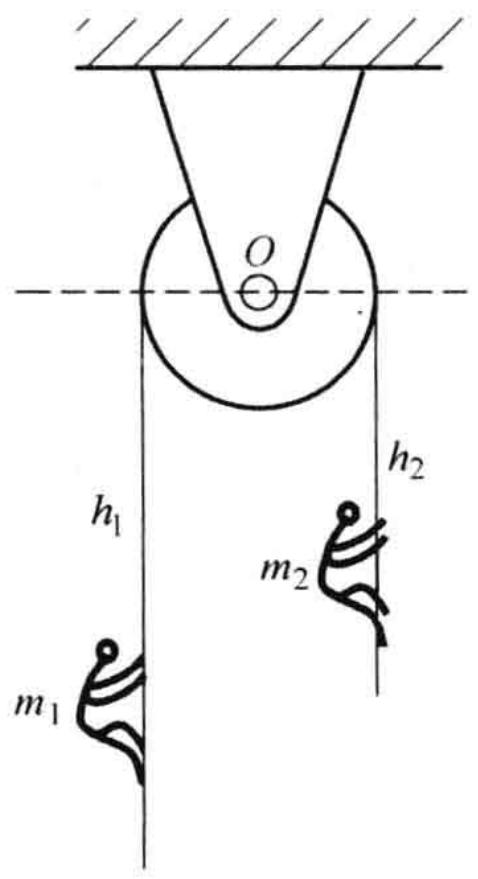
\includegraphics[width=0.2\textwidth]{figures/fig6-4.jpg}
  \end{figure}

\vfill
\newpage

\textbf{6-5.}在光滑的水平面上, 用长为 $l$ 的轻线连接两个质量分别为 $m_{1}$ 和 $m_{2}$ 的小球。开始时, 线正好拉直, $m_{1}$ 和 $m_{2}$ 的速度分别为 $v_{1}$ 和 $v_{2} (v_{1} > v_{2})$ , 它们的方向相同, 且垂直于连线。试问:

(1) 系统相对质心的角动量为多大?

(2) 线中的张力为多大?

\begin{figure}[H]
  \centering
  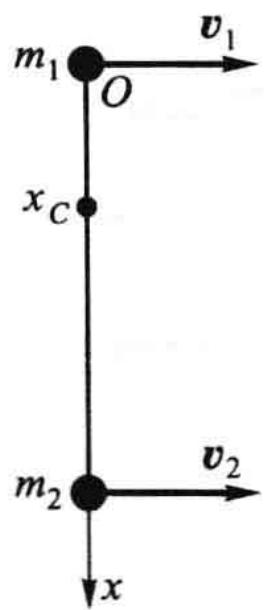
\includegraphics[width=0.1\textwidth]{figures/fig6-5.jpg}
  \end{figure}

\vfill

\textbf{6-6.}两个质量均为 $60 \mathrm{~kg}$ 的滑冰者, 在两条相距 $10 \mathrm{~m}$ 的平直跑道上以 $6.5 \mathrm{~m} / \mathrm{s}$ 的速率沿相反方向匀速滑行。当他们之间的距离恰好等于 $10 \mathrm{~m}$ 时, 他们分别抓住一根长 $10 \mathrm{~m}$ 的绳子的两端。若将滑冰者看成质点, 并略去绳子的质量。

(1) 求他们抓住绳子前后相对于绳子中点的角动量;

(2) 两人都用力缓慢往自己这边拉绳子, 当他们之间的距离为 $5 \mathrm{~m}$ 时, 各自的速率是多大?

(3) 求此时绳中的张力；

(4) 计算每个人在拉绳过程中所做的功。

\vfill
\newpage

\textbf{6-7.}一颗人造地球卫星沿椭圆轨道绕地球运行。在近地点, 卫星与地球中心的距离为地球半径的 3 倍。而在近地点, 卫星的速度为在远地点时的 4 倍。求在远地点时卫星与地球中心之间的距离为地球半径的多少倍。

\vfill

\textbf{6-8.}由火箭将一颗人造卫星送入离地面很近的轨道, 进入轨道时, 卫星的速度方向平行于地面, 其大小为在地面附近做圆周运动的速度的 $\sqrt{1.5}$ 倍。试求该卫星在运行中与地球中心的最远距离。

\vfill
\newpage

\textbf{6-9.}试求月球表面的重力加速度和从月球表面逃逸的速度。已知月球的半径 $R_{\text{月球}} = 1.7 \times 10^{6} \mathrm{~m}$ , 月球的质量 $m_{\text{月球}} = 7.3 \times 10^{22} \mathrm{~kg}$ 。

\vfill

\textbf{6-10.}在光滑水平桌面上, 质量分别为 $m_0$ 和 $m$ 的两物体系于原长为 $a$ , 劲度系数为 $k$ 的弹簧的两端。现使 $m_0$ 获得一与弹簧垂直的速度 $v_0$ 。试证明: 若 $v_0 = 3a \sqrt{\frac{k}{2m'}}$ , 其中 $m'$ 为约化质量, 则在以后的运动过程中两物体之间的最大距离为 $3a$ 。

\vfill
\newpage


\textbf{6-11.}发射一宇宙飞船去考察一质量为 $m_{0}$ 、半径为 $R$ 的行星。当飞船静止于空间离行星中心 $5 R$ 处时, 以速度 $v_{0}$ 发射一包仪器, 如习题 6-11 图所示。仪器包的质量 $m$ 远小于飞船的质量, 要使该仪器包恰好掠擦行星表面着陆, $\theta$ 角应是多少?

\begin{figure}[H]
  \centering
  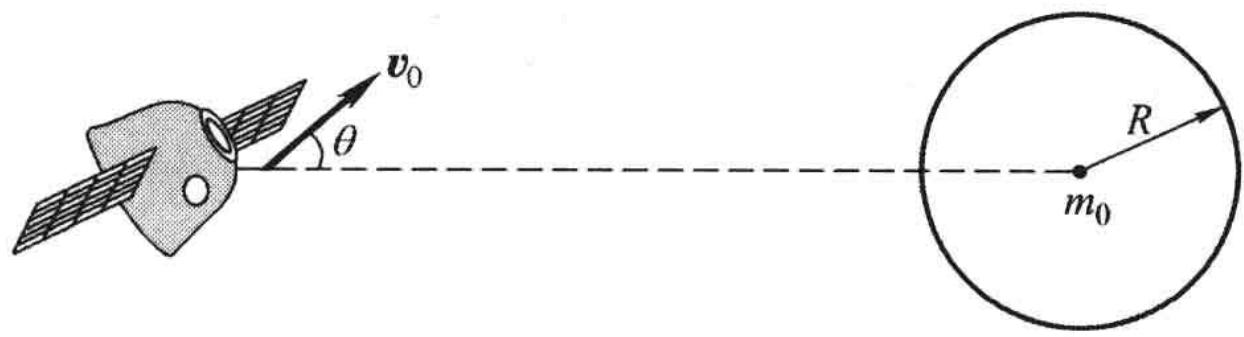
\includegraphics[width=0.4\textwidth]{figures/fig6-11_6.jpg}
  \end{figure}

\vfill

\textbf{6-12.}一质量为 $m$ 的空间站沿半径为 $r$ 的圆周绕月球运动。为使空间站能

在月球上登陆,当空间站运行至轨道上 P 点时向前发射一质量为 $m_{1}$ 的物体,来改变空间站的运行速度,从而使其沿习题 6-12 图所示的新轨道运动,并在月球表面登陆。已知月球的半径为 $R_{月}$ ,月球的质量为 $m_{月}$ ,试求 $m_{1}$ 的发射速度 $v_{1}$ (相对月球参考系)。

\begin{figure}[H]
  \centering
  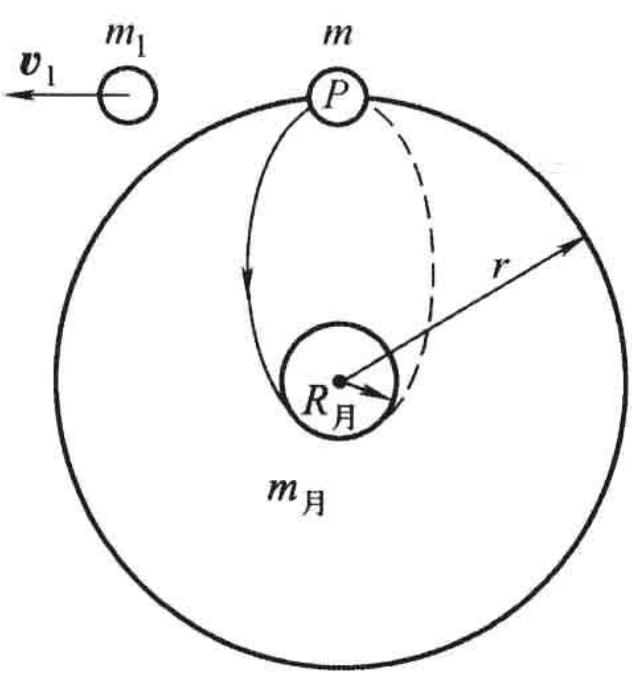
\includegraphics[width=0.23\textwidth]{figures/fig6-12.jpg}
  \end{figure}

\vfill
\newpage

\textbf{6-13.}质量为 $m$ 的质点在质量为 $m_0$ 的质点（视为固定）的引力场中以 $m_0$ 为中心做半径为 $r_0$ 的周期运动。若给 $m$ 以沿径向的冲量 $I$ , 并设 $I$ 与质点的原动量之比为一小量, 求 $m$ 在以后运动过程中径矢的最大值 $r_2$ 与最小值 $r_1$ , 并证明在忽略二级以上小量的情况下, $r_2 - r_0 \approx r_0 - r_1$ , 即质点 $m$ 的运动轨道近似为一偏心的圆。

\vfill

\textbf{6-14.}天狼星是天空中最明亮的恒星,因此人们很早就已开始观察它的运动。1844年德国天文学家弗里德里希·贝塞尔注意到天狼星运动的异常情况,并据此预言它附近有伴星。1862年美国阿尔文·克拉克首次观测到这一伴星(系白矮星,肉眼看不到)。根据以后的观测资料,该双星系统的运动轨迹如习题6-14图所示。图中粗、细实线分别表示天狼星与其伴星的运动轨迹,虚线为质心的运动轨迹,第一组黑点表示1862年的双星位置,其余各组黑点分别表示自1870年起至1940年每隔10年的双星位置。天狼星和伴星的平均距离为

s=20.4 AU(1 AU=1.496×10 $^{8}$ km)，它们与质心的距离之比约为2:5。

(1) 由图判断双星在相对做圆周运动还是椭圆运动? 运动周期是多少年?

(2) 假定双星相对做距离为 $a$ 的匀速圆周运动, 试估算天狼星及其伴星的质量 $m_{\mathrm{A}}$ 和 $m_{\mathrm{B}}$ (用太阳质量 $m_{\mathrm{S}}$ 表示)。

\begin{figure}[H]
  \centering
  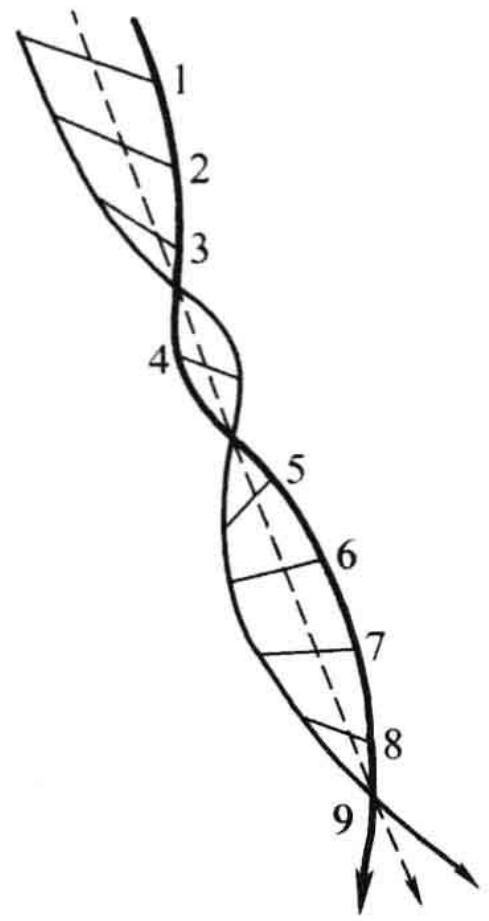
\includegraphics[width=0.18\textwidth]{figures/fig6-14.jpg}
  \end{figure}

\vfill
\newpage

\textbf{6-15.}如习题 6-15 图所示, 质量均为 $m$ 的小球 1、2 用长为 $4a$ 的细线相连, 以速度 $v$ 沿着与线垂直的方向在光滑水平台面上运动, 线处于伸直状态。在运动过程中, 线上距离小球 1 为 $a$ 的一点与固定在台面上的一竖直光滑细钉相碰, 设在以后的运动过程中两球不相碰。求:

(1) 小球 1 与钉的最大距离；

(2) 线中的最小张力。

\begin{figure}[H]
  \centering
  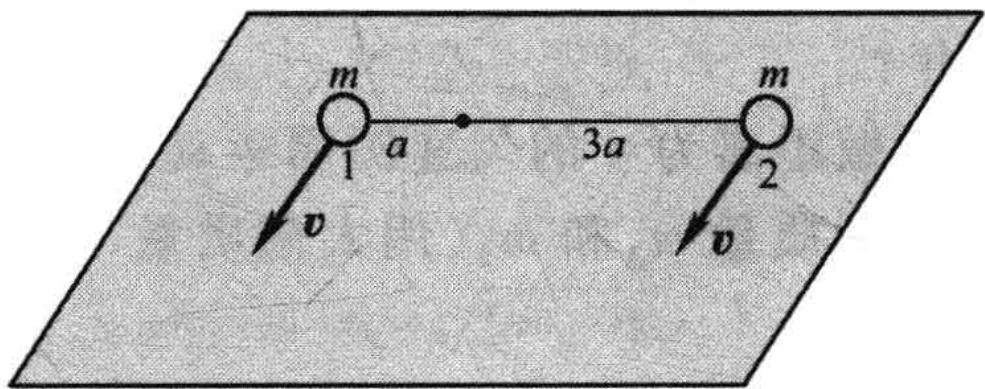
\includegraphics[width=0.28\textwidth]{figures/fig6-15.jpg}
  \end{figure}

\vfill

\textbf{6-16.}在一半径为 $R = 2.0 \times 10^{8} \mathrm{~m}$ 的无空气的星球表面, 若以 $v_{0} = 10 \mathrm{~m} / \mathrm{s}$ 的速度竖直上抛一物体, 则该物体上升的最大高度为 $h = 8 \mathrm{~m}$ 。试问:

(1) 该星球的逃逸速度有多大?

(2) 若要使该星球成为黑洞,则现有的半径应比黑洞的半径大几倍?

(本题可参考第十二章 12.3.5 节有关黑洞的介绍)

\vfill
\newpage


% Part 3
\textbf{7-1.}一根长为 $l$ 的不均匀细杆, 其线密度 $\lambda = a + bx$ ( $x$ 为离杆的一端 $O$ 的距离。 $a, b$ 为已知常量)。求该杆对过 $O$ 端并垂直于杆的轴的转动惯量。

\vfill

\textbf{7-2.}一质量为 $m_0$ 、半径为 $R$ 的均质圆盘, 可绕过其圆心且垂直于圆盘的光滑水平轴在竖直平面内转动。在盘的边上绕有一不可伸长的细绳, 绳的一端连有一质量为 $m$ 的物体。开始时, 绳子被拉直, 物体 $m$ 的高度为 $h$ , 并由静止开始

下降,设绳与盘边之间无相对滑动。试求:

(1) 绳的张力 $F_{T}$ ;

(2) 物体 m 到达地面所需的时间 t。

\begin{figure}[H]
  \centering
  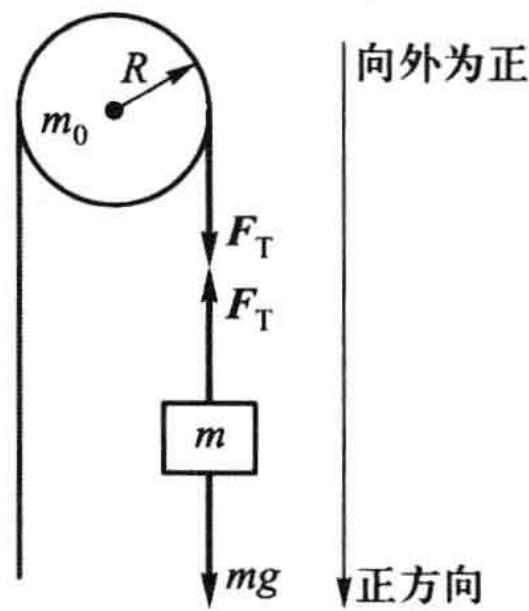
\includegraphics[width=0.25\textwidth]{figures/fig7-2.jpg}
  \end{figure}

\vfill
\newpage

\textbf{7-3.}在粗糙的水平面上,一半径为 $R$ 、质量为 $m$ 的均质圆盘绕过其中心且与盘面垂直的竖直轴转动,如习题 7-3 图所示。已知圆盘的初角速度为 $\omega_0$ ,圆盘与水平面间的摩擦因数为 $\mu$ ,若忽略圆盘轴承处的摩擦,问经过多长时间圆盘将静止?

\begin{figure}[H]
  \centering
  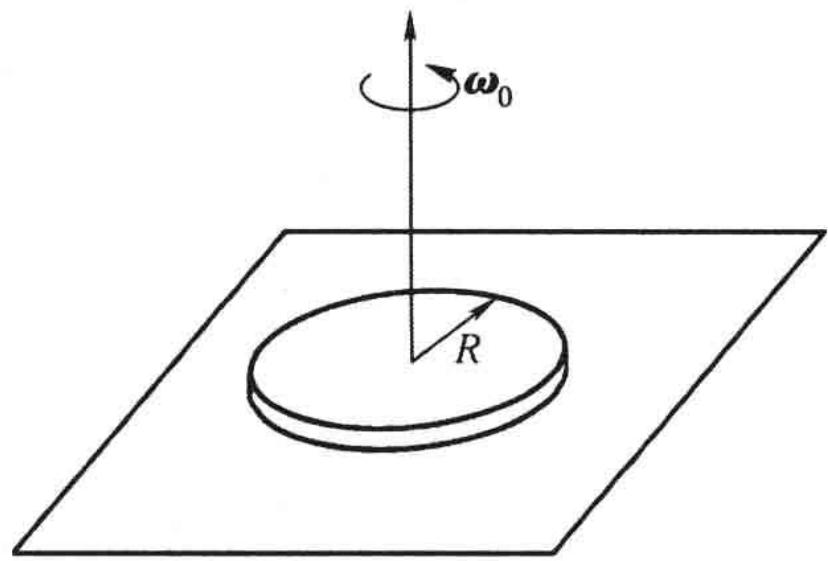
\includegraphics[width=0.3\textwidth]{figures/fig7-3.jpg}
  \end{figure}

\vfill

\textbf{7-4.}一个高为 $h$ 、底半径为 $R$ 的圆锥体, 可绕其固定的竖直轴自由旋转。在其表面沿母线刻有一条光滑的斜槽, 如习题 7-4 图所示。开始时, 锥体以角速度 $\omega_0$ 旋转, 此时, 将质量为 $m$ 的小滑块从槽顶无初速释放。设在滑块沿槽滑下的过程中始终不脱离斜槽，而锥体绕竖直轴的转动惯量为 $J_{0}$ 。试问：

(1) 当滑块到达底边时, 圆锥体的角速度为多大?

(2) 当滑块到达底边时, 滑块相对地面的速度为多大?

\begin{figure}[H]
  \centering
  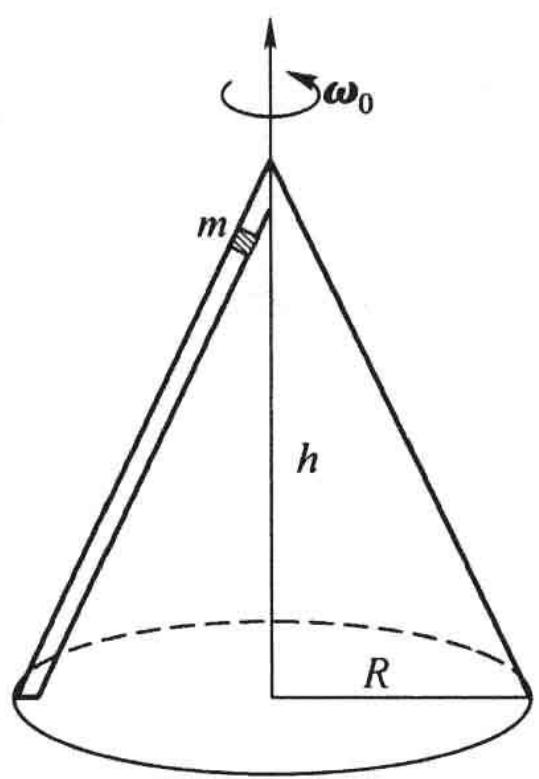
\includegraphics[width=0.2\textwidth]{figures/fig7-4_1.jpg}
  \end{figure}

\vfill
\newpage

\textbf{7-5.}质量为 $m$ 、半径为 $r$ 的均质球置于粗糙的水平面上, 球与水平面之间的摩擦因数为 $\mu$ 。开始时, 球的转动角速度为 $\omega_0$ 而质心静止。试问:

(1) 经过多长时间球开始做纯滚动?

(2) 球做纯滚动时质心的速度为多大?

\vfill

\textbf{7-6.}将一根长为 $L$ 、质量为 $m$ 的均匀杆上长为 $l\left(l < \frac{1}{2} L\right)$ 的一段搁在桌边，另一端用手托住，使杆处于水平状态，如习题 7-6 图所示。现释放手托的一端，试问，当杆转过的角度 $\theta$ 为多大时，杆开始滑离桌边（设杆与桌边之间的摩擦因数为 $\mu$ ）？

\begin{figure}[H]
  \centering
  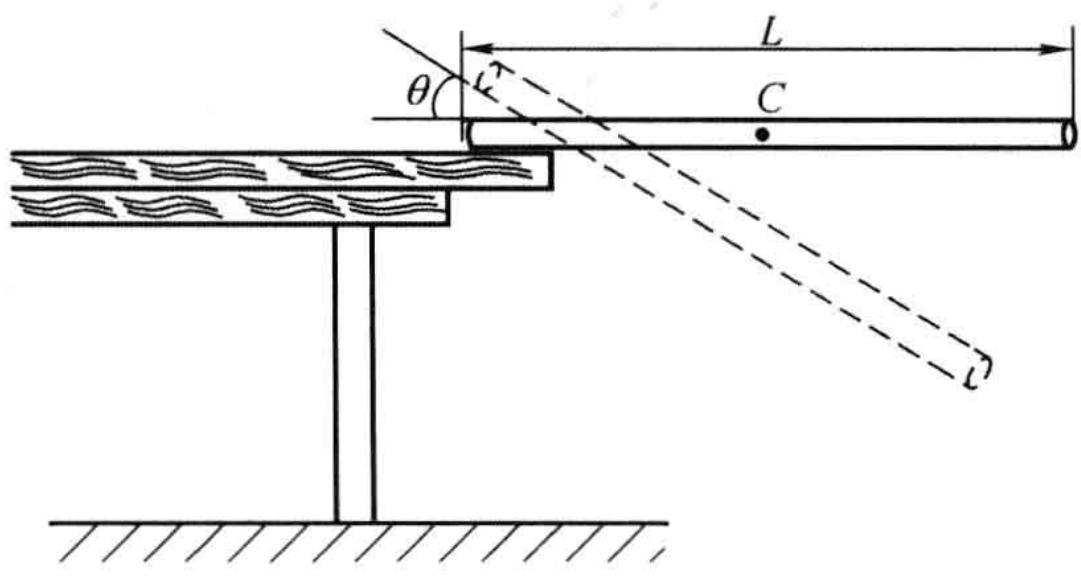
\includegraphics[width=0.4\textwidth]{figures/fig7-6.jpg}
  \end{figure}

\vfill
\newpage

\textbf{7-7.}质量为 $m$ 的子弹, 以速度 $v_{0}$ 射入质量为 $m_{0}$ 、半径为 $R$ 的圆盘的边缘, 并留在该处。 $v_{0}$ 的方向与入射处的半径垂直, 如习题 7-7 图所示。试就以下两种情况:

(1) 盘心装有一与盘面垂直的光滑固定轴;

(2) 圆盘是自由的。

求子弹射入后圆盘系统总动能之比 $E_{k1}/E_{k2}$ 。

\begin{figure}[H]
  \centering
  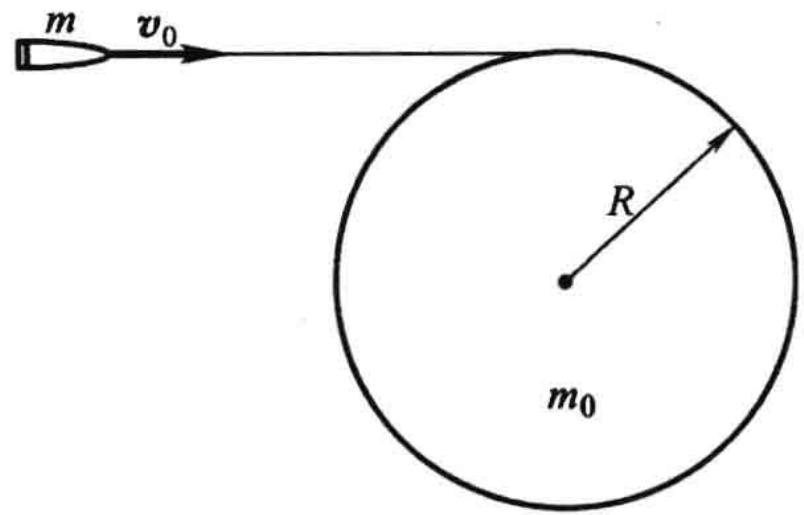
\includegraphics[width=0.3\textwidth]{figures/fig7-7_1.jpg}
  \end{figure}

\vfill

\textbf{7-8.}如习题 7-8 图所示, 质量为 $m_{0}$ 、半径为 $R$ 的弹性球在水平面上做纯滚

动,球心速度为 $v_{0}$ ,与粗糙的墙面发生碰撞后,以相同的球心速度反弹,设球与墙面、水平面的摩擦因数都为 $\mu$ , 碰撞时球与水平面的摩擦可以忽略。

（1）碰撞后，球经过一段时间开始做纯滚动，求此时的球心速度；

(2) 若球与墙面之间的碰撞时间为 $\Delta t$ , 为使碰撞时球不会跳起, 则摩擦因数应满足什么关系? 设碰撞过程中的相互作用力为恒力。

\begin{figure}[H]
  \centering
  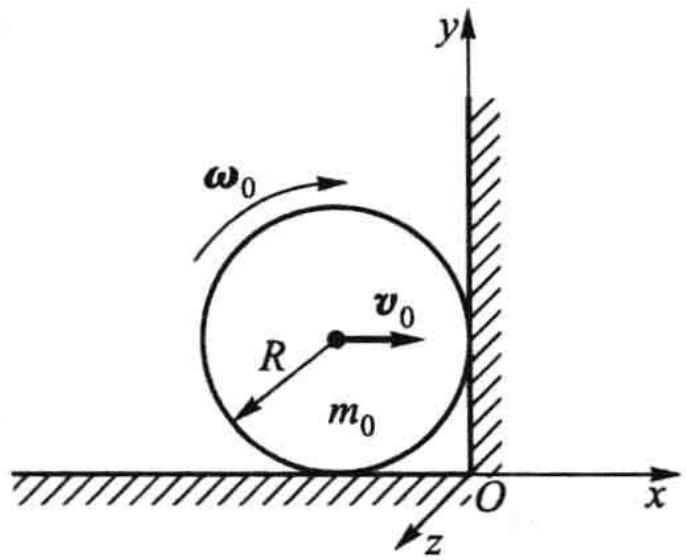
\includegraphics[width=0.33\textwidth]{figures/fig7-8.jpg}
  \end{figure}

\vfill
\newpage

\textbf{7-9.}一根长为 $2l$ , 质量为 $2m_0$ 的均匀细杆, 可以绕过中点的固定轴在水平面内自由转动。在离中心 $\frac{1}{3} l$ 处各套有两个质量均为 $m$ 的小珠子, 开始时杆的转动角速度为 $\omega_0$ , 而两小珠相对静止。当释放小珠后, 小珠将沿杆无摩擦地向两端滑动。试问:

(1) 当小珠滑至杆端时,杆的角速度为多大?

(2) 当小珠滑至杆端时, 小珠相对杆的速度为多大?

(3) 当小珠滑离杆时, 小珠的速度为多大?

\vfill

\textbf{7-10.}两根质量均为 $m$ 、长度均为 $l$ 的相同均质细杆 $AC$ 与 $CB$ , 两杆的 $C$ 端用一光滑的铰链相连。将两杆分开一定角度, 让 $A$ 、 $B$ 端与光滑地面接触, 并使两杆均在竖直平面内。开始时, 两杆与地面间的夹角均为 $\theta$ 。现无初速地释放两杆, 问两杆着地时 $C$ 点的速度。

\vfill
\newpage

\textbf{7-11.}两光滑墙面互相垂直, 在墙 B 上离墙面 A 距离 s 处, 有一光滑钉子,

将一长度为 2l、质量为 $m_{0}$ 的均匀杆的一端抵在墙上，杆身斜置在钉子上，使杆位于垂直于墙面 A 的竖直平面内，求平衡时杆与水平面所成的角 $\theta$ 。

\begin{figure}[H]
  \centering
  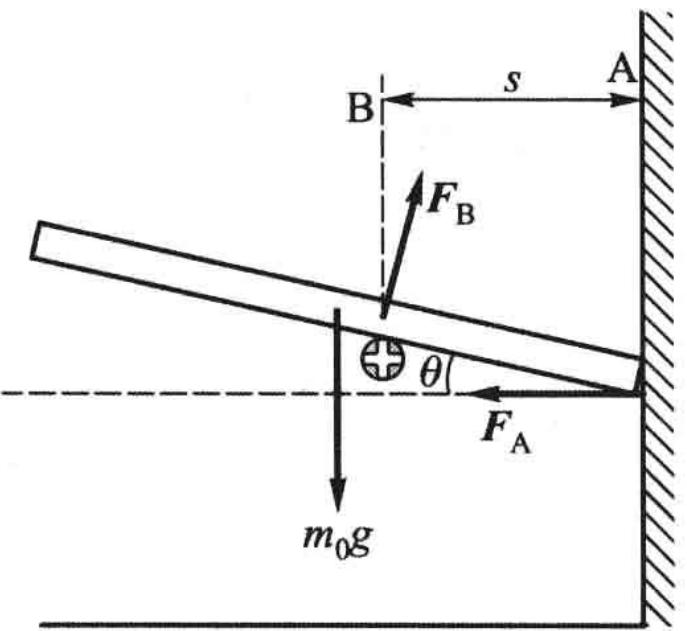
\includegraphics[width=0.25\textwidth]{figures/fig7-11.jpg}
  \end{figure}

\vfill

\textbf{7-12.}如习题 7-12 图所示, 一飞轮以 $\omega$ 的角速度高速转动, 其转动惯量为 $J_{0}$ , 试问, 为使水平圆台以恒定角速度 $\Omega$ 转动 ( $\Omega \ll \omega$ ), 则所需加在圆台上的力矩为多大?

\begin{figure}[H]
  \centering
  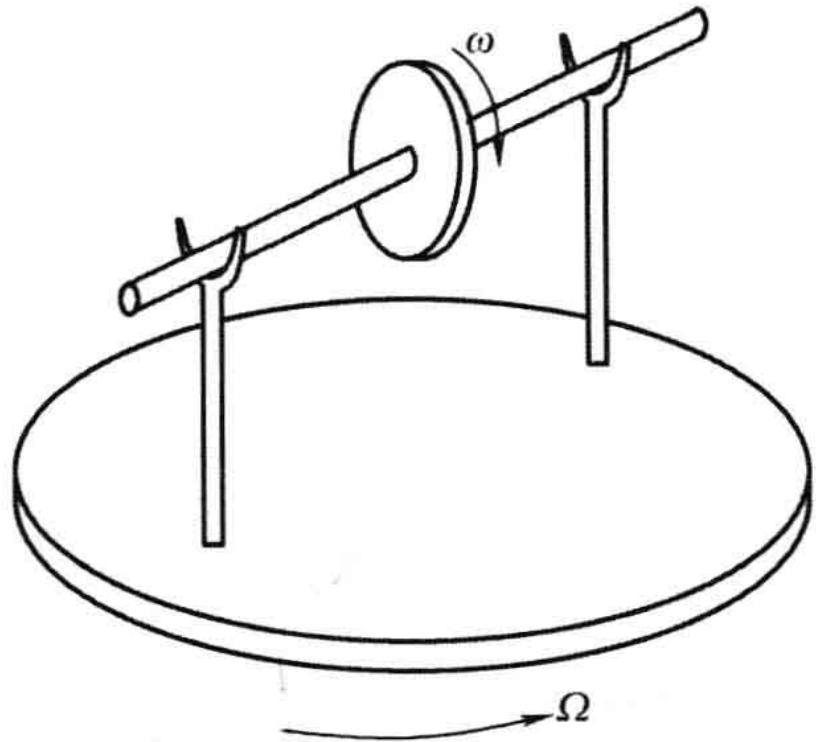
\includegraphics[width=0.25\textwidth]{figures/fig7-12.jpg}
  \end{figure}

\vfill
\newpage

\textbf{7-13.}在光滑水平面上, 质量均为 $m_{0}$ 的两小球由一长为 $l$ 的轻杆相连。另一质量为 $m$ 的小球以 $v_{0}$ 的速率向着与杆成 $\theta$ 角的方向运动, 并与某一 $m_{0}$ 发生碰撞, 碰后 $m$ 以 $\frac{1}{2} v_{0}$ 的速率沿原路线反弹。试求碰撞后轻杆系统绕其质心转动的角速度 $\omega$ , 参见习题 7-14 图。

\vfill

\textbf{7-14.}若上题中三球的质量相同, 均为 $m$ , 且 $\theta = 45^{\circ}$ 。当运动小球以 $v_{0}$ 的速率与连在杆上的某一球发生弹性碰撞后, 即沿垂直于原速度的方向运动, 如习题 7-14 图所示。试求:

(1) 碰撞后, 运动小球的速度 $v_{f}$ ;

(2) 碰撞后, 轻杆系统绕其质心转动的角速度 $\omega$ 。

\begin{figure}[H]
  \centering
  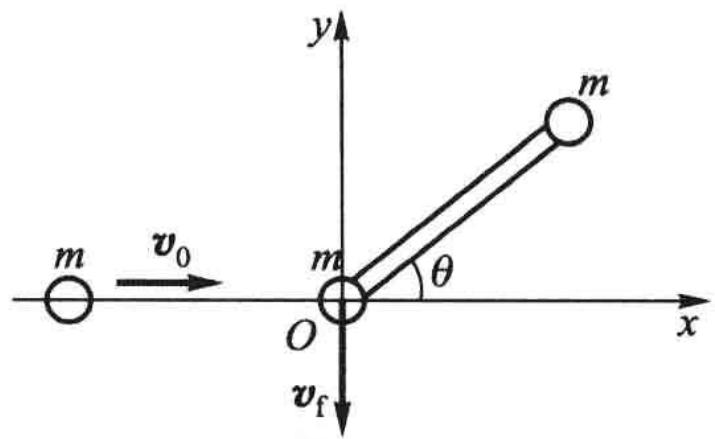
\includegraphics[width=0.4\textwidth]{figures/fig7-14.jpg}
  \end{figure}

\vfill
\newpage

\textbf{7-15.}一块边长为 $a$ 、质量为 $m_{0}$ 的正三角形薄板, 求该板对过其一边的轴的转动惯量。

\begin{figure}[H]
  \centering
  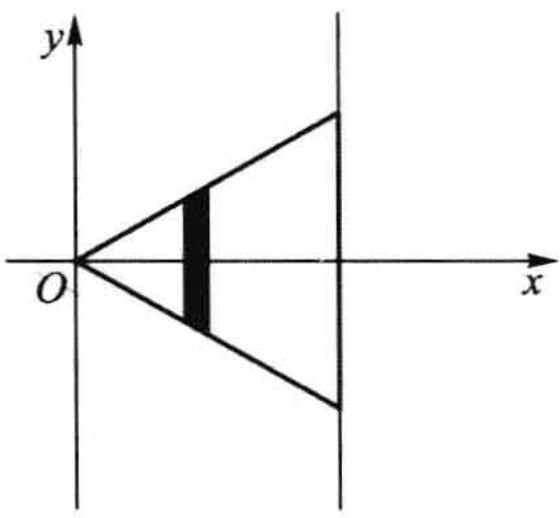
\includegraphics[width=0.3\textwidth]{figures/fig7-15.jpg}
  \end{figure}

\vfill

\textbf{7-16.}在质量为 $m_{0}$ 、半径为 $R$ 的匀质圆盘上, 有三个半径为 $\frac{1}{3} R$ 的小圆孔, 圆孔的圆心分别在三条半径的中心处, 此三条半径把圆盘分割成相等的三块, 如习题 7- 16 图所示。求此圆盘对过其圆心且与盘面垂直的轴的转动惯量。

\vfill
\newpage

\textbf{7-17.}两块质量均为 $m_{0}$ 、半径均为 $R$ 的均匀薄圆盘间连有一均匀细杆, 细杆长为 $l$ , 质量为 $m$ , 过两盘的圆心且与圆盘垂直, 如习题 7-17 图所示。求此装置对通过某一圆盘直径的轴的转动惯量。

\begin{figure}[H]
  \centering
  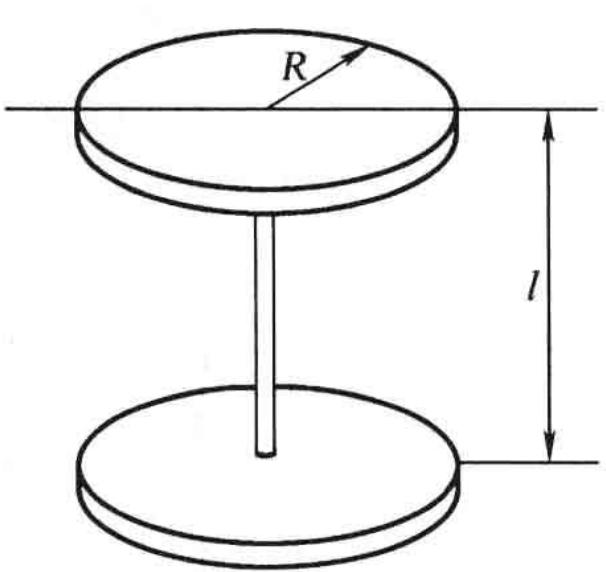
\includegraphics[width=0.25\textwidth]{figures/fig7-17.jpg}
  \end{figure}

\vfill

\textbf{7-18.}质量分别为 $m_{1} = 200 \mathrm{~g}, m_{2} = 250 \mathrm{~g}$ 的两个物体用细绳相连, 绳子套在质量 $m_{0} = 100 \mathrm{~g}$ , 半径 $r = 10 \mathrm{~cm}$ 的滑轮上, $m_{2}$ 放在光滑的水平桌面上, $m_{1}$ 悬挂着, 如习题 7-18 图所示。设滑轮为一质量均匀的圆盘, 绳子的长度不变, 绳子的质量及滑轮轴承处的摩擦均可忽略不计, 绳子与滑轮之间无滑动。求 $m_{1}$ 的加速度 $a$ 以及绳子各处的张力 $F_{\mathrm{T} 1}$ 和 $F_{\mathrm{T} 2}$ 。

\vfill
\newpage

\textbf{7-19.}如习题 7-19 图所示的阿特伍德机中, 两物体质量分别是 $m_{1}$ 和 $m_{2}$ ,

滑轮半径为 R，质量为 $m_{0}$ 。若物体运动时，滑轮与绳之间有相对滑动，两者之间的摩擦因数为 $\mu$ 。设绳不可伸长，忽略滑轮轴承处的摩擦。试求：

(1) $m_{1}$ 与 $m_{2}$ 的加速度；

(2) 滑轮的角加速度 $\alpha$ 。

\begin{figure}[H]
  \centering
  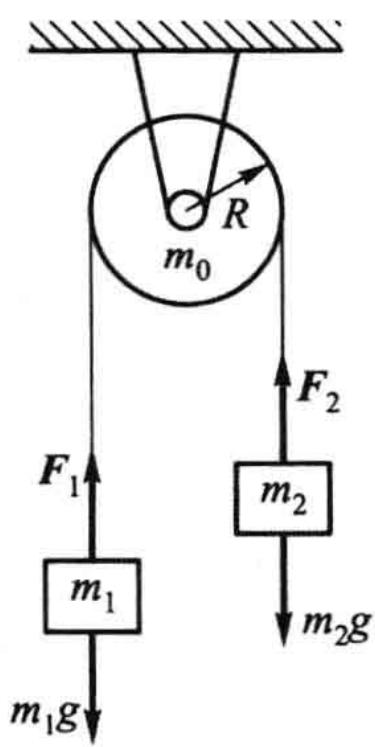
\includegraphics[width=0.18\textwidth]{figures/fig7-19.jpg}
  \end{figure}

\vfill

\textbf{7-20.}同一平面内的半径分别为 $R_{1}$ 和 $R_{2}$ , 质量分别为 $m_{1}$ 和 $m_{2}$ 的轮子以皮带相连接, 可绕各自的轴转动, 如习题 7-20 图所示。今在 $m_{1}$ 轮上作用一力矩 $M$ , 试求两轮的角加速度。设两轮的质量均集中在轮边, 皮带与轮之间无滑动, 皮带的质量和两轴承处的摩擦均可忽略。

\begin{figure}[H]
  \centering
  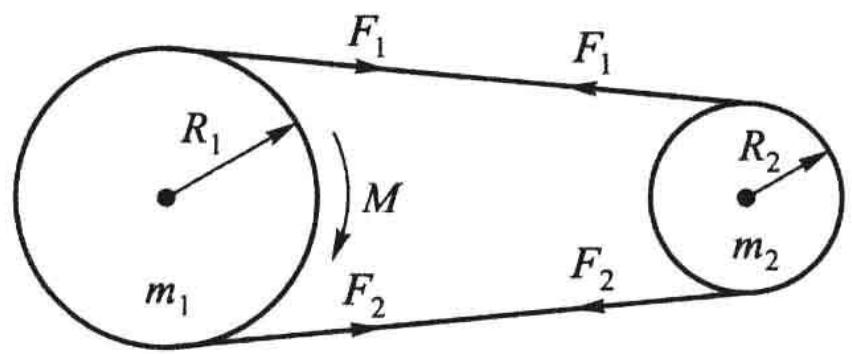
\includegraphics[width=0.35\textwidth]{figures/fig7-20.jpg}
  \end{figure}

\vfill
\newpage

\textbf{7-21.}一质量为 $m_{2}$ 、半径为 $R_{2}$ 的圆盘, 沿着绕在它边缘上的带子展开, 带子跨过一质量为 $m_{1}$ 、半径为 $R_{1}$ 的定滑轮, 带子的另一端悬挂一质量为 $m$ 的重物, 如习题 7-21 图所示。设圆盘沿竖直线下落, 假定皮带的质量可忽略。试求:

(1) 重物 m 的加速度 $a_{1}$ ;

(2) 圆盘质心的加速度 $a_{2}$ 。

\vfill

\textbf{7-22.}如习题 7-22 图所示, 一圆柱体沿倾角为 $\theta$ 的斜面滚下, 圆柱体与斜面之间的摩擦因数为 $\mu$ 。为使圆柱体沿斜面做纯滚动，试求 $\theta$ 的最大值。

\begin{figure}[H]
  \centering
  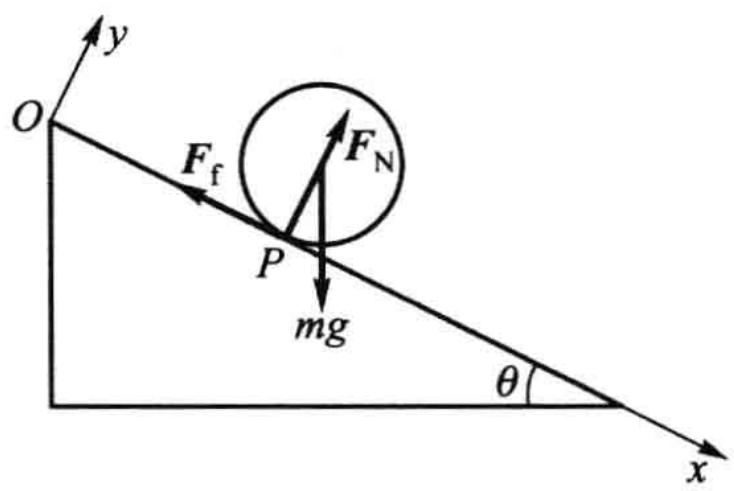
\includegraphics[width=0.3\textwidth]{figures/fig7-22.jpg}
  \end{figure}

\vfill
\newpage

\textbf{7-23.}如习题 7-23 图所示, 在倾角为 $\theta$ 的斜面上, 一质量为 $m$ 、半径为 $r$ 的圆柱体上绕有细绳,绳的一端缠绕在斜面顶端的定滑轮上,定滑轮为一质量为 $m_{0}$ 、半径也为 r 的圆盘。设圆柱体沿斜面滚下时细绳拉直且不能伸长,并与斜面平行,细绳与圆柱体及定滑轮之间无相对滑动,忽略滑轮轴承处的摩擦。

(1) 若圆柱体的滚动为纯滚动, 求其质心的加速度;

(2) 求圆柱体做纯滚动的条件。

\begin{figure}[H]
  \centering
  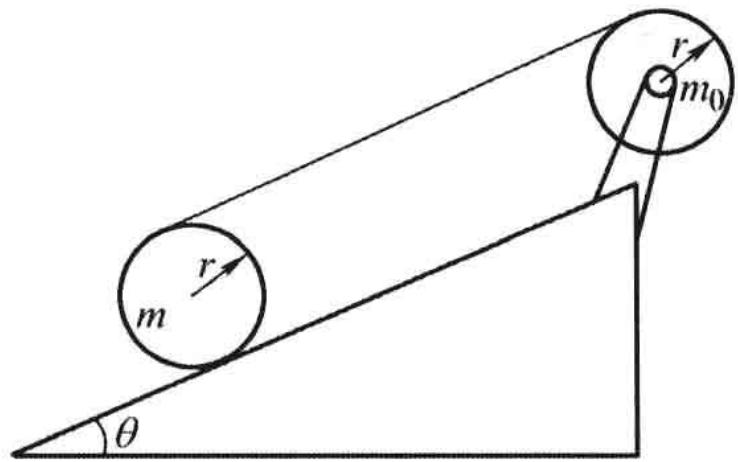
\includegraphics[width=0.3\textwidth]{figures/fig7-23_2.jpg}
  \end{figure}

\vfill

\textbf{7-24.}一质量为 $m_{0}$ , 半径为 $R$ 的均质圆盘, 可绕过其圆心且与盘面垂直的竖直轴自由转动。圆盘原来静止, 盘边上一质量为 $m$ 的人以恒定的相对于盘面的速度 $u$ 沿盘边缘行走时, 盘的转动角速度为多大?

\vfill
\newpage

\textbf{7-25.}一块半径为 $R$ 的水平轻质圆盘, 可绕过其圆心 $O$ 的竖直轴自由旋转。在圆盘下面的边缘处等间隔地系有四个质量都为 m 的小球, 如习题 7-25 图所示。开始时, 圆盘静止, 一辆质量也为 m 的玩具汽车从 O 出发, 以恒定的相对于盘的速率 $v_{0}$ 沿半径驶往盘边, 并沿盘边行驶。试求:

（1）当玩具汽车沿半径行驶时，圆盘的转动角速度 $\omega_{1}$ ;

(2) 当玩具汽车沿盘边行驶时, 圆盘的转动角速度 $\omega_{2}$ 。

\begin{figure}[H]
  \centering
  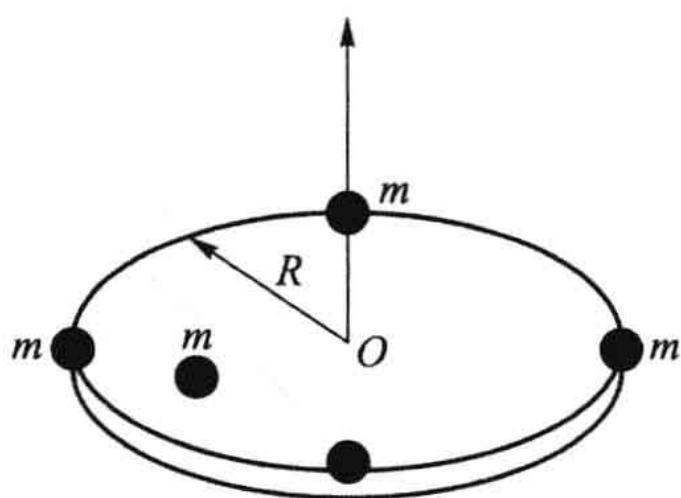
\includegraphics[width=0.25\textwidth]{figures/fig7-25_2.jpg}
  \end{figure}

\vfill

\textbf{7-26.}若上题中的竖直轴不在圆心, 而在某一小球位置处。玩具汽车从该轴处以恒定的相对于圆盘的速率 $v_{0}$ 沿盘边行驶。试求：

(1) 当玩具汽车行驶到第三小球位置处(即行驶了半圈)时,圆盘的转动角速度 $\omega_{1}$ ;

(2) 当玩具汽车行驶到第四小球位置处 (即行驶了 3/4 圈时), 圆盘的转动角速度 $\omega_{2}$ ;

(3) 当玩具汽车回到转轴处时, 圆盘的转动角速度 $\omega_{3}$ 。

\begin{figure}[H]
  \centering
  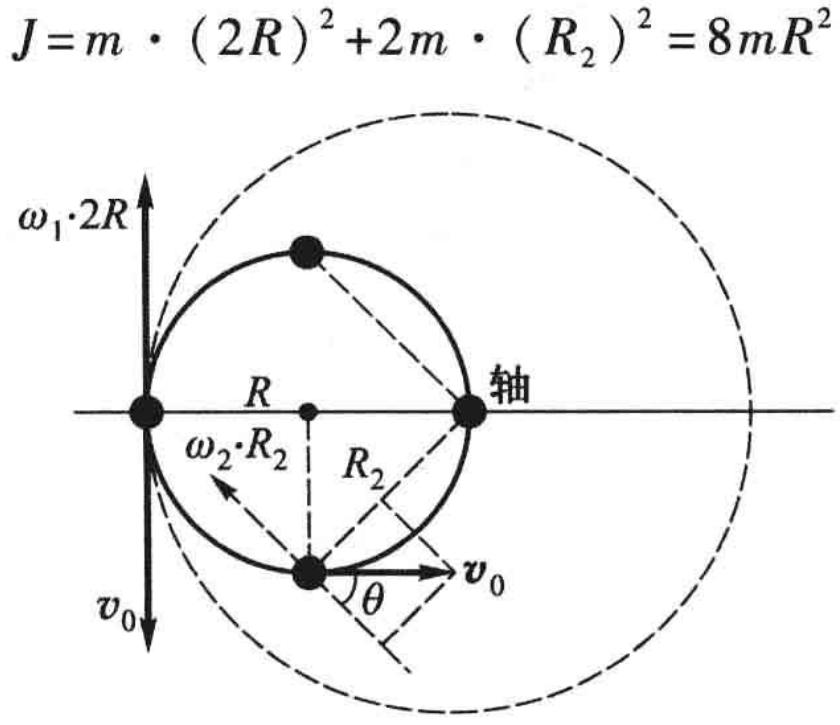
\includegraphics[width=0.3\textwidth]{figures/fig7-26_1.jpg}
  \end{figure}

\vfill
\newpage

\textbf{7-27.}质量皆为 $m$ 的两珠子可在光滑轻杆上自由滑动, 杆可在水平面内绕过 $O$ 点的光滑竖直轴自由旋转。原先两珠对称地位于 $O$ 点的两边, 与 $O$ 相距 $a$ , 在 $t = 0$ 时刻, 对杆施以冲量矩, 使杆在极短时间内即以角速度 $\omega_0$ 绕竖直轴旋转, 求 $t$ 时刻杆的角速度 $\omega$ 、角加速度 $\alpha$ 及两珠与 $O$ 点的距离 $r$ 。

\vfill

\textbf{7-28.}质量为 $m_{0}$ 、长为 $l$ 的均质细棒以一端为支点悬挂起来。一质量为 $m$ 的子弹以 $v_{0}$ 的水平速度射入棒的另一端，且留在棒内。试求在子弹射入棒后，棒的最大偏转角 $\theta$ 。设在棒偏转时，支点处的摩擦可忽略。

\vfill
\newpage

\textbf{7-29.}在一根长为 $3l$ 的轻杆上打一个小孔, 孔离一端的距离为 $l$ , 再在杆的两端以及距另一端为 $l$ 处各系一质量为 $m_0$ 的小球。然后通过此孔将杆悬挂于一光滑的水平细轴 $O$ 上, 如习题 7-29 图所示。开始时, 轻杆静止, 一质量为 $m$ 的小铅粒以 $v_0$ 的水平速度射入中间的小球, 并留在里面。若铅粒相对小球静止时杆的角位移可以忽略, 试求杆在以后摆动中的最大摆角。

\begin{figure}[H]
  \centering
  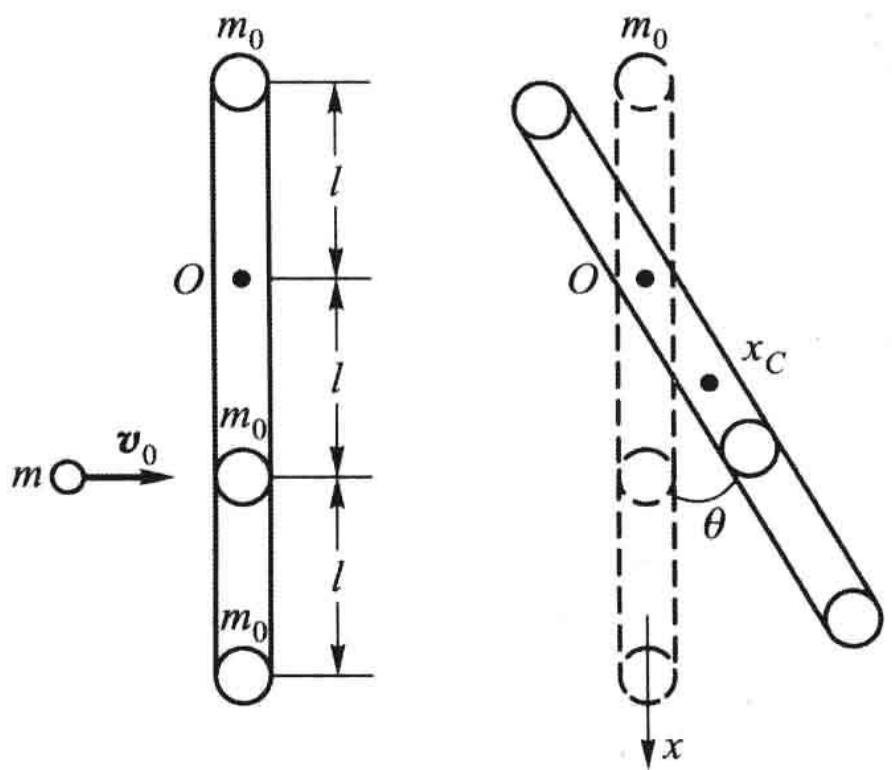
\includegraphics[width=0.3\textwidth]{figures/fig7-29.jpg}
  \end{figure}

\vfill

\textbf{7-30.}将一根长 $l$ 、质量为 $m_0$ 的均匀杆的一端搁在桌边, 另一端用手托住, 使杆处于水平位置, 如习题 7-30 图所示。试求将手释放瞬间杆对桌边的作用力。

\begin{figure}[H]
  \centering
  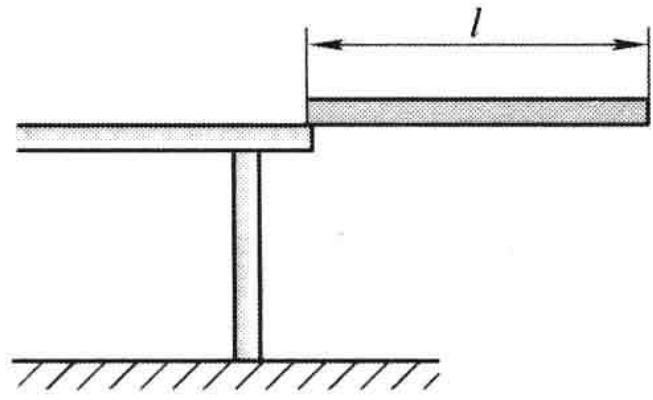
\includegraphics[width=0.3\textwidth]{figures/fig7-30.jpg}
  \end{figure}

\vfill
\newpage

\textbf{7-31.}两根质量均为 $m$ 、长均为 $l$ 的相同均匀杆，与一竖直轴刚性相连，杆与轴均成 $\theta$ 角,且三者在同一平面内,转轴被轴承在 A、B 点处固定,如习题 7-31 图所示。当转轴以恒定角速度 $\omega$ 转动时,求转轴对轴承的水平作用力。设两轴承到杆、轴连接点的距离均为 R。

\begin{figure}[H]
  \centering
  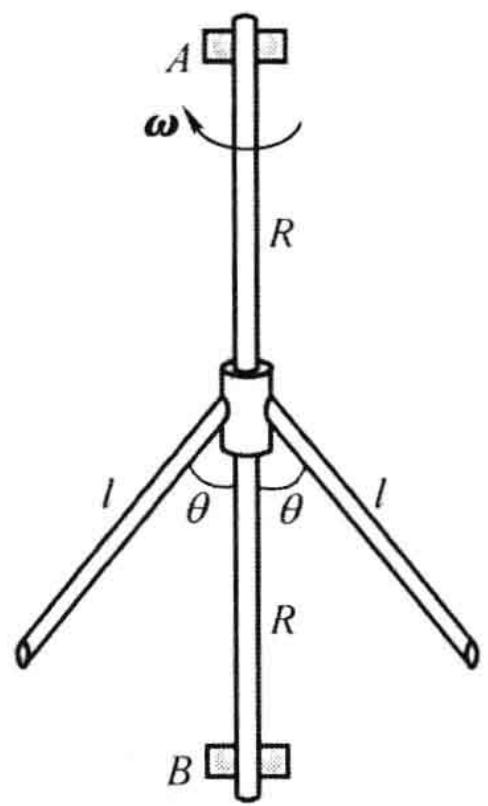
\includegraphics[width=0.2\textwidth]{figures/fig7-31.jpg}
  \end{figure}

\vfill

\textbf{7-32.}一直角尺由长度分别为 $a$ 和 $b$ 的两根棒构成, 能在竖直平面内绕过直角顶点的光滑水平轴自由转动,如习题7-32图所示。设长为 a 的棒与竖直线间的夹角为 $\alpha$ 。开始时,将尺拉至 $\alpha=0$ 位置,然后由静止开始释放。求 $\alpha$ 的最大值。

\begin{figure}[H]
  \centering
  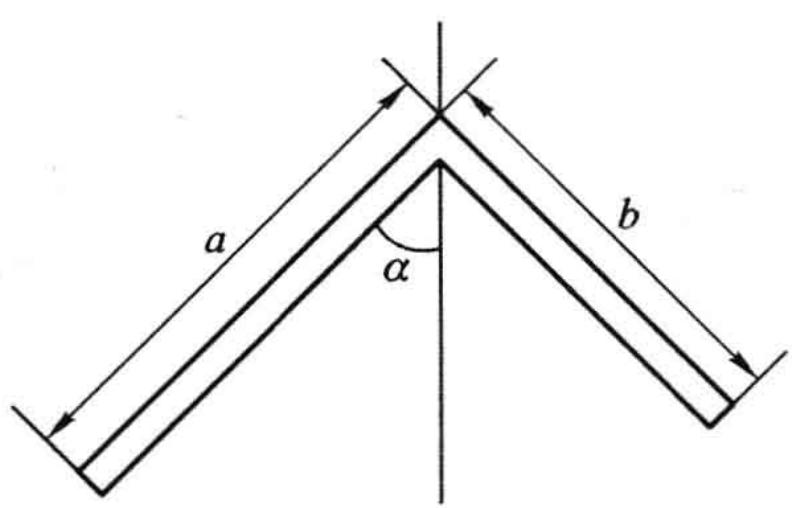
\includegraphics[width=0.3\textwidth]{figures/fig7-32.jpg}
  \end{figure}

\vfill
\newpage

\textbf{7-33.}质量为 $m$ 的板受水平力 $F$ 的作用沿水平面运动, 板与水平面之间的摩擦因数为 $\mu$ 。板上放着质量为 $m_{0}$ 、半径为 $R$ 的圆柱体, 如习题 7-33 图所示。

(1) 若圆柱体在板上的运动为纯滚动, 求板的加速度。

(2) 为使圆柱体做纯滚动, 求 $F$ 的最大值。设圆柱体与板之间的摩擦因数也是 $\mu$ 。

\begin{figure}[H]
  \centering
  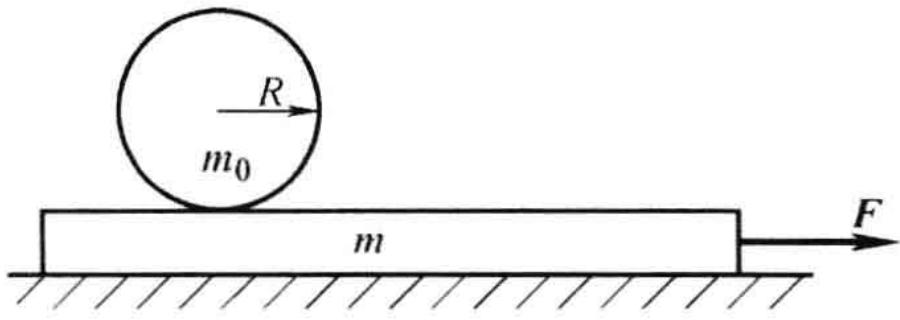
\includegraphics[width=0.4\textwidth]{figures/fig7-33_1.jpg}
  \end{figure}

\vfill

\textbf{7-34.}一根长为 $l$ 、质量为 $m$ 的均匀细棒, 放置在光滑的水平桌面上, 一个水平的冲量 $I$ 突然垂直地作用于棒的另一端。试问:

(1) 当棒旋转了 $360^{\circ}$ 时, 其质心运动了多远?

(2) 冲击后棒的动能为多大?

\vfill
\newpage

\textbf{7-35.}如习题 7-35 图所示, 一质量为 $m$ 、半径为 $r$ 的小球, 从高为 $h_0$ 的斜坡顶端由静止开始滚下, 并从高为 $h(h < h_0)$ 的斜坡的另一端飞离。离开时, 小球的速度为竖直向上, 若小球与斜坡之间的摩擦因数足够大, 使小球始终做纯滚动, 求小球飞离后所能上升的最大高度。

\begin{figure}[H]
  \centering
  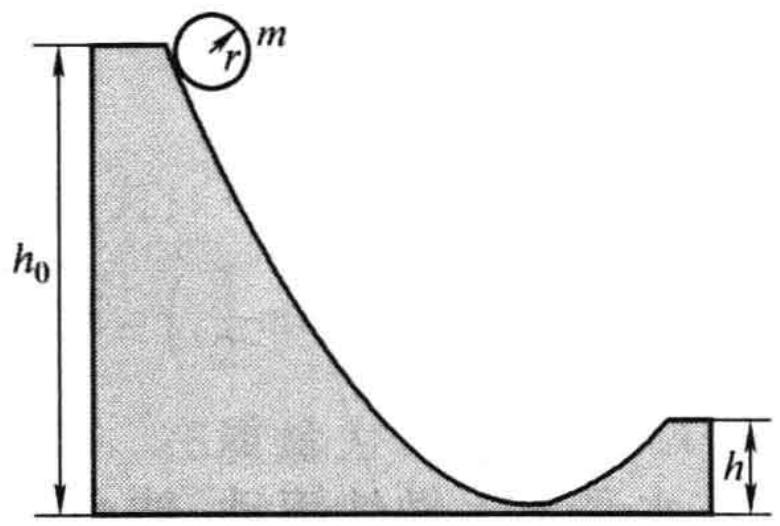
\includegraphics[width=0.3\textwidth]{figures/fig7-35.jpg}
  \end{figure}

\vfill

\textbf{7-36.}将一水平方向上的冲量 $I$ 作用在质量为 $m_{0}$ 、半径为 $R$ 的最初是静止的均质小球上, 作用点位于球心的上方, 距地面的高度为 $h$ , 作用线位于过球心而平行于纸面的平面内, 如习题 7-36 图所示。试分析小球以后的运动情况, 并

求出小球做纯滚动时的角速度 $\omega$ 。

\vfill
\newpage

\textbf{7-37.}一质量为 $m$ 、半径为 $r$ 的均质球 1 在水平面上做纯滚动, 球心速度为 $v_{0}$ , 与另一完全相同的静止球 2 发生对心碰撞, 如习题 7-37 图所示。设碰撞时各接触面间的摩擦均可忽略, 碰撞是弹性的。

（1）碰撞后，各自经过一段时间，两球开始做纯滚动，求出此时各球心的速度；

(2) 求此过程中系统机械能的损失。

\begin{figure}[H]
  \centering
  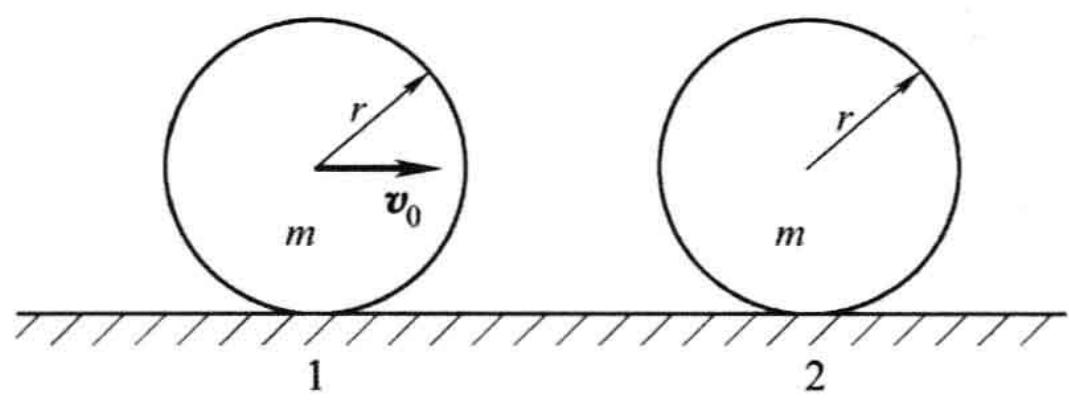
\includegraphics[width=0.35\textwidth]{figures/fig7-37.jpg}
  \end{figure}

\vfill

\textbf{7-38.}在质量为 $m$ 、边长为 $a$ 的正方形板的一个顶点上系一根绳, 绳的长度也是 $a$ , 其另一端与光滑墙面相连。把板的另一顶点靠在墙上, 使绳与板平面处在同一与墙面垂直的竖直平面内, 如习题 7-38 图所示。求平衡时绳中的张力。

\begin{figure}[H]
  \centering
  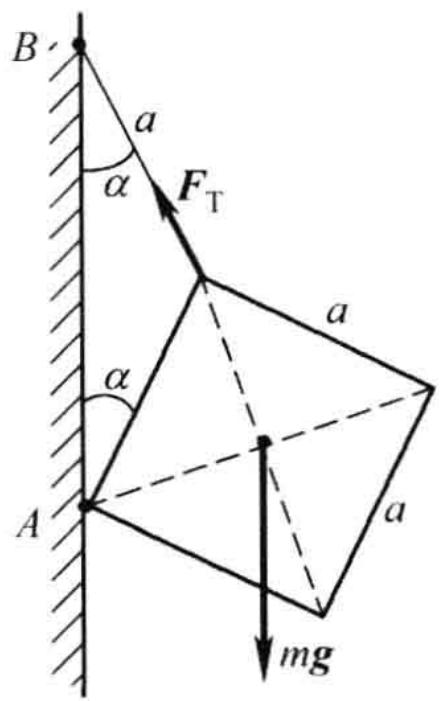
\includegraphics[width=0.2\textwidth]{figures/fig7-38.jpg}
  \end{figure}

\vfill
\newpage

\textbf{7-39.}质量为 $m$ 的线轴如习题 7-39 图所示, 其外半径为 $a$ , 绕线部分的半径为 $b$ , 设其绕轴线的转动惯量为 $J$ 。今将绕线的一端以一恒力 $F$ 拉它, $F$ 与水平面成 $\theta$ 角, 设 $F \sin \theta < mg$ 。

(1) 为使线轴向后 (即与 $F$ 的水平分量方向相反) 做纯滚动,

(i) 求 $\theta$ 的范围；

(ii) 若满足(i)中的条件,则摩擦因数 $\mu$ 至少应为多大?

(iii) 求出线轴质心运动的加速度。

(2) 为使线轴向前做纯滚动, 同样求出 (1) 中的三个问题。

\vfill

\textbf{7-40.}一质量为 $m$ 、半径为 $R$ 的圆盘可绕通过其中心 $O$ 的竖直轴以 $\omega$ 角速度转动,如习题7-40图所示。试求轴承处所受的水平作用力,设OA=OB=l,垂直于圆盘表面的法线与竖直轴成 $\alpha$ 角。

\begin{figure}[H]
  \centering
  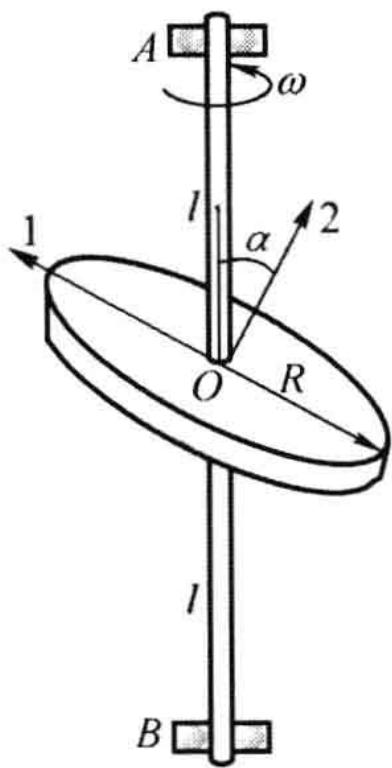
\includegraphics[width=0.2\textwidth]{figures/fig7-40.jpg}
  \end{figure}

\vfill
\newpage

\textbf{7-41.}如习题 7-41 图所示,一陀螺由一质量为 $m$ 、半径为 $R$ 的厚圆盘构成,通过圆心且垂直于圆盘的自转轴为一轻杆,杆的尖端自由地支在离盘质心为 l 处的枢纽上。现陀螺绕自转轴以 $\omega_{0}$ 的角速度高速自转,其自转轴以与水平面成 $\theta$ 角做均匀进动。试求:(1) 进动角速度;(2) 枢纽所受的力。

\begin{figure}[H]
  \centering
  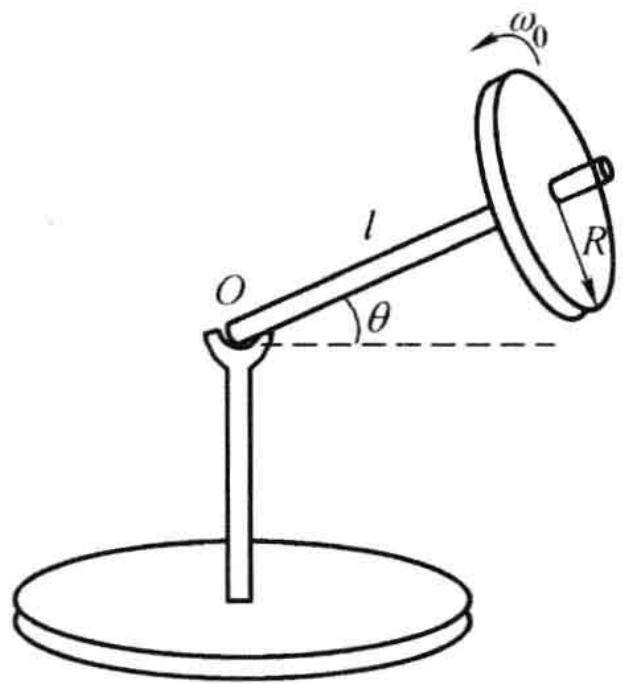
\includegraphics[width=0.25\textwidth]{figures/fig7-41.jpg}
  \end{figure}

\vfill

\textbf{7-42.}一半径为 $r$ 的硬币,在桌面上绕半径为 $R$ 的圆滚动,其质心速度为 $v$ , 如习题 7-42 图(a)所示。设硬币的滚动为纯滚动。求其轴线与水平线所成的角 $\theta(\theta<<1,R>>r)$ 。

\begin{figure}[H]
  \centering
  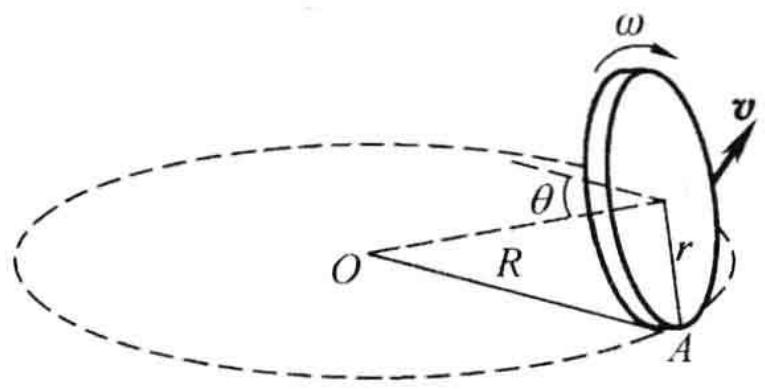
\includegraphics[width=0.3\textwidth]{figures/fig7-42_a.jpg}
  \end{figure}

\vfill
\newpage

\textbf{7-43.}一陀螺由半径为 $R$ 、质量为 $m$ 的薄圆盘及过其圆心且垂直于盘面的轻杆组成, 盘缘及杆的一端 $O$ 靠在桌面上, 杆与桌面成 $45^{\circ}$ 角, 如习题 7-43 图 (a) 所示。今陀螺以杆的一端 $O$ 为支点, 靠在桌面上做无滑滚动, 使杆绕竖直轴做匀速转动, 角速度为 $\Omega$ 。求:

(1) 桌面对盘缘的支承力 $F_{N}$ ;

(2) 陀螺的动能。

\begin{figure}[H]
  \centering
  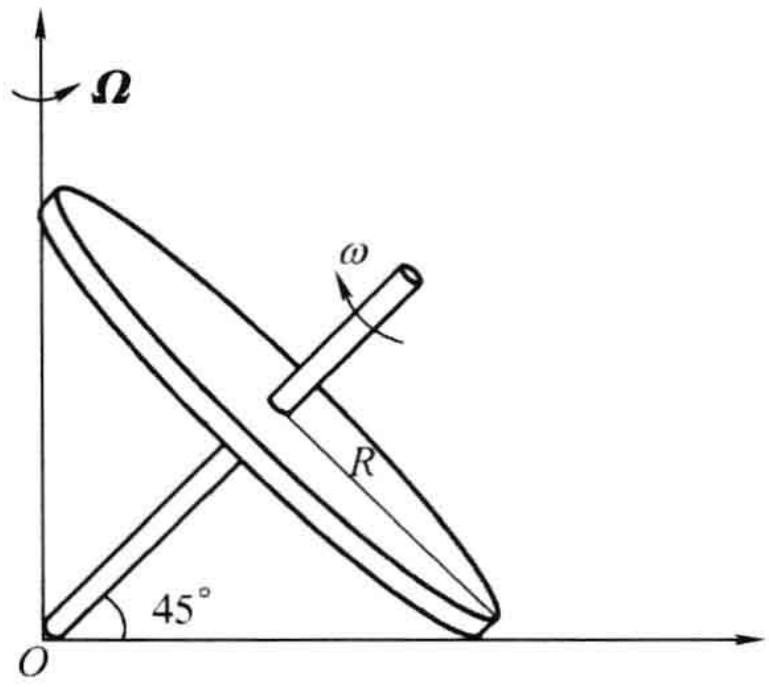
\includegraphics[width=0.3\textwidth]{figures/fig7-43_a.jpg}
\end{figure}

\vfill
\newpage

\textbf{8-1.}在如习题 8-1 图所示的装置中, 已知容器与容器内液体的总质量为 $5.0 \mathrm{~kg}$ , 吊在弹簧秤下的重物是边长为 $8.0 \mathrm{~cm}$ 的立方体, 弹簧秤的读数为 $6.0 \mathrm{~kg}$ , 台秤的读数为 $8.1 \mathrm{~kg}$ 。求: 

(1) 重物的质量; 

(2) 容器内液体的密度。

\begin{figure}[H]
  \centering
  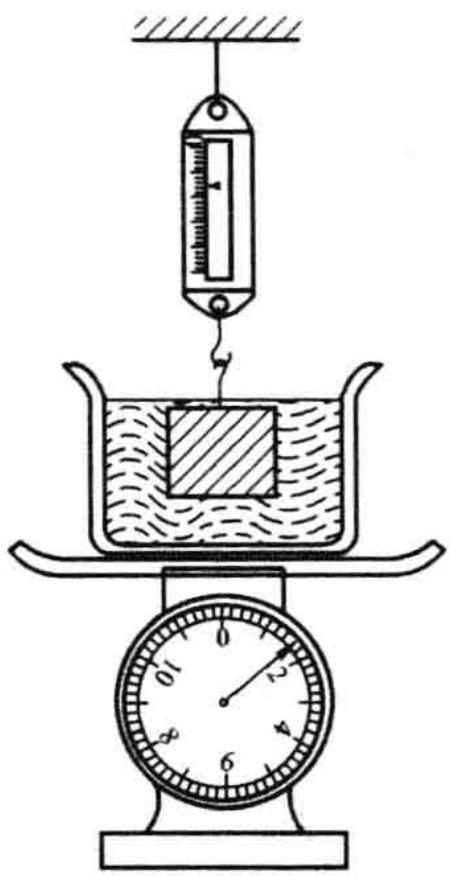
\includegraphics[width=0.15\textwidth]{figures/fig8-1.jpg}
  \end{figure}

\vfill

\textbf{8-2.}一根横截面积 $S_{1} = 5.00 \mathrm{~cm}^{2}$ 的细管, 连接在一个容器上, 容器的横截面积 $S_{2} = 100 \mathrm{~cm}^{2}$ , 高度 $h_{2} = 5.00 \mathrm{~cm}$ 。把水注入, 使水至容器底部的高度 $h_{1} + h_{2} = 100 \mathrm{~cm}$ , 如习题 8-2 图所示。求:

(1) 水对容器底部的作用力为多大?

(2) 此装置内水的重力为多大?

(3) 解释(1)、(2)所求得的结果为何不同?

\begin{figure}[H]
  \centering
  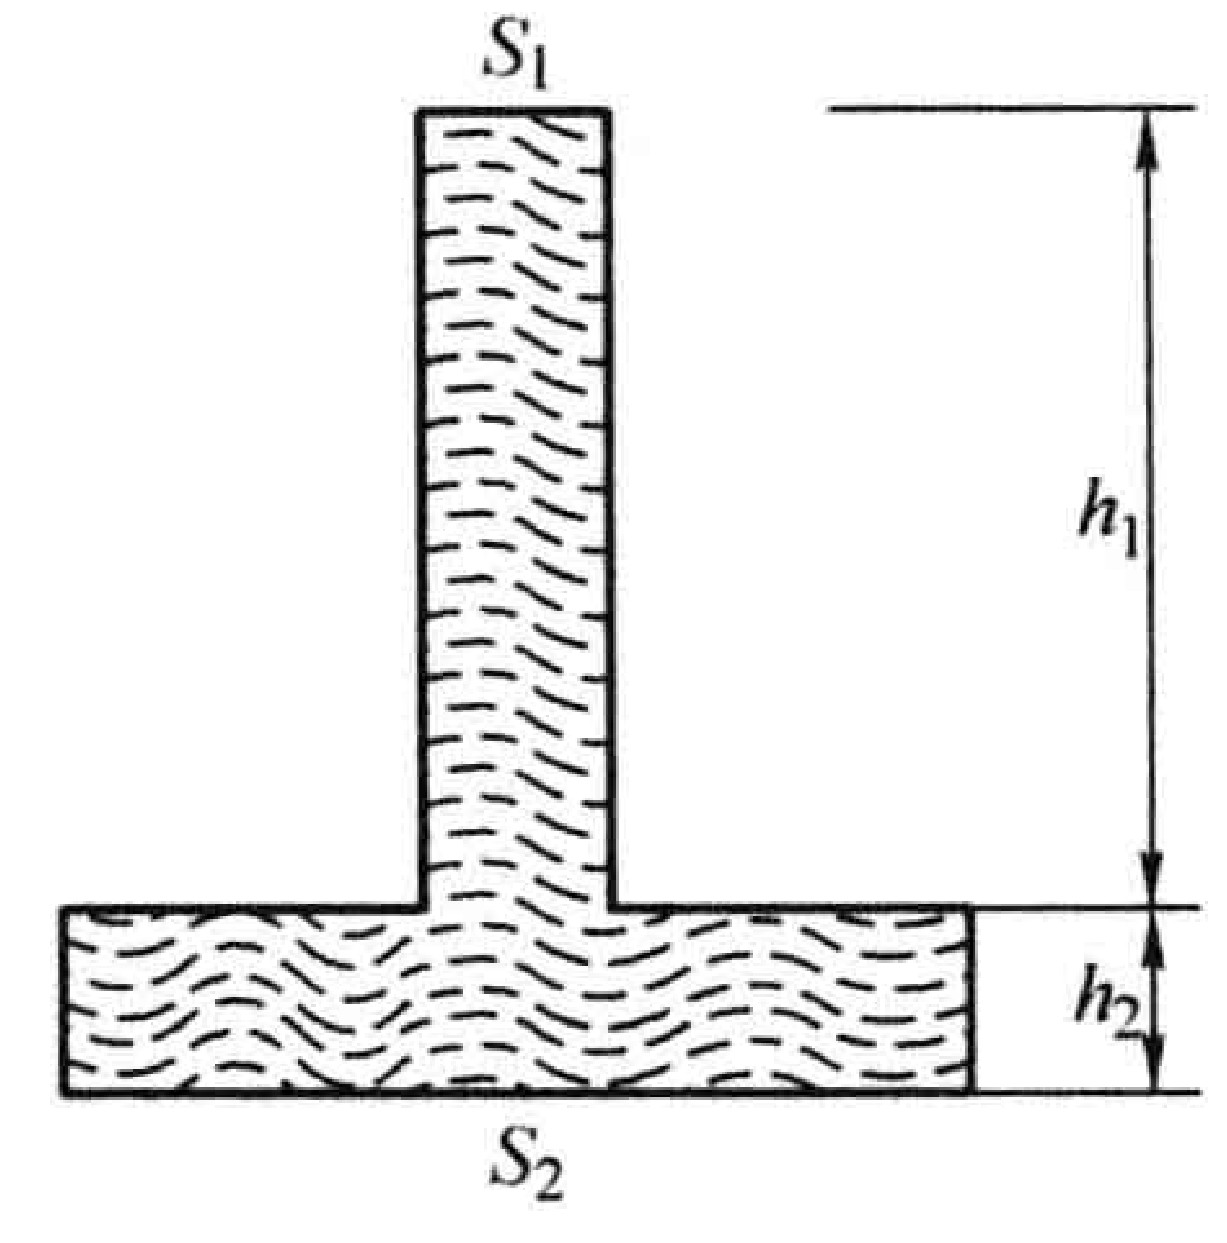
\includegraphics[width=0.25\textwidth]{figures/fig8-2.jpg}
  \end{figure}

\vfill
\newpage

\textbf{8-3.}一根长为 $l$ 、密度为 $\rho$ 的均质细杆, 浮在密度为 $\rho_{0}$ 的液体里。杆的一端由一竖直细绳悬挂着,使该端高出液面的距离为d,如习题8-3图所示。试求:(1)杆与液面的夹角 $\theta$ ;(2)绳中的张力 $F_{T}$ 。设杆的横截面积为S。

\begin{figure}[H]
  \centering
  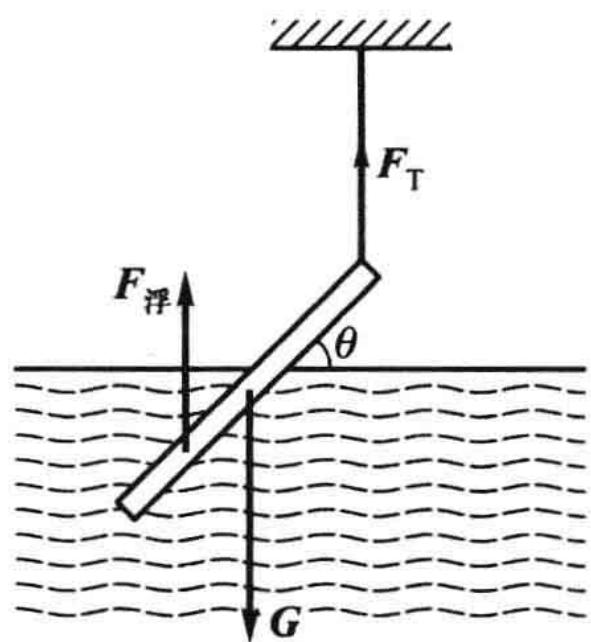
\includegraphics[width=0.25\textwidth]{figures/fig8-3.jpg}
  \end{figure}

\vfill

\textbf{8-4.}若上题中细杆的一端由一竖直细绳与装液体的容器底面相连, 使该端低于液面的距离为 $d$ , 如习题 8-4 图所示。求解上题中的两个问题。

\begin{figure}[H]
  \centering
  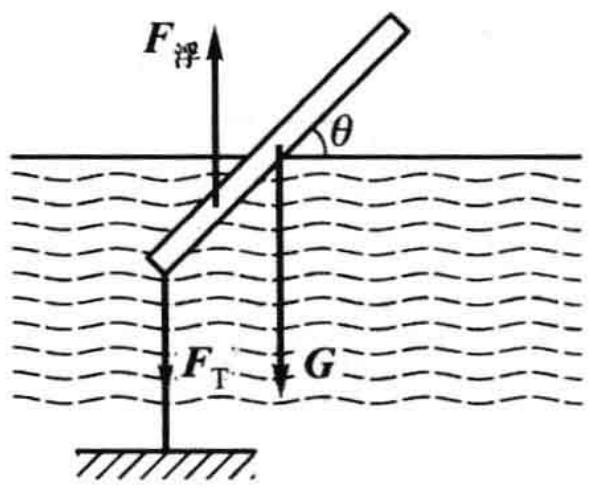
\includegraphics[width=0.25\textwidth]{figures/fig8-4.jpg}
  \end{figure}

\vfill
\newpage

\textbf{8-5.}一粗细均匀的 U 形管内装有一定量的液体。U 形管底部的长度为 $l$ 。当 U 形管以加速度 $a$ 沿水平方向加速时, 如习题 8-5 图所示, 求两管内液面的高度差 $h$ 。
\begin{figure}[H]
  \centering
  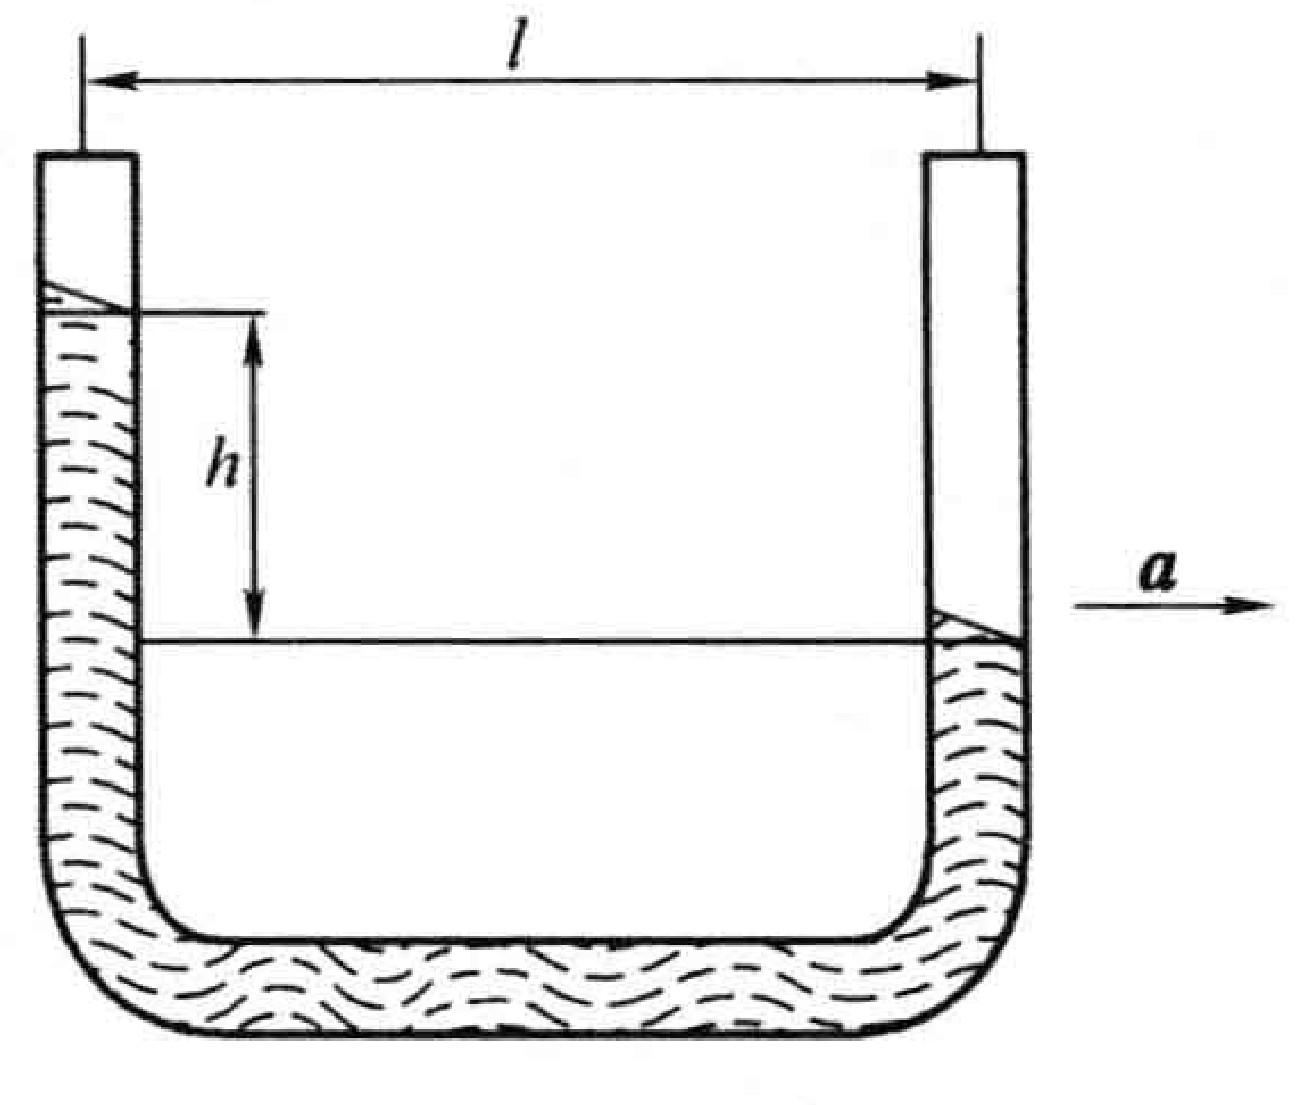
\includegraphics[width=0.25\textwidth]{figures/fig8-5.jpg}
  \end{figure}

\vfill

\textbf{8-6.}一立方体钢块平正地浮在容器内的水银中。已知钢块的密度为 $7.8 \mathrm{~g} / \mathrm{cm}^{3}$ , 水银的密度为 $13.6 \mathrm{~g} / \mathrm{cm}^{3}$ 。

(1) 问钢块露出水银面之上的高度与边长之比为多大?

(2) 如果在水银面上加水,使水面恰与钢块的顶相平,问水层的厚度与钢块边长的比例为多大?

\vfill
\newpage

\textbf{8-7.}利用一根跨过水坝的粗细均匀的虹吸管,从水库里取水,如习题 8-7 图所示,已知水库的水位的深度 $h_A = 2.00 \mathrm{~m}$ , 虹吸管出水口的高度 $h_B = 1.00 \mathrm{~m}$ , 坝高 $h_C = 2.50 \mathrm{~m}$ 。设水在虹吸管内做定常流动。

(1) 求 A、B、C 三个位置处的压强；

(2) 若虹吸管的横截面积为 $7.00 \times 10^{-4} \mathrm{~m}^{2}$ , 求水从虹吸管流出的体积流量。

\begin{figure}[H]
  \centering
  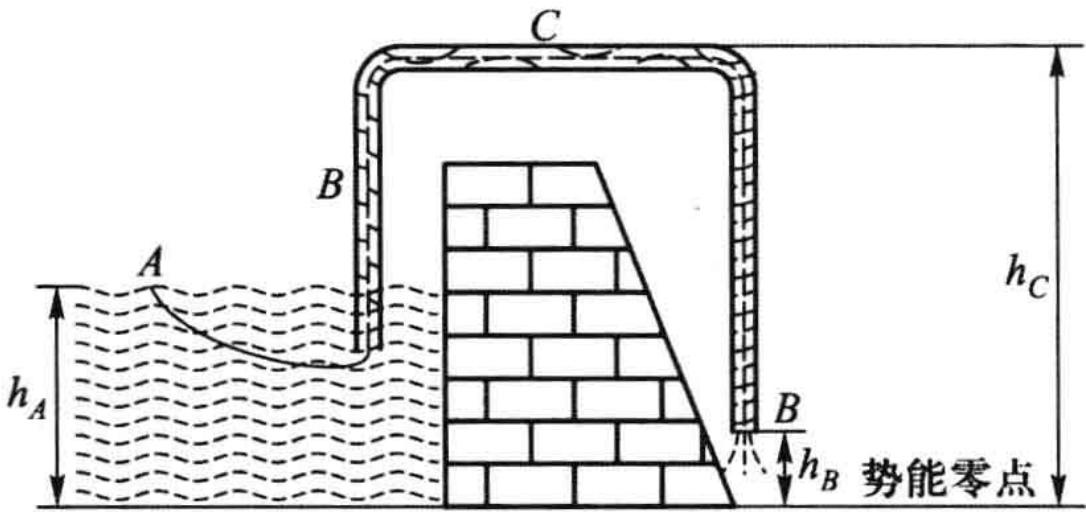
\includegraphics[width=0.4\textwidth]{figures/fig8-7.jpg}
  \end{figure}

\vfill

\textbf{8-8.}如习题 8-8 图所示,一水平管下面装有一 U 形管,U 形管内盛有水银。已知水平管中粗、细处的横截面积分别为, $S_{A}=5.0 \times 10^{-3} \mathrm{~m}^{2}, S_{B}=1.0 \times 10^{-3} \mathrm{~m}^{2}$ 。当水平管中有水流做定常流动时,测得 U 形管中水银面的高度差为 $h=3.0 \times 10^{-2} \mathrm{~m}$ 。求水流在粗管处的流速 $v$ 。已知水和水银的密度分别为 $\rho=1.0 \times 10^{3} \mathrm{~kg/m}^{3}, \rho'=13.6 \times 10^{3} \mathrm{~kg/m}^{3}$ 。

\begin{figure}[H]
  \centering
  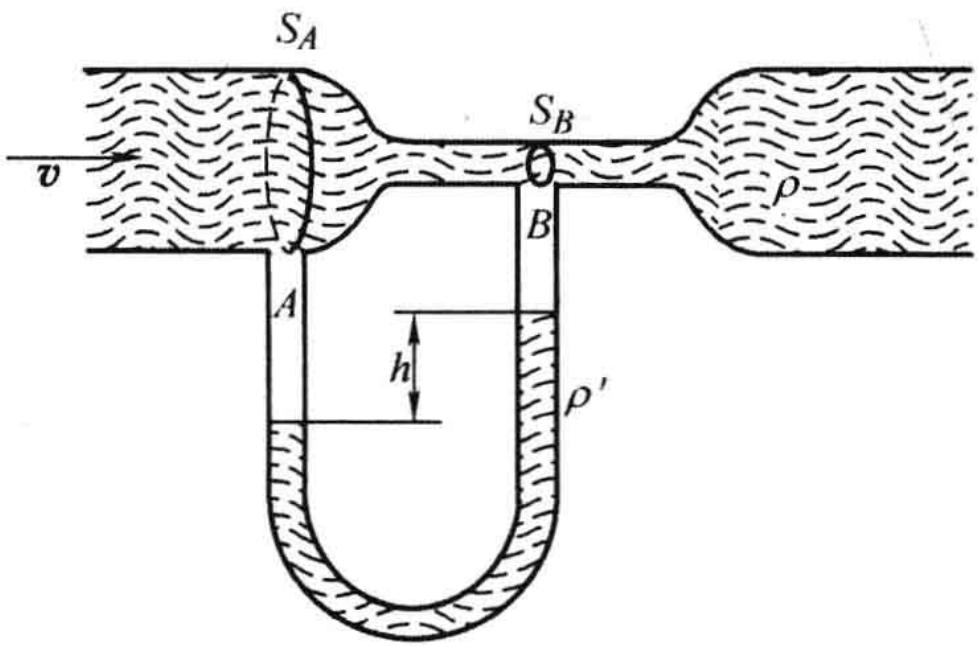
\includegraphics[width=0.4\textwidth]{figures/fig8-8.jpg}
  \end{figure}

\vfill
\newpage

\textbf{8-9.}利用压缩空气把水从一密封的容器内通过一管子压出,如习题 8-9 图所示。已知管子的出口处比容器内水面高 $h = 0.50 \mathrm{~m}$ 。当水从管口以 $1.5 \mathrm{~m} / \mathrm{s}$ 的流速流出时，求容器内空气的压强。

\begin{figure}[H]
  \centering
  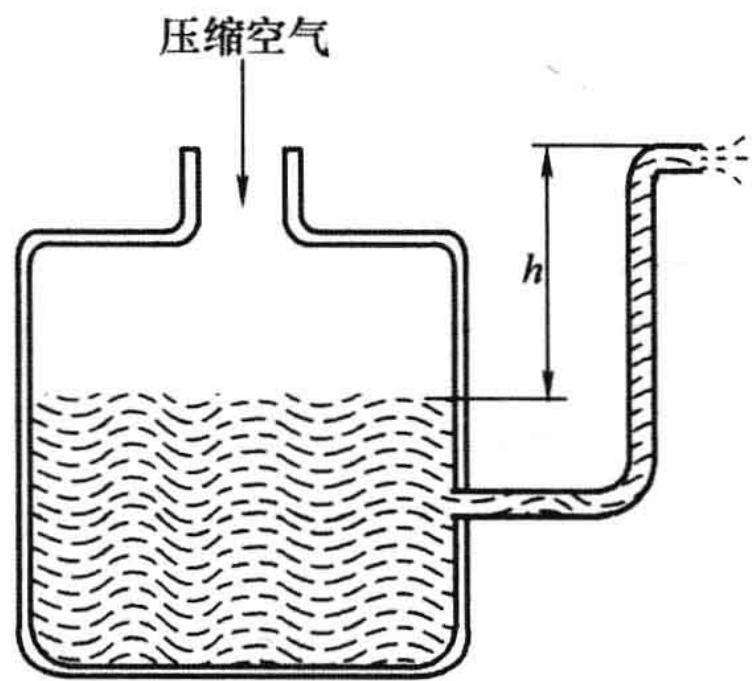
\includegraphics[width=0.35\textwidth]{figures/fig8-9.jpg}
  \end{figure}

\vfill

\textbf{8-10.}一喷泉竖直喷出高度为 $H$ 的水流, 喷泉的喷嘴具有上细下粗的截锥形状。上截面的直径为 $d_{1}$ , 下截面的直径为 $d_{2}$ , 喷嘴高为 $h$ 。设大气压强为 $p_{0}$ , 求:

(1) 水的体积流量；

(2) 喷嘴下截面处的压强。

\vfill
\newpage

\textbf{8-11.}如习题 8-11 图所示, 在一大容器的底部接一竖直管, 在 $B$ 处装有一压力计竖直管的下口 $C$ 处用软木塞塞住。若 $A$ （容器内液面处）、$B$ 、$C$ 三点的高度分别为 $h_A,h_B,h_C$ 。求:

(1) 此时压力计中液面的高度 $h_{1}$ ;

(2) 拔去软木塞, 当水做定常流动后, 压力计中液面的高度 $h_{2}$ 。

\begin{figure}[H]
  \centering
  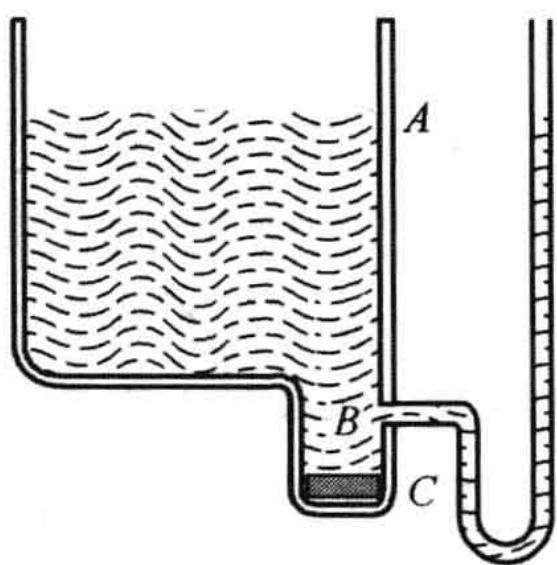
\includegraphics[width=0.25\textwidth]{figures/fig8-11.jpg}
  \end{figure}

\vfill

\textbf{8-12.}在一截锥形容器内盛有高度为 $h = 0.7 \mathrm{~m}$ 的水, 其侧壁与底面成 $\theta = 60^{\circ}$ 角, 容器被放在高为 $h_0 = 0.50 \mathrm{~m}$ 的物体上, 在容器壁的底部开有一小孔, 如习题 8-12 图所示。求水从小孔射出后的水平射程 $L$ 。

\begin{figure}[H]
  \centering
  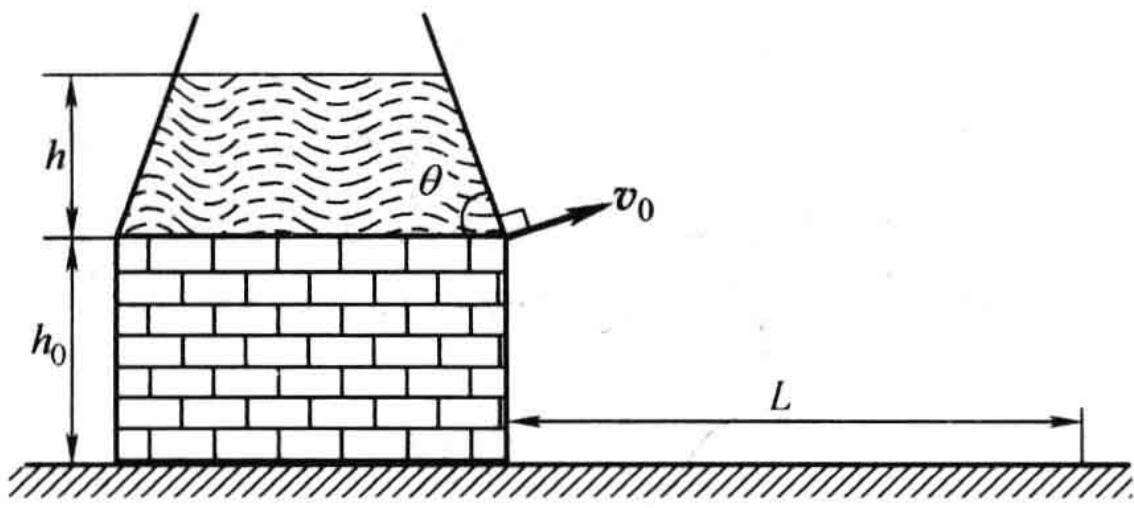
\includegraphics[width=0.35\textwidth]{figures/fig8-12.jpg}
  \end{figure}

\vfill
\newpage


\textbf{8-13.}在某水池的边上装有一宽为 $1.0 \mathrm{~m}$ , 高为 $2.0 \mathrm{~m}$ 的小门, 其下边与水池底相平, 并用铰链与池壁连接。试问, 当池内的水深刚好没过门时, 门受到的水的作用力相对于铰链的力矩为多大?

\begin{figure}[H]
  \centering
  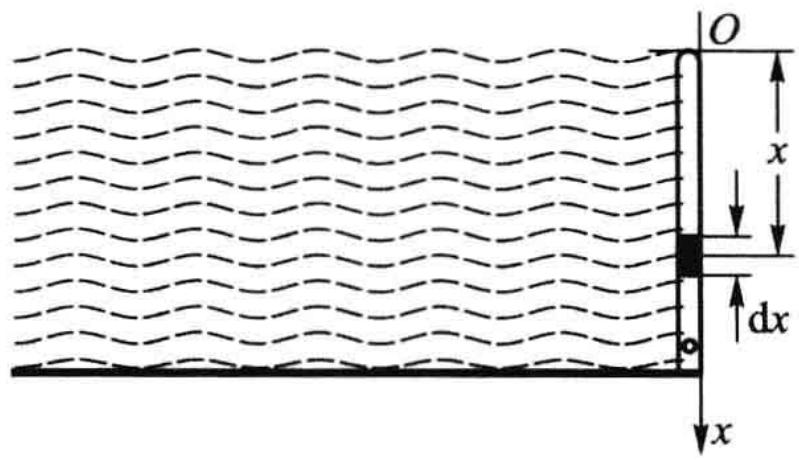
\includegraphics[width=0.35\textwidth]{figures/fig8-13.jpg}
  \end{figure}

\vfill

\textbf{8-14.}在一直径很大的圆柱形水桶壁的近底部处有一个直径为 $0.04 \mathrm{~m}$ 的小孔。若桶内水的深度为 $1.60 \mathrm{~m}$ 。

(1) 求此时水从小孔中流出的体积流量 $Q_{1}$ 。

(2) 若小孔为薄壁圆孔, 其收缩系数为 $61\%$ 。求实际的体积流量 $Q_{2}$ , 并求由于收缩现象的存在而造成的计算值与实际值之间的百分误差。

\vfill
\newpage

\textbf{8-15.}液体在一水平管道中流动, $A$ 处和 $B$ 处的横截面积分别为 $S_A$ 和 $S_B$ , $B$ 管口与大气相通, 压强为 $p_0$ , 若在 $A$ 处用一细管与容器相通, 如习题 8-15 图所示, 试证明: 当 $h$ 满足下式 $h = \frac{Q^2}{2g}\left(\frac{1}{S_A^2} - \frac{1}{S_B^2}\right)$ 时, $A$ 处的压强刚好能将比水平管低 $h$ 处的同种液体吸上来。其中 $Q$ 为体积流量。

\begin{figure}[H]
  \centering
  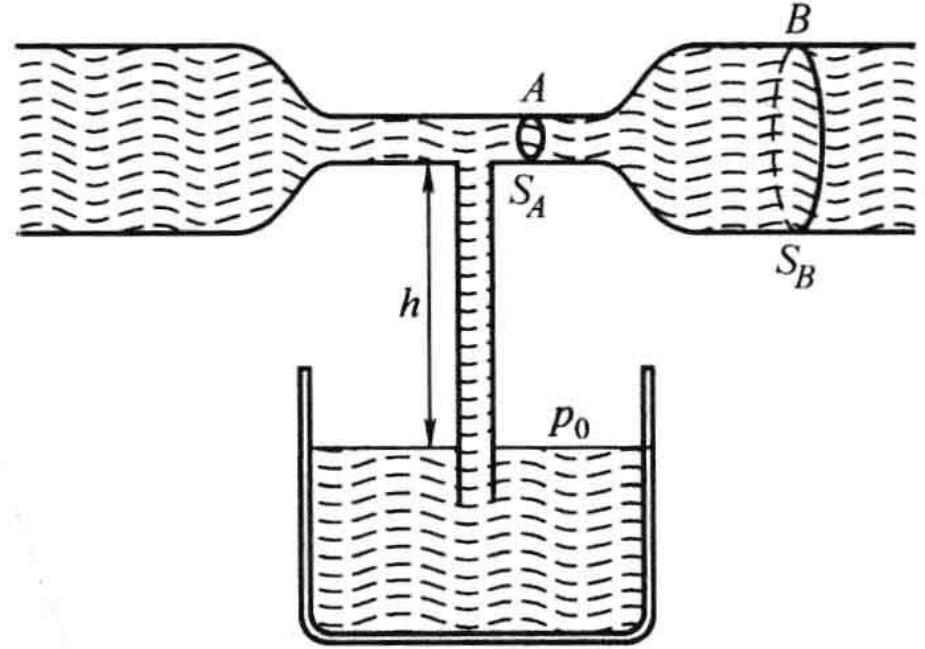
\includegraphics[width=0.25\textwidth]{figures/fig8-15.jpg}
  \end{figure}

\vfill

\textbf{8-16.}在一大容器的底部有一小孔, 容器横截面积与小孔面积之比为 100, 容器内盛有高度 $h = 0.80 \mathrm{~m}$ 的水。求容器内水流完所需的时间。设在整个过程中, 水的流动可视为定常流动。

\vfill
\newpage

\textbf{8-17.}一根长为 $L$ 的水平粗管与一根竖直细管连接成如习题8-17图所示的形状。把细管的下端插入密度为 $\rho_{\mathrm{f}}$ 的液体中，然后将粗管的管口封住，并使其绕细管以恒定的角速度 $\omega$ （很小）旋转，如习题8-17图所示。已知粗管在绕轴旋转之前，其内空气的密度为 $\rho_{\mathrm{a}}$ ，压强为$p_{a}$ 。设细管的体积与粗管相比可以忽略,忽略毛细现象和旋转前后管内空气密度的变化。求细管中液体上升的高度 h 。设温度不变。

\begin{figure}[H]
  \centering
  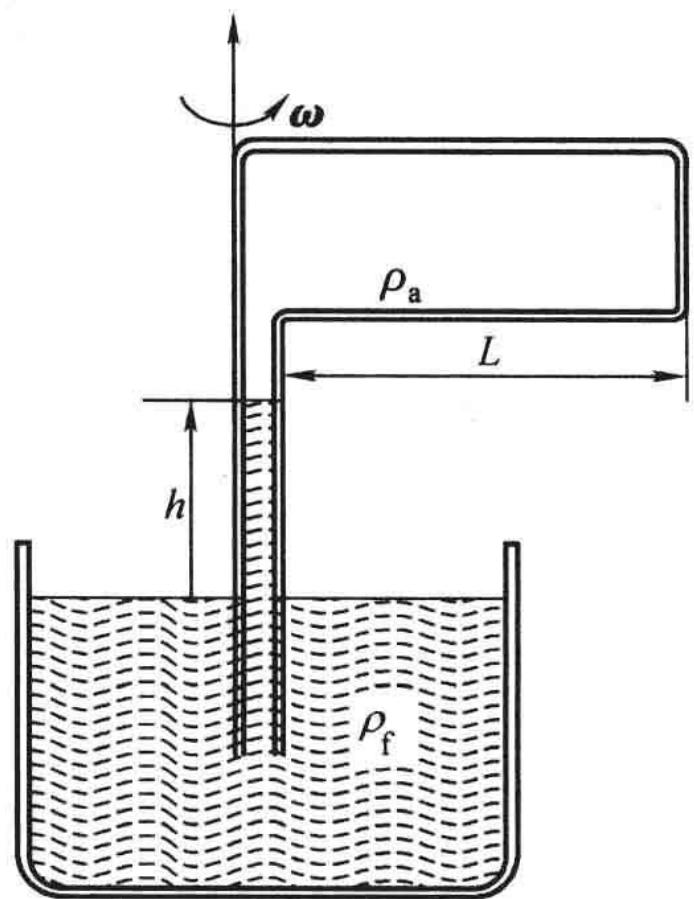
\includegraphics[width=0.25\textwidth]{figures/fig8-17.jpg}
  \end{figure}

\vfill

\textbf{8-18.}一个半径 $r = 0.20 \times 10^{-2} \mathrm{~m}$ 的小球落入 $\rho = 0.90 \times 10^{3} \mathrm{~kg} / \mathrm{m}^{3}$ 的黏性液体中。已知小球的密度 $\rho' = 6.5 \times 10^{3} \mathrm{~kg} / \mathrm{m}^{3}$ , 并测得小球在该液体中的最终速度 $v_{\mathrm{f}} = 0.24 \mathrm{~m} / \mathrm{s}$ 。试求:

(1) 液体的黏度 $\eta$ ;

(2) 小球在下降过程中加速度为 $\frac{1}{3} g$ 时刻的速度 $v$ 。


\vfill
\newpage

\textbf{9-1.}一质点沿 $x$ 轴做简谐振动, 其运动方程为 $x = 0.4 \cos \left[3 \pi \left(t + \frac{1}{6}\right)\right]$ , 式中 $x$ 和 $t$ 的单位分别为 $\mathbf{m}$ 和 $\mathbf{s}$ 。求:

(1) 振幅、周期和角频率；

(2) 初相位、初位移和初速度；

(3) t=1.5 s 时的位移、速度和加速度。

\vfill

\textbf{9-2.}一质点做振幅 $A = 0.30 \mathrm{~m}$ 的简谐振动。当质点的位移 $x = 0.15 \mathrm{~m}$ 时的速度大小为 $v = 0.9 \mathrm{~m} / \mathrm{s}$ , 求振动频率 $\nu$ 。

\vfill
\newpage

\textbf{9-3.}一质点做正弦简谐振动, 在某相位时, 其位移为 $x_0$ , 当相位增大一倍时, 其位移为 $\sqrt{3} x_0$ 。求振幅 $A$ 。

\vfill

\textbf{9-4.}一根质量为 $m$ 的均匀杆, 放在两个完全相同的轮子上, 两轮心间距离为 $2l$ , 并沿习题 9-4 图 (a) 所示的方向高速旋转, 杆与轮子间的摩擦因数为 $\mu$ , $t = 0$ 时, 杆静止, 杆的质心与两轮中间点的距离为 $x_0$ 。

(1) 证明杆沿水平方向将做简谐振动,并求出振动的角频率;

(2) 若两轮均沿与习题 9-4 图(a)所示的相反方向旋转, 求杆的质心从 $x_{0}$ 运动到任意一点 $x$ ( $x$ 表示杆的质心与两轮中间点的距离)时所用的时间。

\begin{figure}[H]
  \centering
  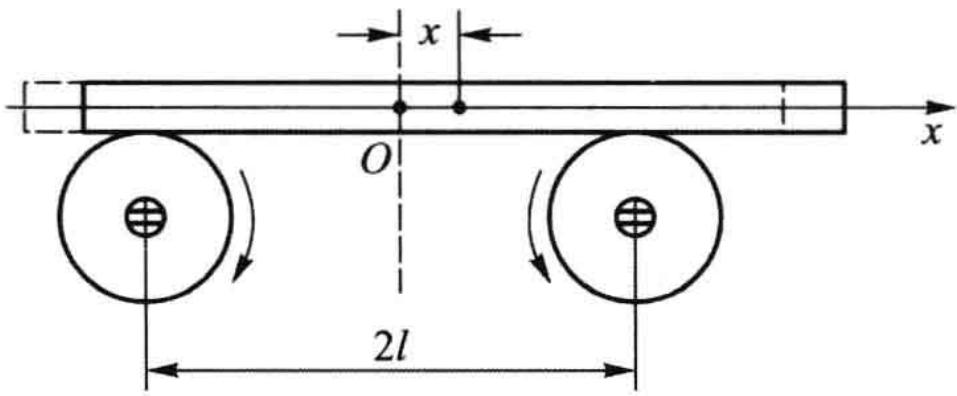
\includegraphics[width=0.4\textwidth]{figures/fig9-4_a.jpg}
  \end{figure}

\vfill
\newpage

\textbf{9-5.}一摆长为 $l$ , 摆锤质量为 $m$ 的单摆悬挂在火车顶上。当火车以加速度 $a_0$ 行驶时,

(1) 求证: 单摆平衡时, 摆线与竖直线之间将有一夹角 $\theta_{0}, \theta_{0}$ 的值为
$$
\theta_ {0} = \arctan \left(\frac {a _ {0}}{g}\right)
$$

(2) 将摆锤偏离平衡位置少许后释放, 求其振动周期。

\begin{figure}[H]
  \centering
  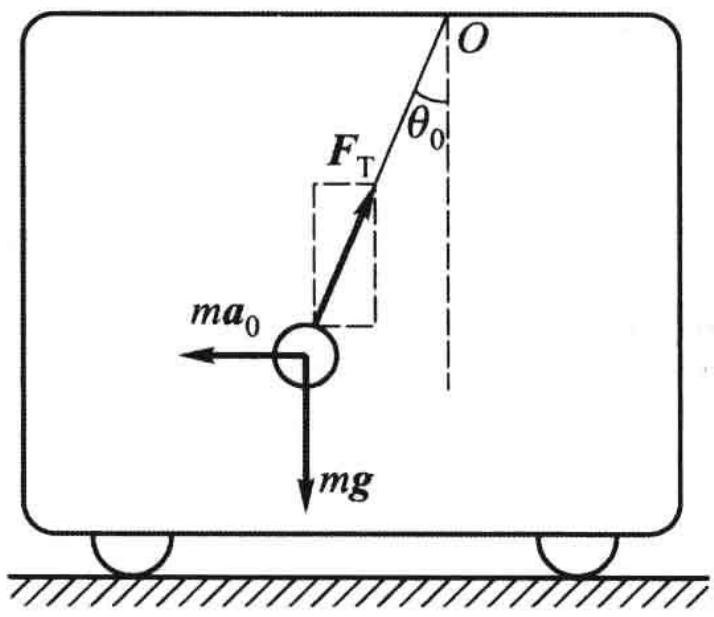
\includegraphics[width=0.25\textwidth]{figures/fig9-5.jpg}
  \end{figure}

\vfill

\textbf{9-6.}若上题中的单摆挂在电梯的顶上。

(1) 若电梯以加速度 $a_0$ 向下运动, 则摆的周期为多大? 若 $a_0 > g$ , 则会出现什么现象?

(2) 若电梯以加速度 $a_0$ 向上运动, 则摆的周期有多大?

\vfill
\newpage

\textbf{9-7.}由一长为 $l$ 、质量为 $m$ 的杆和一质量为 $m_0$ 、半径为 $R$ 的匀质圆盘组成的复摆，如习题9-7图所示。求此复摆在以下两种情况下的周期和等值单摆长。

(1) 圆盘与杆固连；

(2) 圆盘与杆之间由一光滑轴相连, 故圆盘可绕此轴自由旋转。

\begin{figure}[H]
  \centering
  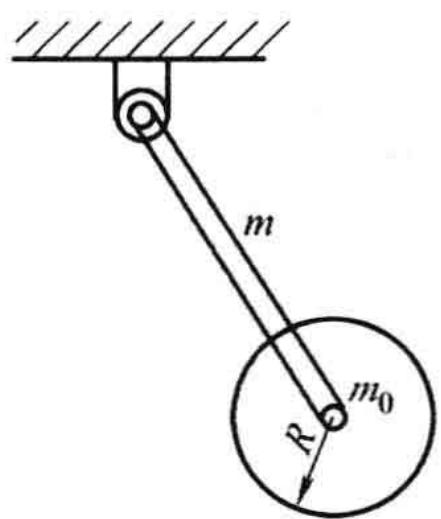
\includegraphics[width=0.25\textwidth]{figures/fig9-7.jpg}
  \end{figure}

\vfill

\textbf{9-8.}一半径为 $R$ 的光滑圆环以恒定的角速度 $\omega$ 绕其竖直的直径旋转, 圆环上套有一小珠。试求:

(1) 小珠相对圆环的平衡位置(以小珠与圆心连线同竖直直径间的夹角 $\theta_{0}$ 表示);

(2) 小珠在平衡位置附近做小振动的角频率。

\begin{figure}[H]
  \centering
  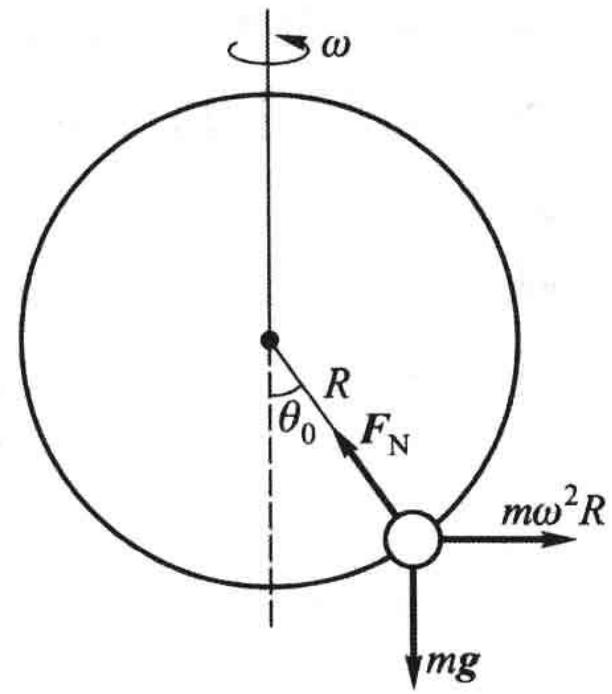
\includegraphics[width=0.25\textwidth]{figures/fig9-8.jpg}
  \end{figure}

\vfill
\newpage

\textbf{9-9.}如在质量均匀分布的球形行星上沿任一直径挖一隧道。将一物体由静止开始从一道口自由掉下。

(1) 求证物体到达隧道的另一道口所需的时间与物体的质量无关,与行星的直径无关,只与行星的密度 $\rho$ 有关,并计算该时间;

(2) 若隧道是沿行星的任一弦挖的, 求证该时间与弦的长短、位置均无关, 并证明该时间与(1)中的完全一样;

（3）若行星以角速度 $\omega_0\left(\omega_0 < \sqrt{\frac{4\pi\rho G}{3}}\right)$ 匀速自旋，角速度方向与隧道垂直，则(1)、(2)中的时间又为多大？

(4) 若上述行星为地球, 已知地球密度 $\rho_{0} = 5.52 \times 10^{3} \mathrm{~kg} / \mathrm{m}^{3}, G = 6.67 \times 10^{-11} \mathrm{~N} \cdot \mathrm{m}^{2} / \mathrm{kg}^{2}$ 。由于地球自旋角速度很小, 故可忽略。试计算 (1)、(2) 两问中所提及的时间。

\begin{figure}[H]
  \centering
  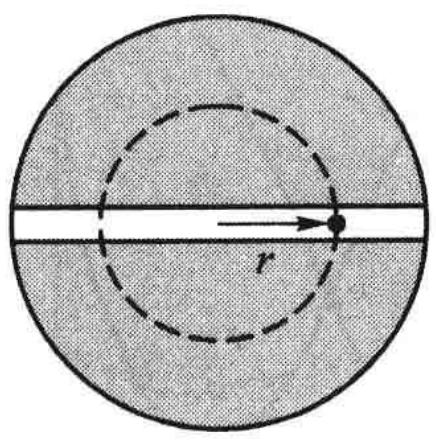
\includegraphics[width=0.2\textwidth]{figures/fig9-9.jpg}
  \end{figure}

\vfill

\textbf{9-10.}两个同方向同频率的简谐振动 $x_{1} = 0.4\cos \left(0.5\pi t + \frac{\pi}{6}\right)(\mathrm{m}), x_{2} = 0.2\cos (0.5\pi t + \varphi_{2})(\mathrm{m})$ ，试问：

(1) $\varphi_{2}$ 为何值时合振动的振幅最大？并求出此振幅值。

(2) 若合振动的初相位 $\varphi = \varphi_{2} + \frac{\pi}{2}$ ，则 $\varphi_{2}$ 为何值？

\vfill
\newpage

\textbf{9-11.}一架钢琴的“中音 C”有些不准,出于校准的需要,另取一架标准的钢琴,同时弹响这两架钢琴的“中音 C”键,在 1 分钟内听到 24 拍。试求待校准钢琴此键音的频率。

\vfill

\textbf{9-12.}两个互相垂直的振动表达式为:

$$
x = 3 \cos (2 \pi t), y = 3 \cos \left(4 \pi t + \frac {\pi}{3}\right)
$$

试作出合振动的轨迹图。

% \begin{figure}[H]
%   \centering
%   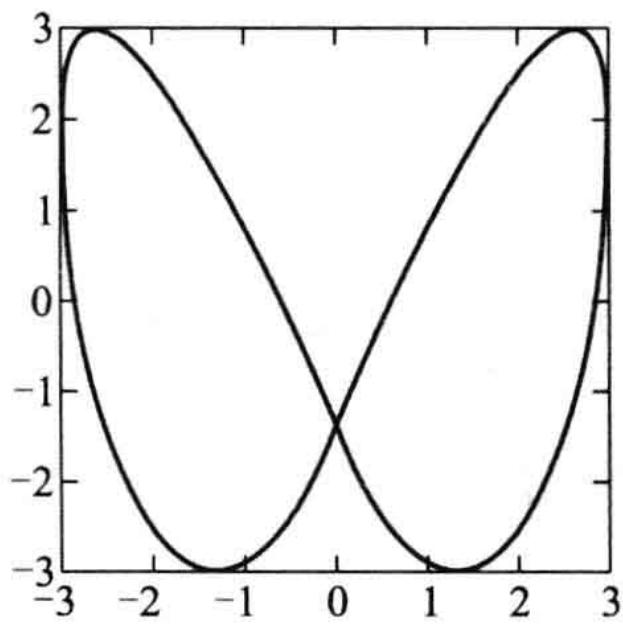
\includegraphics[width=0.4\textwidth]{figures/fig9-12.jpg}
%   \end{figure}

\vfill
\newpage


\textbf{9-13.}一根杆与竖直轴固连, 两者之间成 $\theta$ 角, 一根劲度系数为 $k$ , 原长为 $l_{0}$ 的弹簧套在杆上, 其一端与竖直轴相连, 另一端系一个同样套在杆上的质量为 $m$ 的小圆环,如习题9-13图所示。开始时杆以恒定的角速度 $\omega$ 绕竖直轴旋转,小圆环相对杆静止。

(1) 求此时小圆环的位置 $x_{0}$ ;

(2) 若转动角速度突然变为 $2 \omega$ , 则小圆环从位置 $x_{0}$ 运动到离轴最远处所需的时间 $t$ 为多大?

\begin{figure}[H]
  \centering
  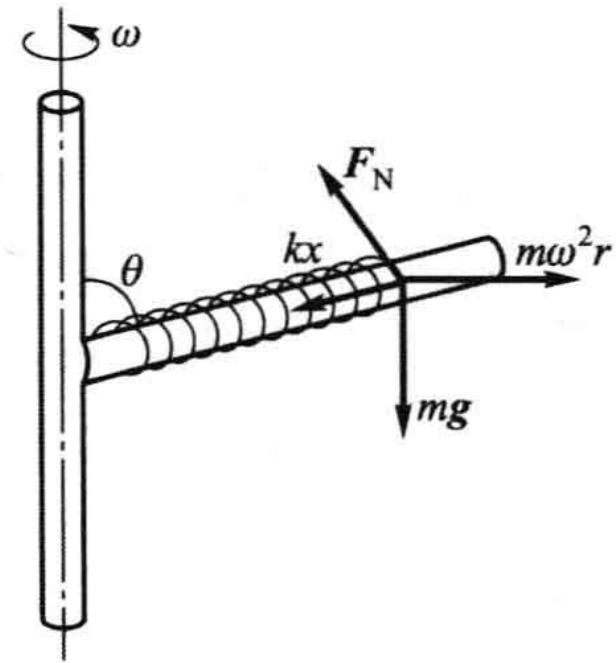
\includegraphics[width=0.25\textwidth]{figures/fig9-13.jpg}
  \end{figure}

\vfill

\textbf{9-14.}如习题 9-14 图所示, 在光滑的水平桌面上开有一小孔, 一条穿过小孔的细绳两头各系一质量分别为 $m_{1}$ 和 $m_{2}$ 的小球, 位于桌面上的小球 $m_{1}$ , 以 $v_{0}$ 的速度绕小孔做匀速圆周运动, 而小球 $m_{2}$ 则悬在空中, 保持静止。

(1) 求位于桌面部分的细绳的长度 $l_{0}$ ;

(2) 若给 $m_{1}$ 一微小的径向冲量, 则 $m_{2}$ 将做上下小振动, 求振动角频率 $\omega_{0}$ 。

\begin{figure}[H]
  \centering
  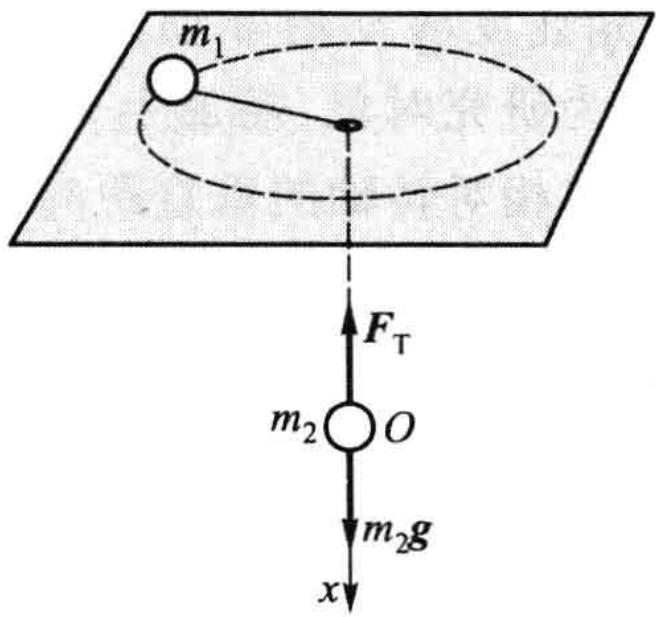
\includegraphics[width=0.25\textwidth]{figures/fig9-14.jpg}
  \end{figure}

\vfill
\newpage

\textbf{9-15.}一质量为 $m$ 、边长为 $a$ 的正三角形薄板, 通过其某一角悬挂在与板面垂直的光滑水平轴上, 构成一复摆。求此复摆的周期和等值单摆长。

\begin{figure}[H]
  \centering
  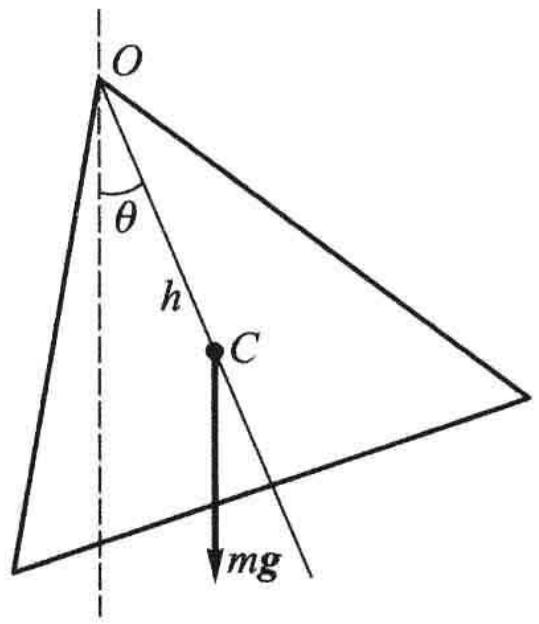
\includegraphics[width=0.2\textwidth]{figures/fig9-15_a.jpg}
  \end{figure}

\vfill

\textbf{9-16.}质量为 $m_{0}$ 的小球和长为 $l$ 、质量为 $m$ 的杆组成的复摆, 被刚性地固定在一横轴上, 而横轴被架在一平台上的两个支架上, 如习题 9-16 图所示。当平台以较小的角速度 $\Omega$ 绕其中心轴(通过摆的上端)旋转时,求该复摆的振动周期,设小球的半径可忽略。

\begin{figure}[H]
  \centering
  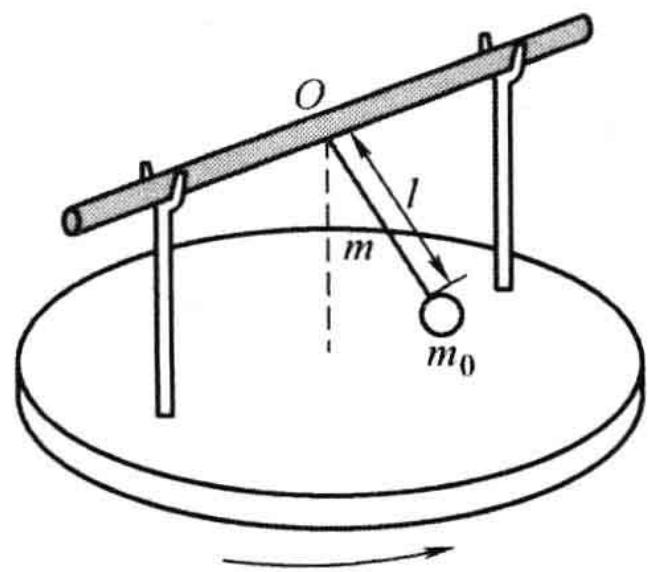
\includegraphics[width=0.2\textwidth]{figures/fig9-16.jpg}
  \end{figure}

\vfill
\newpage

\textbf{9-17.}如习题 9- 17 图所示,一深水池中竖立着一根光滑的细杆,一长度为 $L$ 的匀质细管套在杆上。用手持管,使其下端正好与水面接触,然后放手,设水的密度为 $\rho_{0}$ 。

(1) 若管运动到最低位置时, 其上端正好与水面持平, 求管的密度 $\rho_{1}$ ;

(2) 证明在(1)中情况下,细管将做简谐振动,求出振幅和周期;

(3) 若管的密度为 $\frac{4}{3} \rho_{1}$ , 求管下沉到最低位置所需的时间。

\begin{figure}[H]
  \centering
  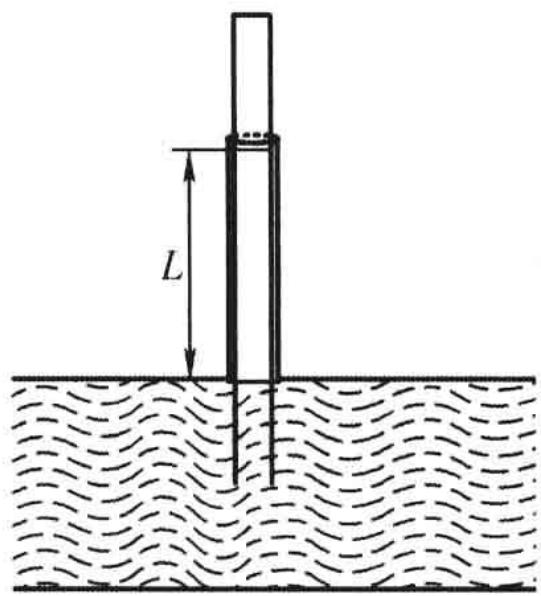
\includegraphics[width=0.25\textwidth]{figures/fig9-17.jpg}
  \end{figure}

\vfill

\textbf{9-18.}试作出下列两振动的合振动的李萨如图：

(1) $x = \cos \omega t, y = \cos 2\omega t$ 。

(2) $x = \cos 2\omega t, y = \cos (3\omega t + \pi)$ 。

% \begin{figure}[H]
%   \centering
%   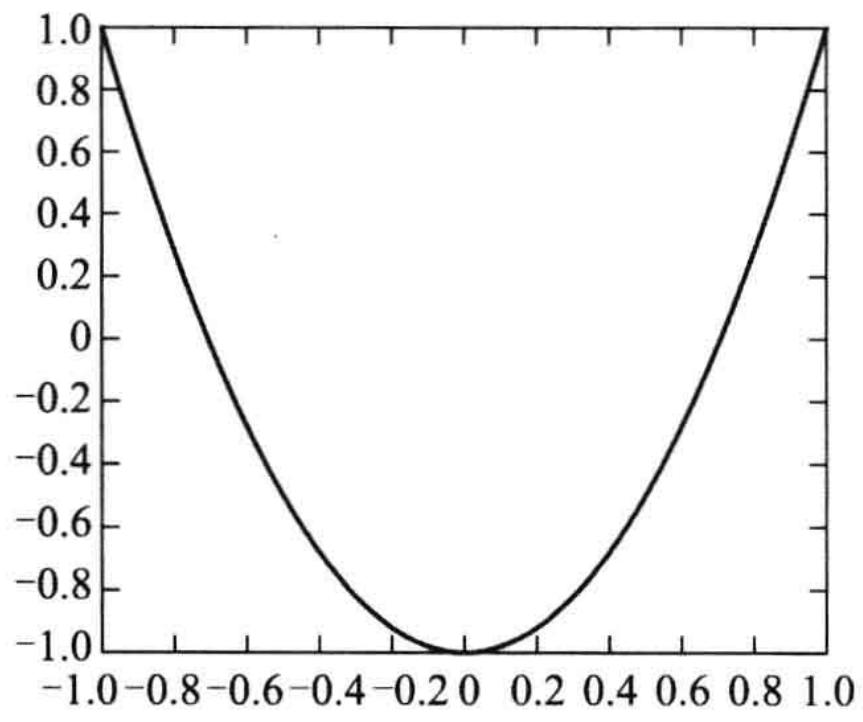
\includegraphics[width=0.4\textwidth]{figures/fig9-18_a.jpg}
%   \end{figure}

\vfill
\newpage

\textbf{9-19.}一质量为 $m_{0}$ 的物块置于一光滑水平面上, 物块的两端各系有一弹簧, 弹簧的自然长度均为 20 cm, 其劲度系数分别为 $k_{1}$ 与 $k_{2}$ 。现将两弹簧分别与两壁相连, 两壁与两弹簧原来的自由端都相距 10 cm, 如习题 9-19 图所示。设 $k_{1}=1\ N/m, k_{2}=3\ N/m, m_{0}=100\ g$ 。

(1) 当物块处于平衡位置时, 求每个弹簧的长度;

(2) 若将此物块略微偏离平衡位置后释放,试求其振动周期;

(3) 设此物块振动的振幅为 $5 \mathrm{~cm}$ , 当其通过平衡位置时, 有一质量为 $m = 100 \mathrm{~g}$ 的泥灰竖直地落于其上, 并与之一起运动, 试求此系统的振动周期和振幅;

(4) 若(3)中的泥灰在物块运动到最大位移处时落于其上,求这种情况下系统振动的周期和振幅。

\begin{figure}[H]
  \centering
  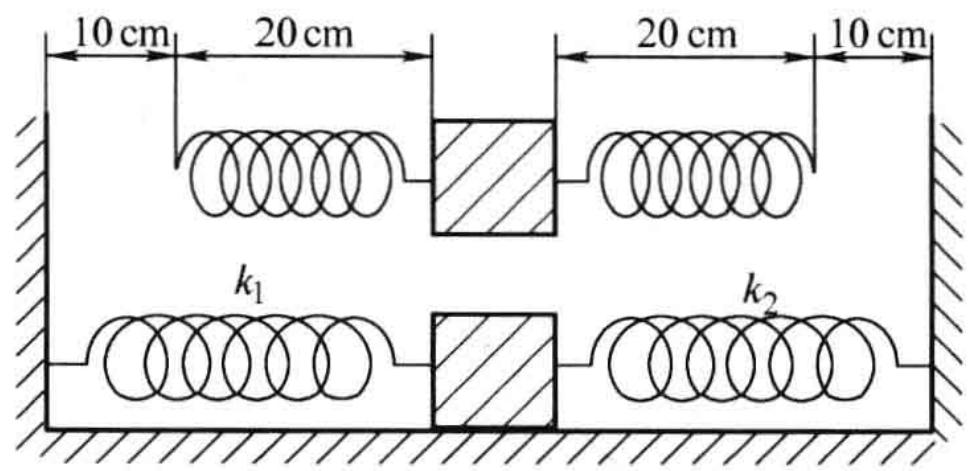
\includegraphics[width=0.3\textwidth]{figures/fig9-19_2.jpg}
  \end{figure}

\vfill

\textbf{9-20.}如习题 9-20 图所示, 一弹簧振子, 其质量 $m_{1} = 98 \mathrm{~g}$ , 劲度系数 $k_{1} = 9.8 \times 10^{-2} \text{ N/cm}$ , 它的影子水平地投射到一质量 $m_{2} = 980 \text{ g}$ 的屏上, 屏在一劲度系数 $k_{2} = 0.98 \text{ N/cm}$ 的弹簧下。开始时把两者都从平衡位置拉下 $10 \text{ cm}$ , 先释放弹簧振子使之振动。如果要使影子在屏上振动的振幅为 $5 \text{ cm}$ , 试问应隔几秒钟后释放屏使之振动? 并写出此时影子在屏上的振动方程。

\begin{figure}[H]
  \centering
  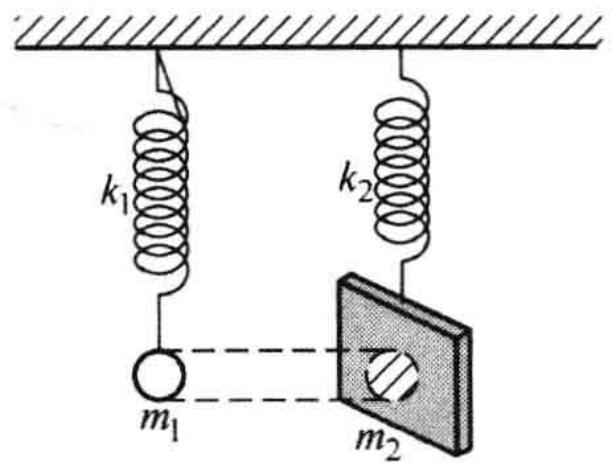
\includegraphics[width=0.3\textwidth]{figures/fig9-20.jpg}
  \end{figure}

\vfill
\newpage

\textbf{9-21.}一面积为 $S$ 、质量为 $m$ 的薄板连在弹簧的下端, 弹簧的上端固定, 薄板浸在黏性液体中,如习题9-21图所示。设薄板在黏性液体中受到的阻力 $F_{f}=-2\mu Sv$ ,式中v为薄板在竖直方向上的运动速度, $\mu$ 是一个与液体黏性有关的常量。设此系统的振动周期为T,求此系统在空气中时的振动周期 $T_{0}$ 。

\begin{figure}[H]
  \centering
  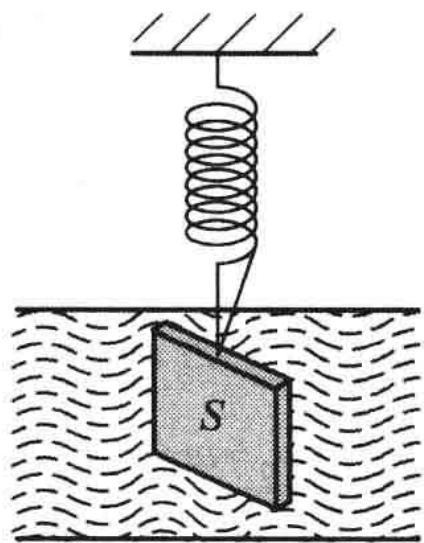
\includegraphics[width=0.25\textwidth]{figures/fig9-21.jpg}
  \end{figure}

\vfill

\textbf{9-22.}一质量为 $0.2 \mathrm{~kg}$ 的物体, 悬于颈度系数为 $10 \mathrm{~N} / \mathrm{m}$ 的弹簧下, 此物体受到的阻力 $F_{\mathrm{f}} = -b v$ , 其中 $v$ 是物体的速度 (单位是 $\mathrm{m} / \mathrm{s}$ ), $b$ 为一较小的常量。

(1) 写出系统振动的运动方程;

(2) 若系统振动频率比无阻尼时小了万分之一, 即 $\frac{\omega_0 - \omega_f}{\omega_0} = 10^{-4}$ , 则常量 $b$ 为多大?

(3) 此系统的 $Q$ 值为多大? 振动经一个整周期后, 振幅减弱为几分之几?

\vfill
\newpage

\textbf{9-23.}某阻尼振动的振幅在一个周期后减为原来的 $1 / 4$ , 问此振动周期比无阻尼存在时的周期大百分之几?

\vfill

\textbf{9-24.}一摆长为 $l = 0.750 \mathrm{~m}$ 的单摆做阻尼振动, 经过一分钟后, 其振幅衰减为开始时的 $1 / 8$ , 求对数减缩 $\lambda$ (即 $\lambda = \delta T$ )。

\vfill
\newpage

\textbf{9-25.}某振动系统从开始振动,经过16次振动后,能量减为开始时的0.6。问再经过16次振动后,系统能量减为开始时的几分之几?

\vfill

\textbf{9-26.}当在某钢琴上弹响“中音 C”这个琴键时, 其振动能量在 $1 \mathrm{~s}$ 内减至初始值的一半。已知中音 C 的频率为 $256 \mathrm{~Hz}$ 。求此系统的 Q 值。

\vfill
\newpage

\textbf{9-27.}一质量为 $10 \mathrm{~kg}$ 的物体, 从 $0.5 \mathrm{~m}$ 高处静止下落到弹簧秤的秤盘里, 并黏附在盘上。已知秤盘的质量为 $2.0 \mathrm{~kg}$ , 弹簧的劲度系数为 $980 \mathrm{~N} / \mathrm{m}$ 。为使秤盘在最短时间内停下来, 就须附上一阻尼系统。求出所必需的阻尼因数 $\delta$ , 并写出秤盘的位置 $y$ 随时间 $t$ 的变化关系 ( $y$ 的零点取在平衡位置, $t$ 的零点取在物体掉在秤盘的瞬间)。

\vfill

\textbf{9-28.}摆长为 $1 \mathrm{~m}$ 的单摆, 在振动 50 次后振幅减为原来的 $\frac{1}{\mathrm{e}}$ 。现使其悬点做振幅为 $1 \mathrm{~mm}$ 的水平方向上的简谐振动。

(1) 若摆锤的水平位移为 $x_{1}$ , 悬点的水平位移为 $x_{2}$ , 试证明摆锤做微小振动时的运动方程为 $\frac{\mathrm{d}^{2} x_{1}}{\mathrm{d} t^{2}} + 2 \delta \frac{\mathrm{d} x_{1}}{\mathrm{d} t} + \frac{g}{l} x_{1} = \frac{g}{l} x_{2}$ 。如果 $x_{2} = A \cos \omega t$ , 试求此方程的稳态解。

(2) 求共振时摆锤运动的振幅。

(3) 在什么角频率时, 其振幅为共振时的一半?

\begin{figure}[H]
  \centering
  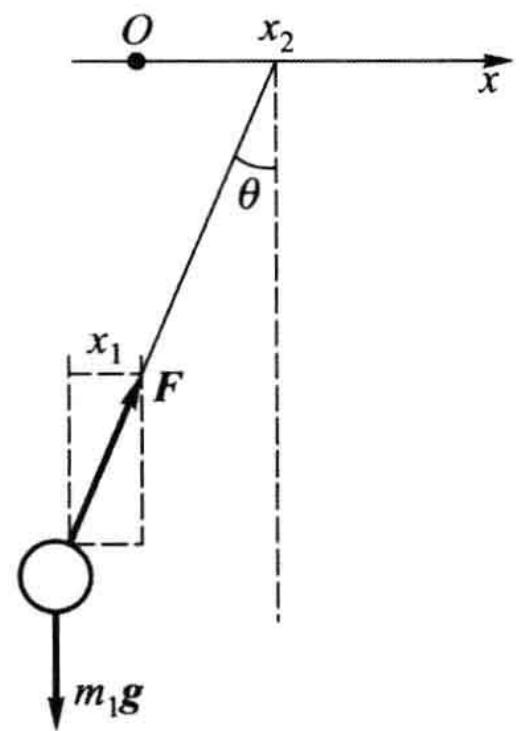
\includegraphics[width=0.23\textwidth]{figures/fig9-28.jpg}
  \end{figure}

\vfill
\newpage

\textbf{9-29.}一谐振子质量 $m = 0.10 \mathrm{~kg}$ , 做周期 $T = 2.5 \mathrm{~s}$ 的简谐振动, 质点振动的总能量 $E = 0.20 \mathrm{~J}$ , 求作用在质点上力的最大值。

\vfill

\textbf{9-30.}一物体悬挂于弹簧下,系统固有振动周期为 $0.50 \mathrm{~s}$ ,今在物体上加一竖直方向的余弦力,其最大值 $F = 1 \times 10^{-3} \mathrm{~N}$ ;此外物体还受到一摩擦阻力 $F_{\mathrm{f}} = -C \dot{x}$ 作用, $C$ 为一较小的常量。已知系统在共振时的振幅为 $5.0 \mathrm{~cm}$ ,求物体在运动过程中受到的最大摩擦力的数值 $F_{\mathrm{f,max}}$ 。

\vfill
\newpage

\textbf{9-31.}做受迫振动的振子, 若其速度与强迫力同相位, 求强迫力的频率。设振子的固有频率为 $\omega_{0}$ 。

\vfill

\textbf{9-32.}一振子在强迫力 $F = F_{0} \cos \omega t$ 的驱动下做受迫振动。已知振子的质量 $m = 0.2 \mathrm{~kg}$ ，弹簧的劲度系数 $k = 80 \mathrm{~N} / \mathrm{m}$ ，阻力系数 $C = 4 \mathrm{~N} \cdot \mathrm{s} / \mathrm{m}$ ，若 $F_{0} = 2 \mathrm{~N}$ ， $\omega = 30 \mathrm{~s}^{-1}$ 。试问：

(1) 振子系统在一周内反抗阻力而耗散的能量是多少?

(2) 输入系统的平均功率是多少?

\vfill
\newpage

\textbf{9-33.}某振动系统的固有频率为 $1000 \mathrm{~Hz}$ , 品质因数为 50, 若其共振时驱动力所提供的平均功率为 $5.0 \mathrm{~mW}$ , 求此时振子的能量。

\vfill

\textbf{9-34.}习题 9-34 图所示为某振动系统在驱动力 $F = F_{0} \sin \omega t$ 的驱动下的平均功率共振曲线。此处 $F_{0}$ 是常量。

(1) 求出此系统的固有频率 $\omega_{0}$ 和品质因数 Q 的数值；

(2) 若撤去驱动力, 则系统经过多少周后能量降至初始值的 $e^{-5}$ ?

\begin{figure}[H]
  \centering
  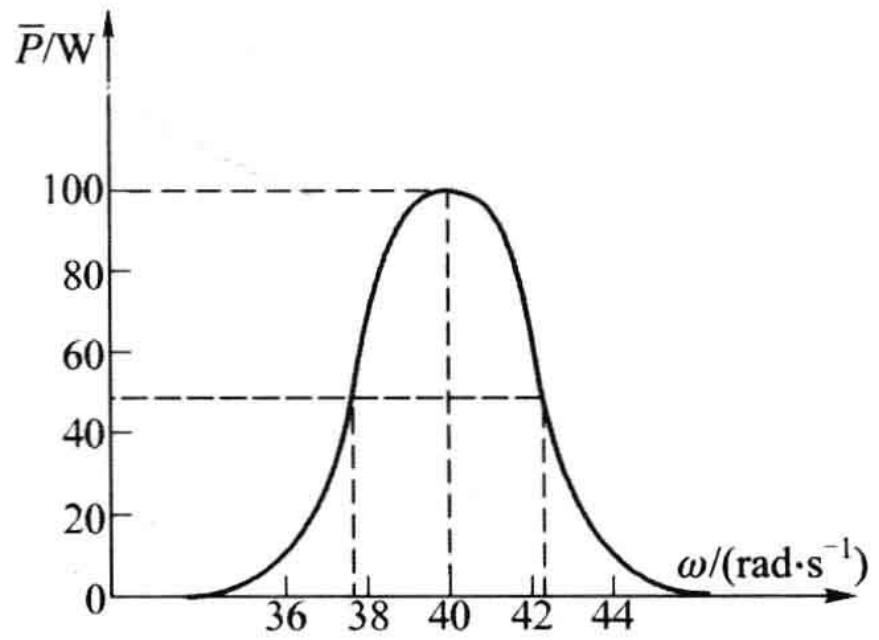
\includegraphics[width=0.4\textwidth]{figures/fig9-34.jpg}
  \end{figure}

\vfill
\newpage

\textbf{9-35.}两个质量都为 $m$ 的质点, 如习题 9-35 图连接在三个劲度系数都是 $k$ 的弹簧上, 两质点间连接一质量可以忽略的阻尼减震器, 阻尼减震器所施的力为 $bv$ , 这里 $v$ 是它两端的相对速度, $b$ 为常量。该力阻止其两端之间 (即两质点之间) 的相对运动。令 $x_{1}, x_{2}$ 分别为两质点离开其平衡位置的位移。

(1) 写出每个质点的运动方程；

(2) 证明运动方程可以用新的变量 $y_{1} = x_{1} + x_{2}$ 和 $y_{2} = x_{1} - x_{2}$ 来求解；

(3) 证明: 如果两质点原来静止于平衡位置, 在 $t = 0$ 时给质点 1 以初速度 $v_{0}$ , 则在足够长的时间以后, 两个质点的运动方程为 $x_{1} = x_{2} = \frac{v_{0}}{2 \omega} \sin \omega t$ , 并求出 $\omega$ 。

\begin{figure}[H]
  \centering
  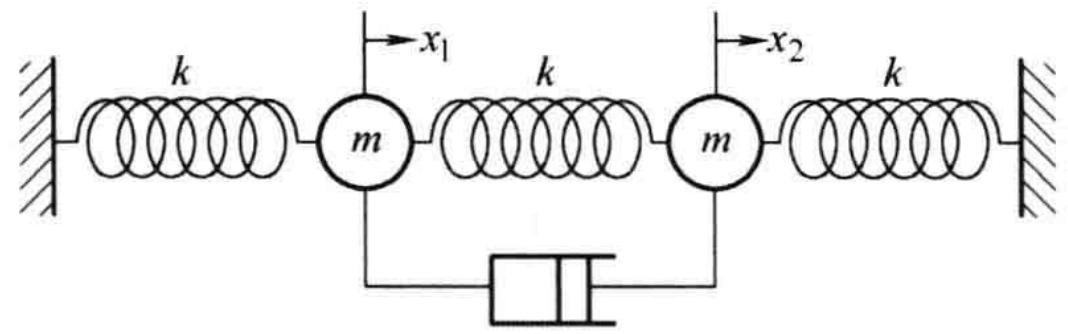
\includegraphics[width=0.4\textwidth]{figures/fig9-35_1.jpg}
  \end{figure}

\vfill

\textbf{9-36.}由劲度系数为 $k$ 的轻弹簧和质量为 $m$ 的质点构成的两个相同弹簧振子串联地竖直悬挂, 求此系统沿竖直方向做振动的简正频率。

\begin{figure}[H]
  \centering
  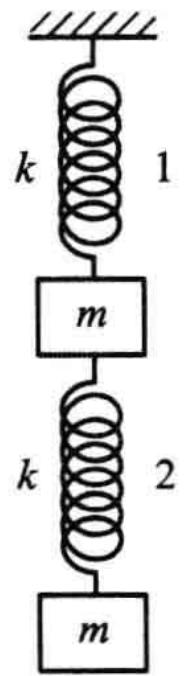
\includegraphics[width=0.08\textwidth]{figures/fig9-36.jpg}
\end{figure}

\vfill
\newpage


\textbf{10-1.}人耳能听到的声音频率范围一般为 $20 \sim 20000 \mathrm{~Hz}$ 。试计算在 $25^{\circ} \mathrm{C}$ 的海水中人耳能听到的声音的波长范围。已知声音在 $25^{\circ} \mathrm{C}$ 海水中的传播速度为 $1531 \mathrm{~m} / \mathrm{s}$ 。

\vfill

\textbf{10-2.}由海底的地震所激发的潮浪, 称为海啸。由于大洋的平均深度大约是 $5 \mathrm{~km}$ , 而潮浪的水平长度大于 $5 \mathrm{~km}$ , 故可认为是一种浅水波。若海底地震的震中与海岸的距离为 $100 \mathrm{~km}$ , 试估算潮浪传到海岸所需的时间。

\vfill
\newpage

\textbf{10-3.}设有一简谐横波 $y = 5.0 \cos \left[2\pi \left(\frac{t}{0.05} - \frac{x}{10}\right)\right]$ ，其中 $x, y$ 的单位为 $\mathrm{cm}, t$ 的单位为 $\mathbf{s}$ 。试求：

(1) 振幅 A、频率 v、波长 $\lambda$ 以及波速 v；

(2) 若某处振动的初相位为 $\frac{3}{5}\pi$ ，求该处的位置 x。

\vfill

\textbf{10-4.}一根质量线密度为 $4 \times 10^{-3} \mathrm{~kg} / \mathrm{m}$ 的均匀钢丝, 被 $10 \mathrm{~N}$ 的力所拉紧。钢丝的一端有一正弦式的横向波扰动, 经过 $0.1 \mathrm{~s}$ , 此波扰动即传到钢丝的另一端, 而扰动源正好经历 100 个周期。求波长。

\vfill
\newpage

\textbf{10-5.}一正弦横波沿一弦线自左向右传播,传播速度为 $80 \mathrm{~cm} / \mathrm{s}$ 。观察弦上某点的运动,发现该点在做振幅为 $2 \mathrm{~cm}$ 、频率为 $10 \mathrm{~Hz}$ 的简谐振动。若取该点为坐标 $x$ 的原点,当 $t = 0$ 时,该点正好位于原点,且具有向 $y$ 轴正方向运动的速度。试求:

(1) 此波的波长 $\lambda$ ;

(2) 弦上该点的振动方程;

(3) 此波的运动学方程;

(4) 弦上 $x = 4 \mathrm{~cm}$ 处质点振动的初相位 $\varphi'$ 。

\vfill

\textbf{10-6.}设入射波的方程为 $y = 0.2\cos (\pi t - 1.5\pi x + 0.4\pi)$ ，其中 $x, y$ 的单位是 $m, t$ 的单位是 $s$ 。波在 $x = 0$ 处反射。试就以下两种情况，求在振幅不衰减情况下合成驻波的方程，并指出 $x = 0$ 处是波节还是波腹。

(1) x=0 处是自由端；

(2) x=0 处是固定端。

\vfill
\newpage

\textbf{10-7.}两根完全相同的琴弦, 它们的基频都是 $357 \mathrm{~Hz}$ 。其中一根琴弦的弦轴略有松动, 以致该弦的张力以恒定的速率减小, 其每秒减小量 $\Delta F_{\mathrm{T}}$ 与原张力 $F_{\mathrm{T} 0}$ 之比为 0.001 。问经过多少时间, 此两琴弦同时发声时会产生 $1 \mathrm{~Hz}$ 的拍频?

\vfill

\textbf{10-8.}一装置于海底的超声波探测器, 发出一束频率为 $30000 \mathrm{~Hz}$ 的超声波, 被向着探测器驶来的潜艇反射回来, 反射波与原来的波合成后, 得到频率为 $241 \mathrm{~Hz}$ 的拍。求潜艇的速率。设超声波在海水中的波速为 $1500 \mathrm{~m} / \mathrm{s}$ 。

\vfill
\newpage

\textbf{10-9.}一平面简谐波沿 $x$ 轴方向传播, 其表示式为
$$
y = A \cos (\omega t - k x + \varphi_ {0})
$$
在 $x=x_{0}$ 固定端处反射。求反射波的表示式，振幅不衰减。

\vfill

\textbf{10-10.}在绳索上传播的波, 其表示式为 $y = 3\cos \left[2\pi \left(\frac{t}{0.1} - \frac{x}{10}\right) - \frac{\pi}{3}\right]$ , 式中 $x, y$ 的单位为 $\mathrm{cm}, t$ 的单位为 $\mathrm{s}$ 。为在绳索上形成驻波 (在 $x = 0$ 处为波节), 则应叠加一个什么样的波? 写出此波的表示式。并写出驻波的表示式。

\vfill
\newpage


\textbf{10-11.}一波沿 $x$ 轴传播, 观察到 $x$ 轴上两点 $x_{1}$ 和 $x_{2}$ 处介质的质点均做频率为 $2.0 \mathrm{~Hz}$ 的简谐振动, $x_{1}$ 处振动相位比 $x_{2}$ 处落后 $\frac{\pi}{4}$ 。已知 $x_{2} - x_{1} = 3.0 \mathrm{~cm}$ 。

(1) 试问此波是沿正 x 轴方向传播, 还是沿负 x 轴方向传播? (设 $\lambda > 6 \, cm$ )

(2) 试求波长 $\lambda$ 和波速 v。

\vfill

\textbf{10-12.}在拉紧的弦上传播的一个波脉冲可表示为
$$
y (x, t) = \frac {b ^ {3}}{b ^ {2} + (2 x - u t) ^ {2}}
$$
式中 b、u 均为常量。

(1) 画出 t=0 时的波形图。

(2) 波脉冲传播的速率及方向如何?

(3) 试求 $t = 0$ 时刻弦上任一点 $x$ 的横向速度。


\vfill
\newpage

\textbf{10-13.}入射波在固定端全反射,某一瞬时的波形如习题 10- 13 图(a)所示。试画出此瞬时反射波的波形图。

\begin{figure}[H]
  \centering
  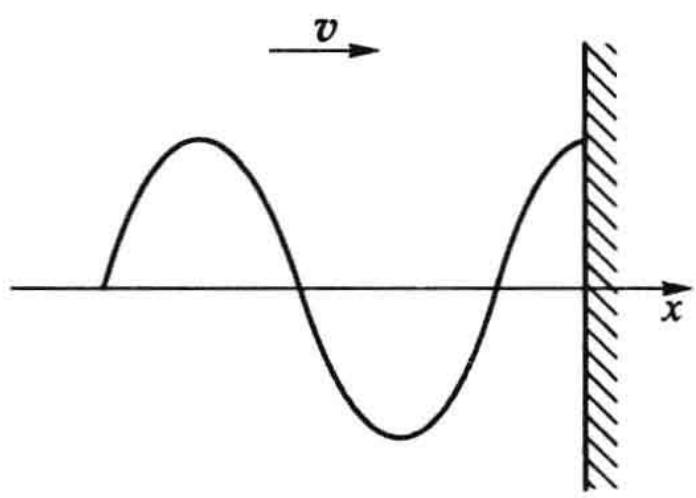
\includegraphics[width=0.3\textwidth]{figures/fig10-13_b.jpg}
  \end{figure}

\vfill

\textbf{10-14.}如习题 10-14 图所示, 一根线密度为 $0.15 \mathrm{~g} / \mathrm{cm}$ 的弦线, 其一端与一频率为 $50 \mathrm{~Hz}$ 的音叉相连, 另一端跨过一定滑轮后悬一重物给弦线提供张力, 重物质量为 $m$ , 音叉到滑轮间的距离为 $1 \mathrm{~m}$ . 当音叉振动时, 为使弦上形成一个、两个、三个波腹, 则重物的质量 $m$ 应各为多大?

\begin{figure}[H]
  \centering
  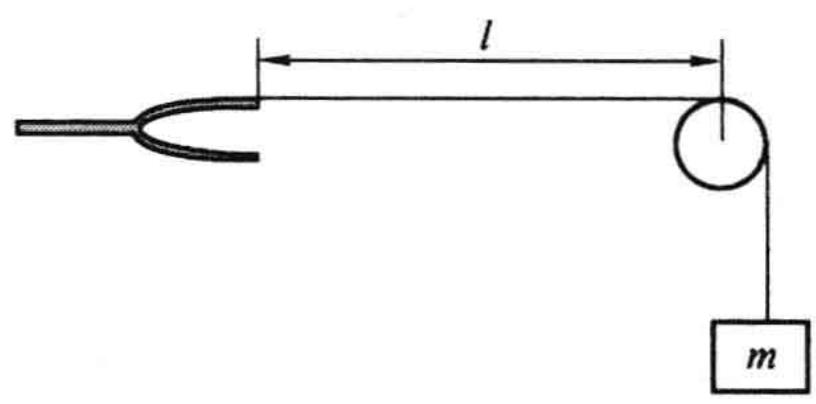
\includegraphics[width=0.35\textwidth]{figures/fig10-14.jpg}
  \end{figure}

\vfill
\newpage

\textbf{10-15.}在一半径为 $10 \mathrm{~cm}$ 的圆柱形管子里, 一平面简谐空气波沿轴向传播, 波长和频率分别为 $\lambda = 80 \mathrm{~cm}, \nu = 425 \mathrm{~Hz}$ , 波的能流密度为 $1.7 \times 10^{-2} \mathrm{~J} / (\mathrm{~s} \cdot \mathrm{m}^{2})$ 。试求:

(1) 管中波的平均能量密度和最大能量密度;

(2) 每两个相邻同相位面间的总能量。

\vfill

\textbf{10-16.}一波源以 $35000 \mathrm{~W}$ 的功率发射球面电磁波。在某处测得该波的平均能量密度为 $7.8 \times 10^{-15} \mathrm{~J} / \mathrm{m}^{3}$ 。求该处离波源的距离。电磁波的传播速度为 $3.0 \times 10^{8} \mathrm{~m} / \mathrm{s}$ 。

\vfill
\newpage

\textbf{10-17.}以下两列波在介质中叠加：
$$
y _ {1} = A \cos (6 t - 5 x), y _ {2} = A \cos (5 t - 4 x)
$$
(式中 $x, y_{1}, y_{2}$ 的单位是 m, t 的单位是 s)

(1) 求此两列波的相速度 $v_{p1}$ 、 $v_{p2}$ ;

(2) 写出合成波的方程, 并求出振幅为零的相邻两点之间的距离;

(3) 求群速度 $v_{g}$ 。

\vfill

\textbf{10-18.}水上短波长 $(\lambda \leqslant 1 \mathrm{~cm})$ 的涟波运动, 是受表面张力控制的。这种涟波的相速度为 $v_{\mathrm{p}} = \left(\frac{2 \pi \sigma}{\rho \lambda}\right)^{\frac{1}{2}}$ , 式中 $\sigma$ 为表面张力系数, $\rho$ 为水的密度。

(1) 证明:由接近某给定波长 $\lambda$ 的诸波长所构成的扰动,群速度等于 $\frac{3}{2}v_{p}$ ;

(2) 若波群只有两个波组成, 此两波的波长分别为 $0.99 \mathrm{~cm}$ 和 $1.01 \mathrm{~cm}$ , 则波群两相邻峰值间的距离为多大?

\vfill
\newpage

\textbf{10-19.}对于深水波,考虑到表面张力,其色散关系为 $\omega^2 = g k + \frac{\sigma k^3}{\rho}$ ,式中水的密度 $\rho = 1.0 \times 10^{3} \mathrm{~kg} / \mathrm{m}^{3}$ , 表面张力 $\sigma = 7.2 \times 10^{-2} \mathrm{~N} / \mathrm{m}$ 。

(1) 求出相速度和群速度与 k 的函数关系;

(2) 证明对于波长接近 $1.7 \times 10^{-2} \mathrm{~m}$ 的诸波所构成的水波, 其相速度与群速度相等, 并求出速度值。

\vfill

\textbf{10-20.}把两根连在一起的弦线拉紧,设想有一行波入射到相接处,为使反射波的振幅 $B$ 与入射波的振幅 $A$ 之比 $\frac{B}{A} = \frac{1}{3}$ 。试求:

(1) 两根弦线的线密度之比 $\eta_{1}: \eta_{2}$ , 设入射波从弦线 1 向弦线 2 方向传播;

(2) 透射波的振幅 C 与入射波振幅 A 之比 $\frac{C}{A}$ 。

\vfill
\newpage

\textbf{10-21.}一列纵波在两种介质的界面上发生反射。设入射波与反射波的振动方向不变, 在入射波所在的介质中纵波的波速是横波波速的 $\sqrt{3}$ 倍。试问为使反射波是一横波, 则入射角应为多大?

\begin{figure}[H]
  \centering
  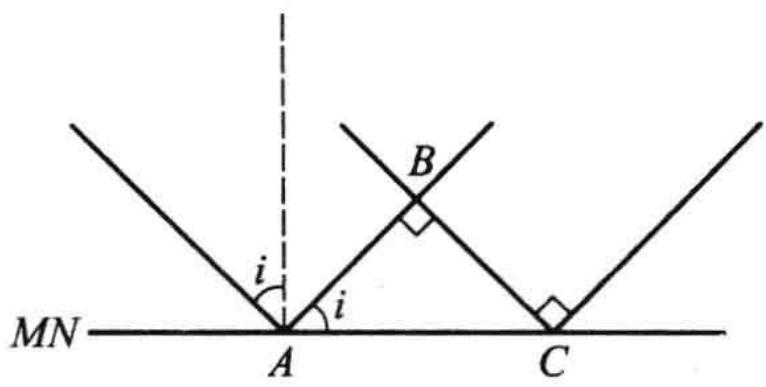
\includegraphics[width=0.4\textwidth]{figures/fig10-21.jpg}
\end{figure}

\vfill
\newpage

\textbf{11-1.} S'系相对 S 系以速度 $v = 0.8c$ 沿 $x$ 轴运动。S'系和 S 系的原点在 $t = t' = 0$ 时重合。一事件在 S'系中发生在 $x' = 300 \mathrm{~m} (y' = z' = 0)$ , $t' = 2 \times 10^{-7} \mathrm{~s}$ 。求该事件在 S 系中发生的空间位置 $x$ 和时间 $t$ 。

\vfill

\textbf{11-2.}在一惯性系的同一地点,先后发生两个事件,其时间间隔为 $0.2 \mathrm{~s}$ , 而在另一惯性系中测得此两事件的时间间隔为 $0.3 \mathrm{~s}$ , 求两惯性系之间的相对运动速率。

\vfill
\newpage

\textbf{11-3.}S'系相对 S 系以恒定速度沿 x 轴运动。在 S 系中两事件发生在同一时刻, 并沿 x 轴相距 $2 \times 10^{4}$ m。而在 S'系中, 测得两事件的空间间隔为 $3 \times 10^{4}$ m, 试问在 S'系中测得的两事件的时间间隔是多少?

\vfill

\textbf{11-4.}一火箭飞船经地球飞往某空间站,该空间站相对地球静止,与地球之间的距离为 $9.0 \times 10^{9} \mathrm{~m}$ 。地球上的钟和空间站上的钟是同步校准的。当火箭飞船飞经地球时,宇航员将飞船上的钟拨到与地球上的钟相同的示数。当火箭飞船飞经空间站时,宇航员发现飞船上的钟比空间站上的钟慢了 $3 \mathrm{~s}$ 。求火箭飞船的飞行速率。

\vfill
\newpage

\textbf{11-5.}一飞船以 $v = 0.6c$ 的速率沿平行于地面的轨道飞行。飞船上沿运动方向放置一根杆子，在地面上的人测得此杆子的长度为 $l$ ，求此杆子的本征长度 $l_{0}$ 。

\vfill

\textbf{11-6.}一道闪光从 $O$ 点发出, 在 $P$ 点被吸收。在 S 系中, $OP$ 具有长度 $l$ 且

同 x 轴成 $\theta$ 角, 如习题 11-6 图所示。在相对于 S 系以恒速 v 沿 x 轴运动的 S' 系中:

(1) 从光的发出到吸收相隔多长时间 $\Delta t'$ ?

(2) 光的发出点 O 到吸收点 P 的空间间隔 $l'$ 是多大?

\vfill
\newpage

\textbf{11-16.}两根相互平行的米尺,各以 $v = \frac{3}{5} c$ 的速率相向运动,运动方向平行于尺子。求任一尺子上的观察者测量另一尺子的长度。

\vfill


\textbf{11-17.}静长为 $L$ 的车厢, 以恒定速率 $v$ 沿地面向右运动。自车厢的左端 $A$ 点发出一光信号, 经右端 $B$ 点镜面反射后回到 $A$ 端。

(1) 在车厢里的人看来, 光信号经多少时间 $\Delta t_{1}^{\prime}$ 到达 $B$ 端? 从 $A$ 发出经 $B$ 反射后回至 $A$ , 共需多少时间 $\Delta t^{\prime}$ ?

(2) 在地面上的人看来, 光信号经多少时间 $\Delta t_{1}$ 到达 $B$ 端? 从 $A$ 发出经 $B$ 反射后回至 $A$ , 共需多少时间 $\Delta t$ ?

\vfill\newpage

\textbf{11-18.}一艘静长为 $90 \mathrm{~m}$ 的飞船以速度 $v = 0.8 c$ 飞行。当飞船的尾部经过地面上某信号站时, 该信号站发出一光信号。

(1) 当光信号到达飞船头部时, 飞船头部离地面信号站的距离为多远?

(2) 按地面上的时间, 信号从信号站发出共需多少时间 $\Delta t$ 才能到达飞船头部?

\vfill


\textbf{11-19.}三艘飞船 A、B、C 沿同一直线飞行。B 船上的观察者发现，A、C 两船以 $v = 0.7c$ 的相同速率远离 B 船。

(1) 求 A 船上的观察者观测到的 B、C 两船的速率；

(2) 若 B 船相对地面的飞行速率为 $v_{\mathrm{B}} = 0.9c$ , 求 A、C 两船相对地面的飞行速率。

\vfill\newpage

\textbf{11-20.}在实验室里测得一根沿 $x$ 方向运动的棒与 $x$ 轴的夹角 $\theta_{1} = 45^{\circ}$ 。在相对实验室参考系以 $v = 0.6c$ 的速度沿 $x$ 方向运动的另一参考系 $\mathbf{S}'$ 系中, 测得此夹角 $\theta' = 35^{\circ}$ 。

(1) 求棒相对实验室参考系的运动速度；

(2) 棒相对 S' 系的运动速度为多大?

(3) 在棒静止的参考系 S" 中, 棒与 x" 轴的夹角 $\theta'$ 为多大?

\vfill


\textbf{11-21.}一航天飞机沿 $x$ 方向飞行, 接静止的参考系中, 飞机的飞行速度为 $v$ , 恒星发出光信号的方向与飞机的轴成 $\theta$ 角, 如习题 11-21 图所示。

(1) 在飞机静止的参考系中此角 $\theta'$ 为多大?

(2) 若飞机的前端有一半球形的观察室, 飞船上的人能看到所有 $\theta' < \frac{\pi}{2}$ 的恒星。试证明: 若 $v \to c$ , 则飞机上的人几乎能看到所有的恒星。



\vfill\newpage

\textbf{11-22.}光在介质中的传播速率 $c_{n} = \frac{c}{n}$ , 这里 $n$ 是介质的折射率。设光在流动的水中传播, 水的流速为 $v$ , 折射率为 $n_{0}$ , 在水静止的参考系中, 光沿水流方向的传播速度为 $c'_{n} = \frac{c}{n_{0}}$ 。求在实验室参考系中测得的该光速 $c_{n}$ 。

\vfill


\textbf{11-23.}一艘火箭飞船以 $v = 0.8c$ 的速度飞经地球, 飞船和地球上的观察者一致同意该事件发生在中午 12:00。

(1) 按照火箭飞船上的时钟读数,该飞船于 12:30 飞经一个行星际宇航站,该站相对地球固定,其时钟指示地球时间。试问这一事件在该站什么时间发生?

(2) 在地球坐标上该站离地球多远?

(3) 在飞船时间 12:30(即飞船飞经该宇航站时), 飞船用无线电向地球发回报告。试问按地球时间, 地球何时收到信号?

(4) 如果地面站立即回答,试问按飞船时间,飞船何时接到答复?

\vfill\newpage

\textbf{11-24.}一宇航员乘坐宇宙飞船去星际航行。如果他从静止开始离开地球，在他的瞬间静止参考系（即与某一瞬间该飞船相对地球运动速度相同的惯性系，不同的时刻对应不同的惯性系）中持续以 $g = 9.8 \mathrm{~m} / \mathrm{s}^{2}$ 的加速度做加速运动。

(1) 在地球时间 t 时, 他已经飞过了多长的距离?

(2) 在他的速率达到 $\frac{1}{2} c$ 之前, 他已经飞行了多长时间?

\vfill


\textbf{11-25.}氢原子发出的一条光谱线 $\mathrm{H}_{\delta}$ 的波长 $\lambda = 0.4101 \times 10^{-6} \mathrm{~m}$ 。在极隧射线管中, 氢原子的速率可达 $v = 5 \times 10^{5} \mathrm{~m} / \mathrm{s}$ 。当氢原子以此速率向着观察者飞行时,此谱线的波长将增大还是减小?波长将改变多少?已知光速 $c=3\times10^{8}$ m/s。

\vfill\newpage

\textbf{11-26.}对遥远星系发来的光所作的光谱分析表明, 光的谱线非常明显地移向可见光谱的红端, 这可解释作为光源的这些星系正向远离地球的方向退行而引起的多普勒效应, 故称退行红移。比如钾光谱中有一对容易辨认的吸收线 (K 线和 H 线), 其谱线的波长在 $395.0 \mathrm{~nm}$ 附近。而来自牧夫星座某个星云的光中, 我们在波长为 $447.0 \mathrm{~nm}$ 处发现了这两条谱线。试求该星云的退行速度。

\vfill


\textbf{11-27.}当一光源以速率 $v_{1}$ 向地球靠近时, 在地球静止系 S 中的人 A 看到光源发出的是绿光 ( $\lambda_{1} = 500.00 \mathrm{~nm}$ ), 而在相对地球以速率 $v_{2}$ 运动 (与光源的运动沿同一直线) 的参考系 S' 中的人 B 看到的却是红光 ( $\lambda_{2} = 600.00 \mathrm{~nm}$ )。当该光源以相同的速率 $v_{1}$ 远离地球时, A 看到的是红光 ( $\lambda_{2} = 600.00 \mathrm{~nm}$ )。

(1) 求 $v_{1}$ 、 $v_{2}$ 的值；

(2) 当光源以 $v_{1}$ 远离地球时, B 看到光的波长为多大?

\vfill\newpage

\textbf{11-28.}半人马座 $\alpha$ 星与地球相距 $4.3\ l.y.$ (光年), 两个孪生兄弟中的一个 A 乘坐速度为 $0.8 c$ 的宇宙飞船去该星旅行。他在往程和返程途中每隔 $0.01 a$ 的时间 (飞船静止参考系的时间) 发出一个无线电信号。另一个留在地球上的孪生兄弟 B 也在相应过程中每隔 $0.01 a$ 的时间 (地球静止参考系的时间) 发出一个无线电信号。

(1) 在 A 到达该星以前, B 收到多少个 A 发出的信号?

(2) 在 A 到达该星以前, A 收到多少个 B 发出的信号?

(3) A 和 B 各自共收到多少个从对方发出的信号?

(4) 当 A 返回地球时, A 比 B 年轻了几岁? 试证明两孪生兄弟都同意此观点。

\vfill


\textbf{11-29.}一粒子的动能等于静能的一半,试求其运动速度。

\vfill\newpage

\textbf{11-30.}一沿 $x$ 轴正方向运动的光子具有 $400 \mathrm{MeV}$ 的能量, 另一沿 $y$ 轴正方向运动的光子具有 $300 \mathrm{MeV}$ 的能量, 若有一粒子的总能量和动量与此两光子的总能量和总动量相同。试求:

(1) 该粒子的静质量 $m_{0}$ ;

(2) 该粒子的运动速度 v。

\vfill


\textbf{11-31.}在 S 参考系中观测得一粒子的总能量为 500 MeV, 动量为 400 MeV/c。而在 S' 参考系中观测得该粒子的总能量为 583 MeV。试求:

(1) 该粒子的静能；

(2) 在 S' 系中观测到的该粒子的动量；

(3) $S'$ 系相对 $S$ 系的运动速度。

\vfill\newpage

\textbf{11-32.}两静质量相同的粒子,一个处于静止状态,另一个的总能量为其静能的4倍。两粒子发生碰撞后黏合在一起,成为一复合粒子。求此复合粒子的静质量与碰撞前单个粒子的静质量之比。

\vfill


\textbf{11-33.}如习题 11-33 图所示, 一个以 $0.8c$ 的速率沿 $x$ 轴正方向运动的粒

子衰变成两个静质量均为 $m_{0}$ 的粒子, 其中一个粒子以 0.6c 的速率沿 -y 方向运动。设衰变前粒子的静质量为 $m'_{0}$ 。试求

(1) 另一个粒子的运动速率 u 和方向（用图中的 $\theta$ 表示）；

(2) $\dfrac{m_{0}}{m'_{0}}$ 的值。



\vfill\newpage

\textbf{11-34.}动能为 $6 \times 10^{3} \mathrm{MeV}$ 的质子与静止质子碰撞时, 能形成质子-反质子对。若用动能相同的两质子对撞来实现此反应, 试求其动能的最小值。已知质子的静能为 $938 \mathrm{MeV}$ 。

\vfill


\textbf{11-35.}设有一处于激发态的原子以速率 $v$ 运动。当其发射一能量为 $E'$ 的光子后衰变至其基态, 并使原子处于静止状态, 此时原子的静质量为 $m_0$ 。若激发态比基态能量高 $E_0$ , 试证明:

$$
E ^ {\prime} = E _ {0} \left(1 + \frac {E _ {0}}{2 m _ {0} c ^ {2}}\right)
$$

\vfill\newpage

\textbf{11-36.}太空火箭(包括燃料)的初始质量为 $m'_{0}$ , 从静止起飞, 向后喷出的气体相对火箭的速度 $u$ 为常量。当火箭相对地球速度为 $v$ 时, 其静止质量为 $m_{0}$ , 试求 $m_{0}/m'_{0}$ 的值与速度 $v$ 之间的关系。设此过程中忽略其他天体的引力影响。

\vfill


\textbf{11-37.}光子火箭从地球起飞时初始静质量(包括燃料)为 $m'_{0}$ , 向相距为 $d = 1.8 \times 10^{6} \mathrm{l} \cdot \mathrm{y}$ . 的仙女座星云飞行。要求火箭在火箭时间 $25 \mathrm{~a}$ 后到达目的地。设不计其他星球的引力影响。

(1) 忽略火箭加速和减速所需的时间, 求火箭所需的速度;

(2) 设到达目的地时火箭的静质量为 $m_{0}$ , 求 $m^{\prime}_{0} / m_{0}$ 的最小值。

\vfill\newpage

\textbf{11-38.}一个 $\alpha$ 粒子以速率 $v_{1} = \frac{4}{5} c$ 进入厚度 $d = 0.35 \mathrm{~m}$ 的水泥防护墙, 当此粒子从墙的另一面穿出时, 速率减小为 $v_{2} = \frac{5}{13} c$ 。已知 $\alpha$ 粒子的静质量 $m_{0} = \frac{2}{3} \times 10^{-26} \mathrm{~kg}$ 。设墙对粒子的作用力是常量。

(1) 在墙静止的参考系 S 中作用力 $F_{0}$ 的值为多大?

(2) 在以速率 $v_{1}$ 沿粒子运动方向相对墙运动的参考系 $\mathbf{S}'$ 中作用力 $F'_{0}$ 的值为多大?

(3) 在 S 与 S' 系中粒子穿过墙各需多长时间?


\vfill
\newpage

\end{document}